\documentclass{mythesis}
\usepackage{mythesis}

%% You can set the line spacing this way
%\setallspacing{double}
%% or a section at a time like this
%\setfrontmatterspacing{double}

%% PDF metadata
\makeatletter

\@ifpackageloaded{hyperref}{%
\hypersetup{%
pdftitle = {Searches for Supersymmetry using the \alphat variable.},
pdfsubject = {Darren Burton's PhD thesis},
pdfkeywords = {CMS, SUSY, physics, LHC },
pdfauthor = {\textcopyright\ Darren Burton}
}
}{}
\makeatother

%% Define the thesis title and author
\title{\LARGE{Searches for Supersymmetry using the \alphat variable with the CMS detector at the LHC}}
\author{Darren Burton \vspace*{0.5cm}}

%% Start the document
\begin{document}

%% Define the un-numbered front matter (cover pages, rubrik and table of contents)
\begin{frontmatter}
  %% Title
\titlepage[
Imperial College London \\
Department of Physics]%
{\Large{A thesis submitted to Imperial College London\\
  for the degree of Doctor of Philosophy}}

%% Abstract
\begin{abstract}%[\smaller \thetitle\\ \vspace*{1cm} \smaller {\theauthor}]
  %\thispagestyle{empty}
%%  Supersymmetry does not exist
  \end{abstract}


%% Declaration
\begin{declaration}
  I, the author of this thesis, declare that the work presented within this document to be my own.  The work presented in Chapters \ref{subsec:l1trigger}, \ref{chap:SUSYsearches} and \ref{chap:SUSYresults} is a result of the authors own work or that of which I have been a major contributor unless explicitly stated otherwise, and is carried out within the context of the Imperial College London and \CERN \SUSY groups, itself a subsection of the greater \CMS collaboration.  All figures and studies taken from external sources are referenced appropriately throughout this document.
  
  \vspace*{1cm}
  \begin{flushright}
    Darren Burton
  \end{flushright}
\end{declaration}


%% Acknowledgements
\begin{acknowledgements}
  Of the many people who deserve thanks, some are particularly prominent....
\end{acknowledgements}


%% Preface
\begin{preface}
  %%This thesis will never be read by anyone except maybe Baino when he's forced to proof read it.

  \noindent
  
\end{preface}

%% ToC
\tableofcontents
\listoffigures
\listoftables
\newpage
\section*{Acronyms}

\begin{acronym}[AAAAAAA]
\acro{ALICE}[ALICE]{A Large Ion Collider Experiment}
\acro {ATLAS} [ATLAS] {A Toroidal LHC ApparatuS}
\acro{APD}[APD]{Avalanche Photo-Diodes}
\acro{BSM}[BSM]{Beyond Standard Model}
\acro {CERN} [CERN] {European Organization for Nuclear Research}
\acro {CMS} [CMS] {Compact Muon Solenoid}
\acro {CMSSM} [CMSSM] {Compressed Minimal SuperSymmetric Model}
\acro {CSC} [CSC] {Cathode Stripe Chamber}
\acro {CSV} [CSV] {Combined Secondary Vertex}
\acro {CSVM} [CSVM] {Combined Secondary Vertex Medium Working Point}
\acro {DT} [DT] {Drift Tube}
\acro {ECAL} [ECAL] {Electromagnetic CALorimeter}
\acro {EB} [EB] {Electromagnetic CALorimeter Barrel}
\acro {EE} [EE] {Electromagnetic CALorimeter Endcap}
\acro {ES} [ES] {Electromagnetic CALorimeter pre-Shower}
\acro {EMG} [EMG] {Exponentially Modified Gaussian}
\acro {EPJC} [EPJC] {European Physical Journal C}
\acro {EWK} [EWK] {Electroweak Sector}
\acro {GCT} [GCT] {Global Calorimeter Trigger}
\acro {GMT} [GMT] {Global MuonTrigger}
\acro {GT} [GT] {Global Trigger}
\acro {HB} [HB] {Hadron Barrel}
\acro {HCAL} [HCAL] {Hadronic CALorimeter}
\acro {HE} [HE] {Hadron Endcaps}
\acro {HF} [HF] {Hadron Forward}
\acro {HLT}[HLT] {Higher Level Trigger}
\acro {HO} [HO] {Hadron Outer}
\acro {HPD} [HPD] {Hybrid Photo Diode}
\acro {LUT} [LUT] {Look Up Table}
\acro {L1} [L1] {Level 1 Trigger}
\acro{lhc}[LHC]{Large Hadron Collider}
\acro{LHCb}[LHCb]{Large Hadron Collider Beauty}
\acro{LSP}[LSP]{Lightest Supersymmetric Partner}
\acro{NNLO}[NNLO]{Next to Next Leading Order}
\acro{POGs}[POGs]{Physics Object Groups}
\acro{PS}[PS]{Proton Synchrotron}
\acro{QED}[QED]{Quantum Electro-Dynamics}
\acro{QCD}[QCD]{Quantum Chromo-Dynamics}
\acro{QFT}[QFT]{Quantum Field Theory}
\acro {RBXs} [RBXs] {Readout Boxes}
\acro {RPC} [RPC] {Resistive Plate Chamber}
\acro {RCT} [RCT] {Regional Calorimeter Trigger}
\acro {RMT} [RMT] {Regional Muon Trigger}
\acro{SUSY}[SUSY]{SUperSYmmetry}
\acro{SM}[SM]{Standard Model}
\acro{SMS}[SMS]{Simplified Model Spectra}
\acro{SPS}[SPS]{Super Proton Synchrotron}
\acro{TF}[TF]{Transfer Factor}
\acro{TP}[TP]{Trigger Primative}
\acro{VEV}[VEV]{Vacuum Expectation Value}
\acro{VPT}[VPT]{Vacuum Photo-Triodes}
\acro{WIMP}[WIMP]{Weakly Interacting Massive Particle}

\end{acronym}

%% Strictly optional!
\frontquote%
  {The Universe is about 1,000,000 years old.}%
  {Matthew Kenzie, 1987-present : Discoverer of the Higgs Boson.}

\end{frontmatter}

%% Start the content body of the thesis
\begin{mainmatter}
  %% Actually, more semantic chapter filenames are better, like "chap-bgtheory.tex"
  \chapter{Introduction}
\label{chap:introduction}

During the 20th century great advances have been made in our understanding of the universe, where it comes from, where it is going and what it is made of. The \acf{SM} first formulated in the 1960's is one of the crowning achievements in science's quest to explain the most fundamental processes and interactions that make up our universe. It has provided a highly successful explanation of a wide range of phenomena in Particle Physics and has stood up to extensive experimental scrutiny \cite{pdg2012}.

Despite it's successes it is not  a complete theory, with significant questions remaining unanswered. It describes only three of the four known forces with gravity not incoorporated within the framework of the \ac{SM}. Cosmological experiments infer that just $\sim$ 4$\%$ of the observable universe exists as matter, with elusive ``Dark Matter'' accounting for a further $\sim$ 23$\%$ \cite{0067-0049-208-2-19}. However no particle predicted by the \ac{SM} is able to account for it.  At higher energy scales and small distances the (non-)unification of the fundamental forces point to problems with the \ac{SM} at least at higher energies not yet probed experimentally. 

Many theories exist as extensions to the \ac{SM} and predict a range of observables that can be detected at the \acf{lhc} of which \acf{SUSY} is one such example. It predicts a new symmetry of nature in which all current particles in the \ac{SM} would have a corresponding supersymmetric partner. Common to most Supersymmetric theories is a stable, weakly interacting \acf{LSP}, which has the properties of a possible dark matter candidate. The \ac{SM} and the main principles of Supersymmetric theories are outlined in Chapter \ref{chap:theorysection}, with emphasis on placed on how experimental signatures of \ac{SUSY} may reveal themselves at the \ac{lhc}.

The experimental goal of the \ac{lhc} is to further test the framework of the \ac{SM}, exploring the \TeV mass scale for the first time, and to seek a connection between the particles produced in proton collisions and dark matter. The first new discovery by this extraordinary machine was announced on the 4th of July 2012. The long-awaited discovery was the culmination decades of experimental endeavours in the search for the Higgs boson, providing an answer to the mechanism of electroweak symmetry breaking within the \ac{SM}. 

This discovery was made possible through data taken by the two multi purpose detectors (\ac{CMS} and \ac{ATLAS}) located on the \ac{lhc} ring. An experimental description of the \ac{CMS} detector and the \ac{lhc} is described in Chapter \ref{chap:cmsoverview}, including some of the object reconstruction used by \ac{CMS} in searches for \ac{SUSY} signatures. The performance of the \ac{CMS} Level-1 calorimeter trigger, benchmarked by the author is also included within this chapter.

The analysis conducted by the author is detailed within Chapter \ref{chap:SUSYsearches}. This chapter contains a description of the search for evidence of the production of Supersymmetric particles at the \ac{lhc}. The main basis of the search centres around the kinematic dimensionless \alphat variable, which provides strong rejection of backgrounds with fake missing energy signatures whilst maintaining good sensitivity to a variety of \ac{SUSY} topologies. The author's work as an integral part of the analysis group is documented in detail, which has culminated in numerous publications over the past two years. The latest of which was published in the \acf{EPJC} \cite{ra1_epjc} and contains the results which are discussed within this and the sequential Chapter. 

The author in particular has played a major role in the extension of the \alphat analysis into the additional b-tagged and jet multiplicity dimensions increasing the sensitivity of the analysis to a range of \ac{SUSY} topologies. Additionally the author has worked extensively in both increasing the statistical precision of electroweak predictions measured from simulation through analytical techniques, and the derivation of a data driven systematic uncertainty through the establishment of closure tests within the control samples of the analysis. 

Also included within this Chapter is a method to search for \ac{SUSY} signatures which are rich in top and bottom flavoured jet final states. A parametrisation of the b-tagging distribution for different Electroweak processes is used to establish templates, which are then used to estimate the expected number of 3 or 4 b-tagged jet events from \ac{SM} processes. The \alphat search is used as a cross check for this template method to establish it's functionality. 

Finally the interpretation of such results within the framework of a variety of \acf{SMS}, which describe an array of possible \ac{SUSY} event topologies is documented in Chapter \ref{chap:SUSYresults}. A description of the statistical model used to derive these interpretations and the possible implications of the results presented in this thesis is discussed within this Chapter. Natural units are used throughout this thesis in which \hbarred = c = 1.

  \chapter{A Theoretical Overview}
\label{chap:theorysection}

Within this chapter, a brief introduction and background to the \ac{SM} is given. Its success as a rigorously tested and widely accepted theory is discussed as well as the deficiencies with this theory that hint there this theory is not a complete description of our universe. The motivations for new physics at the \TeV scale and in particular Supersymmetric theories are outlined within Section (\ref{sec:susytheory}), with the chapter concluding with how an experimental signature of such theories can be produced and observed at the \ac{lhc}, Section (\ref{sec:susysearches}).

\section{The Standard Model}

\label{sec:thesm}

The \ac{SM} is the name given to the relativistic  \acf{QFT}, where particles are represented as excitations of fields, which describes the interactions and properties of all the known elementary particles \cite{PhysRevLett.19.1264}\cite{Glashow:1961tr}\cite{Salam:1968rm}\cite{Hooft1971167}. It is a renormalisable field theory which contains three symmetries: $SU(3)$ for colour charge, SU(2) for weak isospin and U(1) relating to weak hyper charge, which require its Lagrangian \lsm to be invariant under local gauge transformation. 

Within the \ac{SM} theory, matter is composed of spin \half fermions, which interact with each other via the exchange of spin-1 gauge bosons. A summary of the known fundamental fermions and bosons is given in Table \ref{tab:sm_particles}.

\begin{table}[h!]
\begin{center}
\begin{tabular*}{0.75\textwidth}{@{\extracolsep{\fill}}|c|c|c|c|c|}
\cline{1-5}
Particle                   & Symbol      & Spin & Charge         & Mass (\GeV) \\ \cline {1-5}
\multicolumn{5}{|c|}{\textbf{First Generation Fermions}}  					 \\ \cline{1-5}
Electron Neutrino &$\nu_{e}$   & \half & 0                     &   $< 2.2 \times 10^{-6}$ \\ \cline{1-5}
Electron                  & e                 & \half & -1                    &   $0.51 \times 10^{-3}$ \\ \cline{1-5}
Up Quark                & u                 & \half & $\frac{2}{3}$ &   $2.3 ^{+0.7}_{-0.5} \times 10^{-3}$ \\ \cline{1-5}
Down Quark          & d                 & \half & $-\frac{1}{3}$&   $4.8 ^{+0.7}_{-0.3}\times 10^{-3}$ \\ \cline{1-5}
\multicolumn{5}{|c|}{\textbf{Second Generation Fermions}}  					 \\ \cline{1-5}
Muon Neutrino       &$\nu_{\mu}$& \half & 0                     &   -                           \\ \cline{1-5}
Muon                       & $\mu$       & \half & -1                    &   $1.05 \times 10^{-3}$ \\ \cline{1-5}
Charm Quark        & c                 & \half & $\frac{2}{3}$ &   $1.275 \pm 0.025$ \\ \cline{1-5}
Strange Quark      & s                 & \half & $-\frac{1}{3}$&   $95 \pm 5 \times 10^{-3}$ \\ \cline{1-5}
\multicolumn{5}{|c|}{\textbf{Third Generation Fermions}}  					 \\ \cline{1-5}
Tau Neutrino         &$\nu_{\tau}$& \half & 0                     &   -                           \\ \cline{1-5}
Tau                          & $\tau$       & \half & -1                    &   1.77		 	\\ \cline{1-5}
Top Quark              & t                 & \half & $\frac{2}{3}$ &   $173.5  \pm 0.8$ \\ \cline{1-5}
Bottom Quark        & b                 & \half & $-\frac{1}{3}$&   $4.65  \pm 0.03$ \\ \cline{1-5}
\multicolumn{5}{|c|}{\textbf{Gauge Bosons}}  					 \\ \cline{1-5}
Photon                    &$\gamma$&1   & 0                         &   0                           \\ \cline{1-5}
W Boson                 & $\Wboson$&1& $\pm$1              &   80.385 $\pm 0.015$ \\ \cline{1-5}
Z Boson                 & $\Zboson$& 1 & 0		          &   $91.187  \pm 0.002$ \\ \cline{1-5}
Gluons                   & g                 & 1 & 0			 &   0 \\ \cline{1-5}
Higgs Boson         & H                & 0 & 0			 &   125.3 $\pm 0.5$ \cite{Chatrchyan:2012ufa} \\ \cline{1-5}
\end{tabular*}
\end{center}
\caption[The fundamental particles of the \ac{SM}, with spin, charge and mass displayed.]{The fundamental particles of the \ac{SM}, with spin, charge and mass displayed. Latest mass measurements taken from \cite{pdg2012}. }
\label{tab:sm_particles}

\end{table}

Fermions are separated into quarks and leptons of which only quarks interact with the strong nuclear force. Quarks unlike leptons are not seen as free particles in nature, but rather exist only within baryons, composed of three quarks with an overall integer charge, and quark-anti-quark pairs called mesons. Both leptons and quarks are grouped into three generations which have the same properties, but with ascending mass in each subsequent generation. 

The gauge bosons mediate the interactions between fermions. The field theories of \acf{QED} and \acf{QCD}, yield massless mediator bosons, the photon and eight coloured gluons which are consequences of the gauge invariance of those theories, detailed in Section (\ref{subsec:gaugetheories}).  

The unification of the electromagnetic and weak-nuclear forces into the current Electroweak theory yield the weak gauge bosons, \Wboson and \Zboson through the mixing of the associated gauge fields. The force carriers of this theory were experimentally detected by the observation of weak neutral current, discovered in 1973 in the Gargamelle bubble chamber located at \ac{CERN} \cite{Hasert:1973ff}, with the masses of and the weak gauge bosons measured by the UA1 and U2 experiments at the \acf{SPS} collider in 1983 \cite{Arnison:1983mk}\cite{Banner:1983jy}.

\subsection{Gauge Symmetries of the SM}

\label{subsec:gaugetheories}

Symmetries are of fundamental importance in the description of physical phenomena. Noether's theorem states that for a dynamical system, the consequence of any symmetry is an associated conserved quantity \cite{Noether1918}. Invariance under translations, rotations, and Lorentz transformations in physical systems lead to conservation of momentum, energy and angular momentum. 

In the \ac{SM}, a quantum theory described by Lagrangian formalism, the weak,strong and electromagnetic interactions are described in terms of ``gauge theories''.  A gauge theory possesses invariance under a set of ``local transformations", which are transformations whose parameters are space-time dependent. The requirement of gauge invariance within the \ac{SM} necessitates the introduction of force-mediating gauge bosons and interactions between fermions and the bosons themselves. Given the nature of the topics covered by this thesis, the formulation of \ac{EWK}  within the \ac{SM} Lagrangian is reviewed within this section.

The simplest example of the application of the principle of local gauge invariance within the \ac{SM} is in \acf{QED}, the consequences of which require a massless photon field \cite{quarksandleptons}\cite{introtoparticles}. 

Starting from the free Dirac Lagrangian written as 

\begin{equation}
\label{eq:diracequation}
\mathcal{L} = \bar{\psi}(i\gamma^{\mu}\partial_{\mu} - m)\psi,
\end{equation}

where \fermfield represents a free non interacting fermionic field, with the matrices $\gamma^{\mu}$,$\mu \in  0,1,2,3$ defined by the anti commutator relationship $\gamma^{\mu}\gamma^{\nu}  + \gamma^{\mu}\gamma^{\nu} = 2\eta^{\mu\nu}I_{4}$ where $\eta^{\mu\nu}$ is the flat space-time metric $(+,-,-,-)$ and $I_{4}$ is the 4 $\times$ 4 identity matrix. 

Under a local U(1) abelian gauge transformation in which \fermfield transforms as:

\begin{equation}
\fermfield(x) \rightarrow \fermfield^{'}(x) = e^{i\theta(x)}\fermfield(x) \qquad      \bar{\fermfield}(x) \rightarrow \bar{\fermfield}^{'}(x) = e^{i\theta(x)}\bar{\fermfield}(x)
\end{equation}

the kinetic term of the Lagrangian does not remain invariant, due to the partial derivative interposed between the $\bar{\fermfield}$ and \fermfield yielding,

\begin{equation}
\label{eq:remainderterm}
\partial_{\mu}\fermfield \rightarrow  e^{i\theta(x)}\partial_{\mu}\fermfield + ie^{i\theta(x)}\fermfield\partial_{\mu}\theta.
\end{equation} 

To ensure that $\mathcal{L}$ remains invariant, a modified derivative, $D_{\mu}$, that transforms covariantly under phase transformations is introduced. In doing this a vector field $A_{\mu}$ with transformation properties that cancel out the unwanted term in (\ref{eq:remainderterm}) must also be included, 

\begin{equation}
\label{eq:afieldtrans}
D_{\mu} \equiv \partial_{\mu} - ieA_{\mu},   \qquad A_{\mu} \rightarrow A_{\mu} + \frac{1}{e}\partial_{\mu}\theta .
\end{equation}

Invariance of the Lagrangian is then achieved by replacing $\partial_{\mu}$ by $D_{\mu}$:

\begin{align}
\label{eq:covlag}
\mathcal{L} &= i\bar{\fermfield}\gamma^{\mu}D_{\mu}\fermfield - m\bar{\fermfield}\fermfield \nonumber    \\
 &= \bar{\fermfield}(i\gamma^{\mu}\partial_{\mu} - m)\fermfield +  e\bar{\fermfield}\gamma^{\mu}\fermfield A_{\mu}
\end{align}


An additional interaction term is now present in the Lagrangian, coupling the Dirac particle to this vector field, which is interpreted as the photon in \ac{QED}. To regard this new field as the physical photon field, a term corresponding to its kinetic energy must be added to the Lagrangian from Equation (\ref{eq:covlag}). Since this term must also be invariant under the conditions of Equation (\ref{eq:afieldtrans}), it is defined in the form $F_{\mu\nu} = \partial^{\mu}A^{\nu} - \partial_{\nu}A{\mu}$. 

This then leads to the Lagrangian of \ac{QED}: 

\begin{equation}
\label{qedlagrangian}
\mathcal{L}_{QED} =.\overbrace{i\bar{\fermfield}\gamma^{\mu}\partial_{\mu}\fermfield - \frac{1}{4}F_{\mu\nu}F^{\mu\nu} }^\text{kinetic term} + \overbrace{m\bar{\fermfield}\fermfield}^\text{mass term} + \overbrace{e\bar{\fermfield}\gamma^{\mu}\fermfield A_{\mu} }^\text{interaction term}
\end{equation}

Within the Lagrangian there remains no mass term of the form $m^{2}A_{\mu}A^{\mu}$, which is prohibited by gauge invariance. This implies that the gauge particle, the photon, must be massless.


\subsection{The Electroweak Sector and Electroweak Symmetry Breaking}

\label{subsec:ewsb}
The same application of gauge symmetry and the requirement of local gauge invariance can be used to unify \ac{QED} and the Weak force in the \acf{EWK}. The nature of \ac{EWK} interactions is encompassed within a Lagrangian invariant under transformations of the group $SU(2)_{L} \times U(1)_{Y}$. 

The weak interactions from experimental observation \cite{wu-parity}, are known to violate parity and are therefore not symmetric under interchange of left and right helicity fermions. Thus within the \ac{SM} the left and right handed parts of these fermion fields are treated separately. A fermion field is then split into two left and right handed chiral components, $\fermfield = \fermfield_{L} + \fermfield_{R}$, where $\fermfield_{L\slash R} = (1 \pm \gamma^{5})\fermfield$. 

The $SU(2)_{L}$ group is the special unitary group of $2 \times 2$ matrices $U$ satisfying $UU^{\dagger} = I$ and $det(U) = 1$. It may be written in the form $U = e^{-i\omega_{i}T_{i}}$, with the generators of the group $T_{i} = \frac{1}{2}\tau_{i}$ where $\tau_{i}$, $i \in$ 1,2,3 being the $2 \times 2$ Pauli matrices

\begin{equation}
\tau_{1}= \left( \begin{array}{ccc}
0 & 1\\
1 & 0\end{array} \right)\qquad
\tau_{2}= \left( \begin{array}{ccc}
0 & -i\\
i & 0\end{array} \right)\qquad
\tau_{3}= \left( \begin{array}{ccc}
1 & 0\\
0 & -1\end{array} \right),
\end{equation}


which form a non Abelian group obeying the commutation relation $[T^{a},T^{b}] \equiv  if^{abc}T^{c} \neq 0$. The gauge fields that accompany this group are represented by $\hat{W}_{\mu}  = (\hat{W}^{1}_{\mu},\hat{W}^{2}_{\mu},\hat{W}^{3}_{\mu}$  ) and act only on the left handed component of the fermion field $\fermfield_{L}$.

One additional generator $Y$ which represents the hypercharge of the particle under consideration is introduced through the $U(1)_{Y}$ group acting on both components of the fermion field, with an associated vector boson field $\hat{B}_{\mu}$.  

The $SU(2)_{L} \times U(1)_{Y}$ transformations of the left and right handed components of $\fermfield$ are summarised by,

\begin{align}
\label{eq:su2xu1transform}
 & \chi_{L} \rightarrow \chi^{'}_{L} = e^{i\theta(x) \cdot T + i\theta(x)Y}\chi_{L}, \nonumber \\
 & \fermfield_{R} \rightarrow \fermfield^{'}_{R} = e^{i\theta(x)Y}\fermfield_{R}, 
\end{align}

where the left handed fermions form isospin doubles $\chi_{L}$ and the right handed fermions are isosinglets $\fermfield_{R}$. For the first generation of leptons and quarks this represents

\begin{align}
\label{firstdoublet}
 \chi_{L} &= \left( \begin{array}{c} 
\nu_{e} \\
e \end{array} \right)_{L}, \qquad
 \left( \begin{array}{c} 
u  \\
d \end{array} \right)_{L} \nonumber \\
 \fermfield_{R} &= e_{R}, \qquad \qquad \qquad u_{R}, d_{R}
\end{align}

Imposing local gauge invariance within $\mathcal{L}_{EWK}$ is once again achieved by modifying the covariant derivative

\begin{equation}
\label{covderivative}
D_{\mu} = \partial_{\mu} - \frac{ig}{2}\tau^{i}W^{i}_{\mu} - \frac{ig^{'}}{2}Y B_{\mu},
\end{equation}

where $g$ and $g^{'}$ are the coupling constant of the $SU(2)_{L}$ and $U(1)_{Y}$ groups respectively. Taking the example of the first generation of fermions defined in Equation.(\ref{firstdoublet}), with input hypercharge values of -1 and -2 for $\chi_{L}$ and $e_{R}$ respectively, would lead to a Lagrangian $\mathcal{L}_{1}$ of the form,

\begin{align}
 \label{ewklagrangian}
\mathcal{L}_{1} =  &\bar{\chi}_{L}\gamma^{\mu}\lbrack i\partial_{\mu} - g\frac{1}{2}\tau\cdot W_{\mu} - g^{'}(-\frac{1}{2})B_{\mu} \rbrack\chi_{L} \nonumber \\
& + \bar{e}_{R}\gamma^{\mu}\lbrack i\partial_{\mu} - g^{'}(-1)B_{\mu}\rbrack e_{R} - \frac{1}{4}W_{\mu\nu}\cdot W^{\mu\nu} - \frac{1}{4}B_{\mu\nu}B^{\mu\nu}.
\end{align}

As in \ac{QED}, these additional gauge fields introduce field strength tensors $B_{\mu\nu}$ and $W_{\mu\nu}$,

\begin{align}
\hat{B}_{\mu\nu} &=  \partial_{\mu}\hat{B}_{\nu} - \partial_{\nu}\hat{B}_{\mu} \\
\hat{W}_{\mu\nu} &=  \partial_{\mu}\hat{W}_{\nu} - \partial_{\nu}\hat{W}_{\mu} - g\hat{W}_{\mu}\times\hat{W}_{\mu}
\end{align}

corresponding to the kinetic energy and self coupling of the $W_{\mu}$ fields and the kinetic energy term of the $B_{\mu}$ field.

None of these gauge bosons are physical particles, and instead linear combinations of these gauge bosons make up $\gamma$ and the W and Z bosons, defined as 

\begin{equation}
\label{bosonrotations}
W^{\pm} = \frac{1}{\sqrt{2}} \left(W^{1}_{\mu} \mp iW^{2}_{\mu}\right) \qquad   
\left( \begin{array}{c} 
Z_{\mu} \\
A_{\mu} \end{array} \right)   = 
\left( \begin{array}{cc} 
cos\theta_{W} & -sin\theta_{W} \\
sin\theta_{W} & cos\theta_{W} \end{array} \right) 
\left( \begin{array}{c} 
W^{3}_{\mu} \\
B_{\mu} \end{array} \right)
\end{equation}

where the mixing angle, $\theta_{w} = \tan ^{-1} \frac{g^{'}}{g}$ , relates the coupling of the neutral weak and electromagnetic interactions. 

As in the case of the formulation of the \ac{QED} Lagrangian there remains no mass term for the photon. However this is also the case for the W, Z and fermions in the Lagranian, contrary to experimental measurement. Any explicit introduction of mass terms would break the symmetry of the Lagrangian and instead mass terms can be introduced through spontaneous breaking of the \ac{EWK} symmetry via the Higgs mechanism.

The Higgs mechanism induces spontaneous symmetry breaking through the introduction of a complex scalar SU(2) doublet field $\phi$ which attains a non-zero \acf{VEV} \cite{higgs1}\cite{higgs2}\cite{higgs3}\cite{higgs4}. 

\begin{equation}
\phi =  \left( \begin{array}{c} 
\phi^{+} \\
\phi^{0} \end{array} \right)  \qquad with \qquad
\begin{array}{c} 
\phi^{+} \equiv  (\phi_{1} + i\phi_{2})/\sqrt{2}\\
\phi^{0} \equiv (\phi_{3}+i\phi_{4})/\sqrt{2} \end{array} 
\end{equation}

The Lagrangian defined in Equation (\ref{ewklagrangian}) attains an additional term $\mathcal{L}_{Higgs}$ of the form 

\begin{align}
\label{higgslagrangian}
\mathcal{L}_{Higgs} &= \overbrace{(D_{\mu}\phi)^{\dagger}(D^{\mu}\phi)}^\text{kinetic} - \overbrace{\mu^{2}\phi^{\dagger}\phi - \lambda(\phi^{\dagger}\phi)^{2}}^\text{potential V(\phi)} \qquad (\mu^{2},\lambda) > 0 \in \mathbb{R}, \nonumber \\
\mathcal{L}_{SM} &= \mathcal{L}_{EWK} + \mathcal{L}_{Higgs},
\end{align}

where the covariant derivative $D_{\mu}$ is that defined in Equation (\ref{covderivative}). The last two terms of $\mathcal{L}_{Higgs}$ correspond to the Higgs potential, in which positive real positive values of $\mu^{2}$ and $\lambda$ are required to ensure the generation of masses for the bosons and leptons. The minimum of this potential is found at $\phi^{\dagger}\phi = \frac{1}{2}(\phi^{2}_{1}+\phi^{2}_{2}+\phi^{2}_{3} + \phi^{2}_{4}) =\mu^{2} / \lambda = v^{2}$, where $v$ represents the \ac{VEV}.

Defining the ground state of the \phi field to be consistent with the $V(\phi)$ minimum, and then expanding around a ground state chosen to maintain an unbroken electromagnetic symmetry thus preserving a zero photon mass \cite{weinberghiggs} leads to

\begin{equation}
\phi_{0} =  \sqrt{\frac{1}{2}}\left( \begin{array}{c} 
0 \\
v  \end{array} \right) ,  \qquad \qquad 
\phi(x) =  e^{i\tau\cdot\theta(x)/v}\sqrt{\frac{1}{2}} \left( \begin{array}{c} 
0 \\
v +h(x)  \end{array} \right) , 
\end{equation} 

where the fluctuations from the vacuum $\phi_{0}$ are parametrized in terms of four real fields, $ \theta_{1},\theta_{2},\theta_{3}$ and $h(x)$. 

Choosing to gauge away the three massless Goldstone boson fields by setting $\theta(x)$ to zero and subsituting $\phi(x)$ back into kinetic term of $\mathcal{L}_{Higgs}$ from Equation (\ref{higgslagrangian}) leads to mass terms for the $W^{\pm}$ and Z bosons

\begin{equation}
(D_{\mu}\phi)^{\dagger}(D^{\mu}\phi) = \frac{1}{2}(\partial_{\mu}h)^{2}+\frac{g^{2}v^{2}}{2}W^{+}_{\mu}W^{-\mu} + \frac{v^{2}g^{2}}{8\cos^{2}\theta_{w}}Z_{\mu}Z^{\mu}+0A_{\mu}A^{\mu}  ,
\end{equation}

where the relations between the physical and electroweak gauge fields from Equation (\ref{bosonrotations}) are used. The $W^{\pm}$ and $Z$ bosons can then be determined to be

\begin{equation}
M_{W} = \frac{1}{2}gv \qquad M_{Z} = \frac{1}{2}\frac{gv}{\cos\theta_{w}}.
\end{equation}

This mechanism is also used to generate fermion masses by introducing a Yukawa coupling between the fermions and the $\phi$ field \cite{Yukawa01011955}, with the coupling strength of a particle to the $\phi$ field governing its mass. Additionally a scalar boson h with mass $m_{h}=v\sqrt{\frac{\lambda}{2}}$, is also predicted as a result of this spontaneous symmetry breaking and became known as the Higgs boson. Its discovery by the \ac{CMS} and \ac{ATLAS} experiments in 2012 is concrete evidence to support this method of mass generation within the \ac{SM}.

\section{Motivation for Beyond the Standard Model Physics}

\label{sec:bsmmotivation}

As has been described, the \ac{SM} has proved to be a very successful theory, predicting the existence of the \Wboson and \Zboson bosons and the top quark long before they were experimentally observed. However the theory does not accurately describe all observed phenomena and has some fundamental theoretical flaws that hint at the need for additional extensions to the current theory.

On a theoretical level, the \ac{SM} is unable to incorporate the gravitational interactions of fundamental particles within the theory. Whilst at the electroweak energy scales the relative strength of gravity is negligible compared to the other three fundamental forces, at much higher energy scales $M_{planck} \sim 10^{18} \GeV$ quantum gravitational effects become increasingly dominant. The failure to reconcile gravity within the \ac{SM}, demonstrates that the \ac{SM} must become invalid at some higher energy scale. 

Some other deficiencies with the \ac{SM} include the fact that the predicted rate of Charge-Parity violation does not account for the matter dominated universe which we inhabit, and the \ac{SM} prediction of zero neutrino mass conflicts with the observation of neutrino flavour mixing, attributed to mixing between neutrino mass eigenstates \cite{PhysRevLett.81.1562}\cite{BeckerSzendy:1992ym}. 

Perhaps one of the most glaring gaps in the predictive power of the \ac{SM} is that there exists no candidate to explain the cosmic dark matter observed in galactic structures through indirect techniques including gravitational lensing and measurement of the orbital velocity of stars in galactic edges. Any such candidate must be very weakly interacting which must also be stable, owing to the lack of direct detection of the decay products of such an process. Providing a dark matter candidate is of the prime goals which be tackled by any \acf{BSM} physics model.

 The recent discovery of the Higgs boson whilst a significant victory for the predictive power of the \ac{SM}, brings with it still unresolved questions. This issue is commonly described as the ``hierarchy problem''. 
 
 In the absence of new physics between the \TeV and Planck scale, calculating beyond tree-level contributions to the Higgs mass term given by its self interaction, result in divergent terms that push the Higgs mass up to the planck mass $M_{planck}$. 
  
\begin{figure}[!h]
\centering
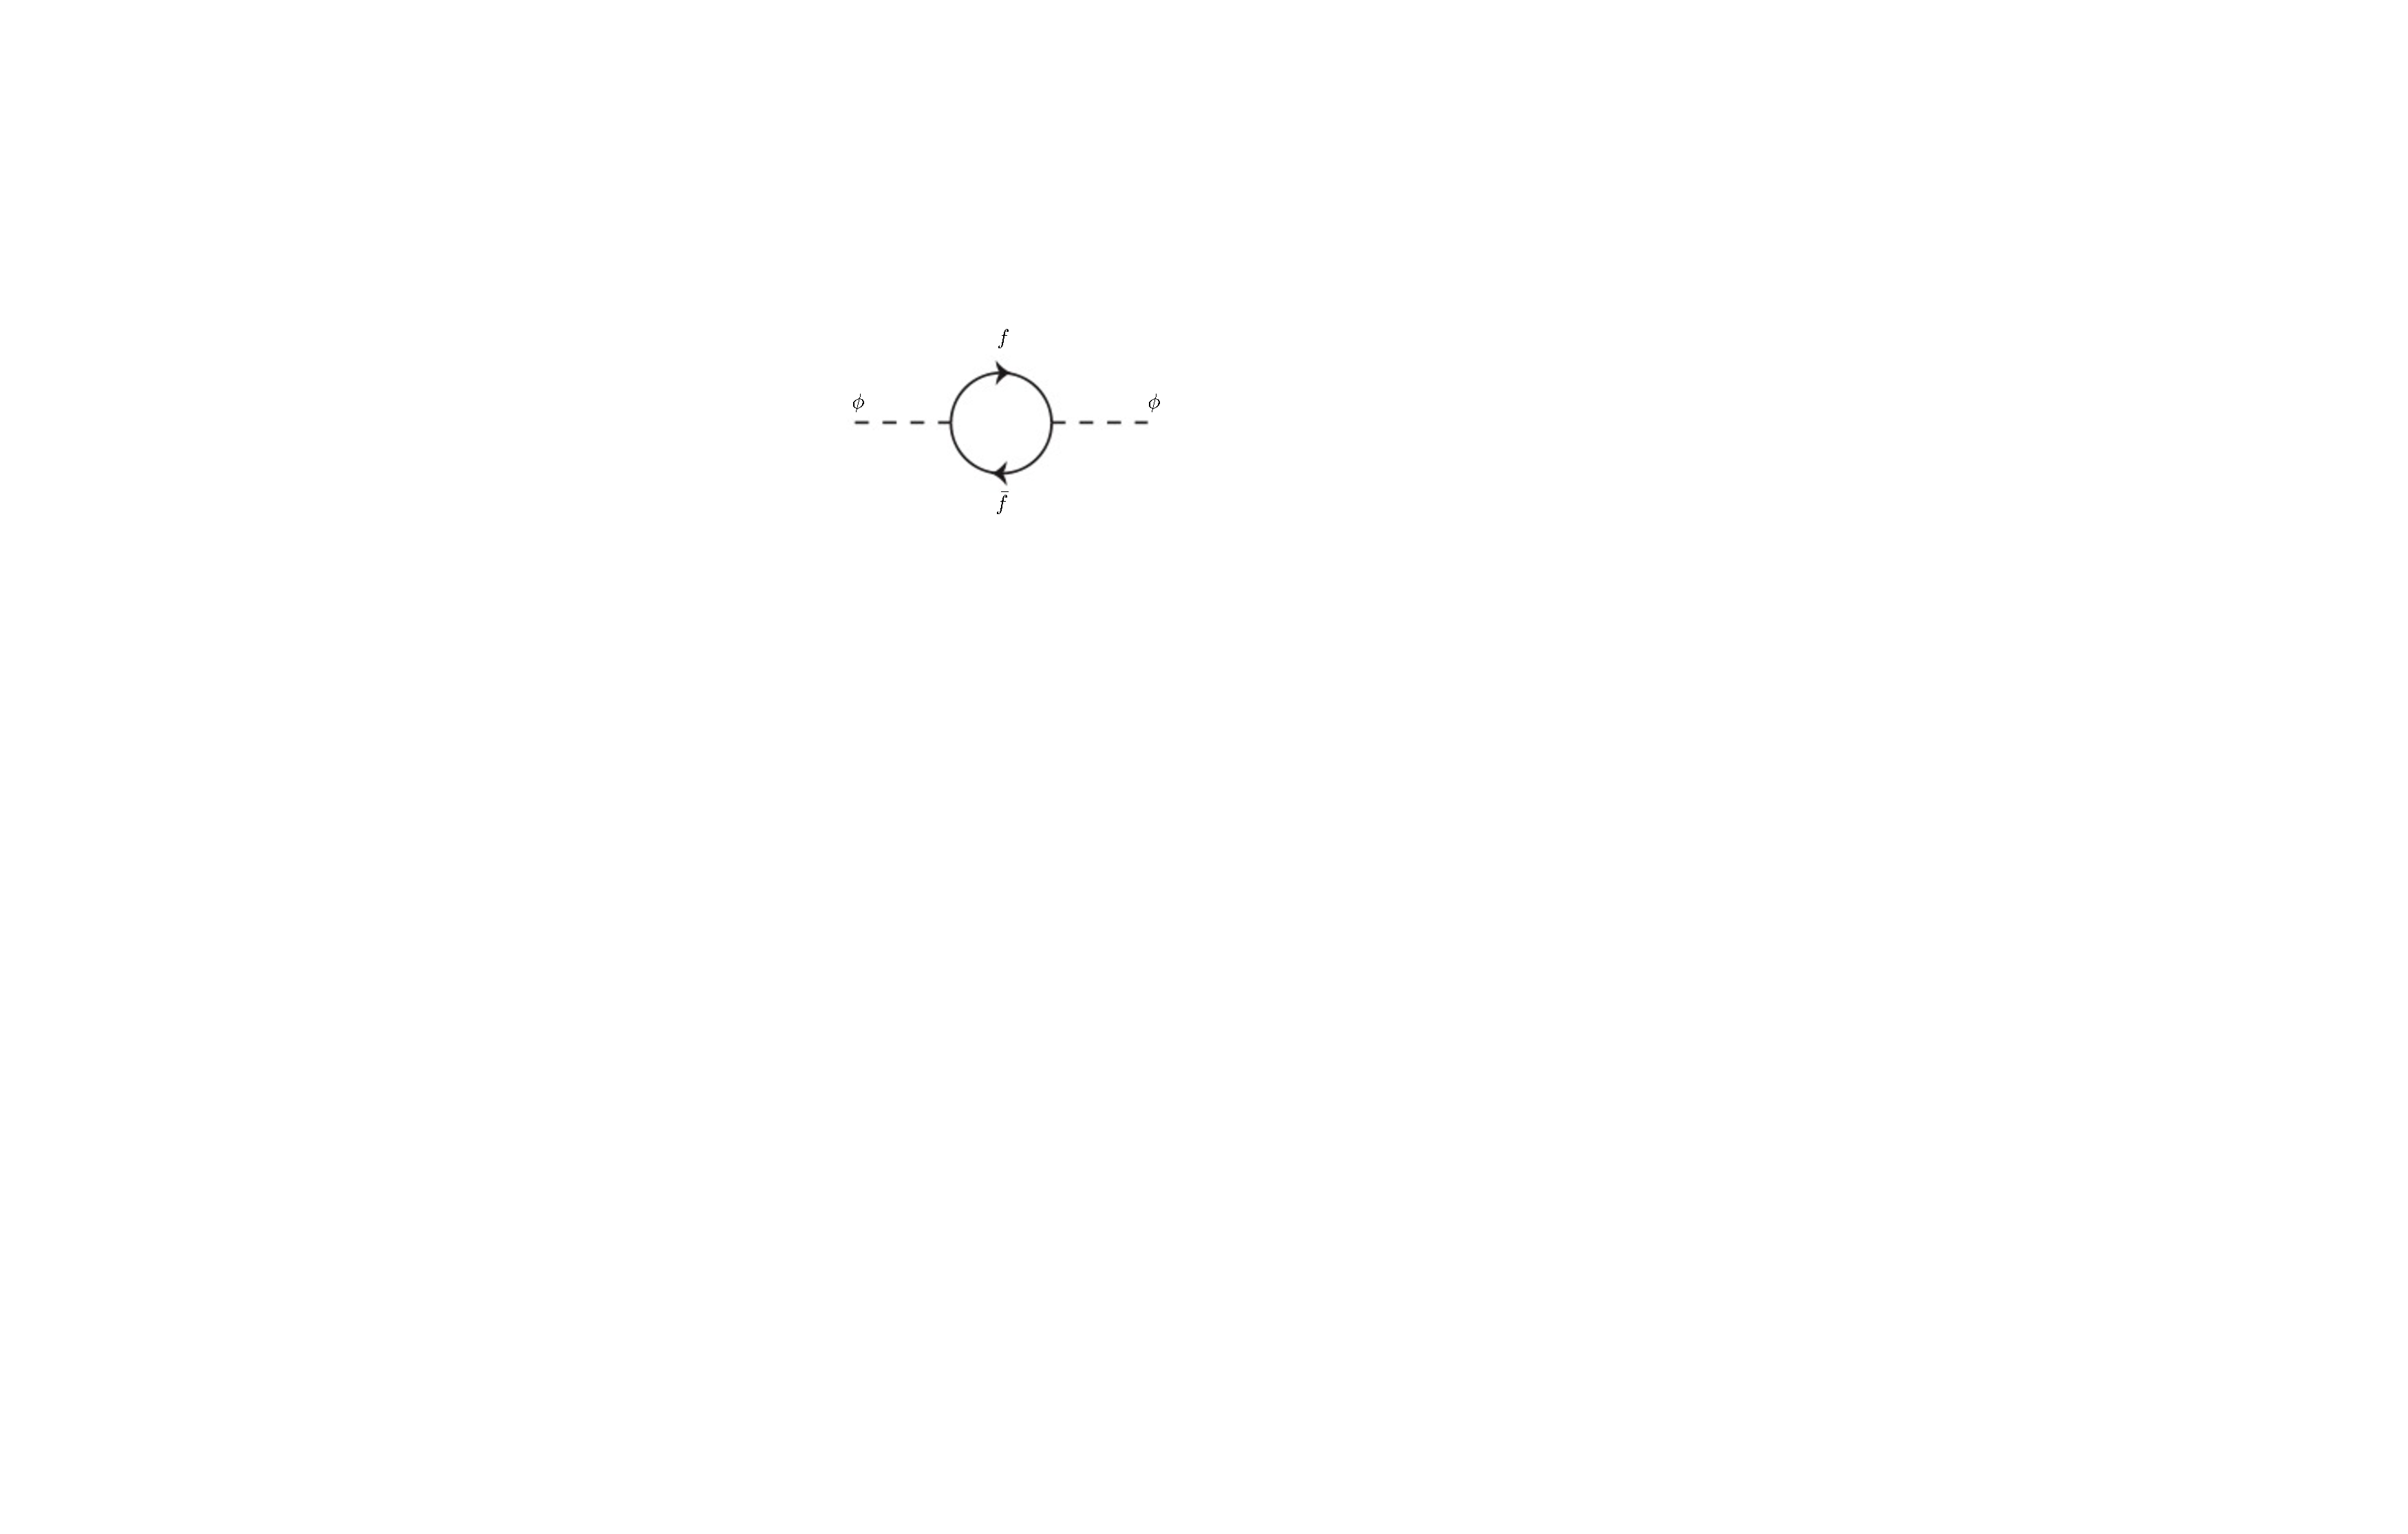
\includegraphics[width=0.45\textwidth]{plots/higgs_correction.pdf}
\caption[One loop quantum corrections to the Higgs squared massed parameter $m^{2}_{h}$ due to a fermion.]{One loop quantum corrections to the Higgs squared massed parameter $m^{2}_{h}$ due to a fermion.}  
\label{fig:higgscorrection}
\end{figure}

This can be demonstrated by considering the one loop quantum correction to the Higgs mass with a fermion f, shown in Figure \ref{fig:higgscorrection} with mass $m_{f}$. The Higgs field couples to f with a term in the Lagrangian $-\lambda_{f}h\bar{f}f$, yielding a correction of the form \cite{Martin:1997ns},
 
 \begin{equation}
 \delta m^{2}_{h} = -\frac{\lvert\lambda_{f}\rvert^{2}}{8\pi^{2}}\Lambda^{2} + �.. ,
 \end{equation}
 
 where $\lambda_{f}$ represents the coupling strength for each type of fermion $\propto m_{f}$, and $\Lambda$ the cutoff energy scale at which the \ac{SM} ceases to be a valid theory. 
 
 To recover the mass of the now discovered Higgs boson would require a fine-tuning of the parameters to cancel out these mass corrections the the Higgs mass to the scale of 30 orders of magnitude. This appears as an unnatural solution to physicists and it is this hierarchy problem that provides one of the strongest motivations for the theory of \acf{SUSY}.
 
\section{Supersymmmetry Overview}

\label{sec:susytheory}

Supersymmetry provides potential solutions to many of the issues raised in the previous section. It provides a dark matter candidate, can explain baryogenesis in the early universe and also provides an elegant solution to the hierarchy problem \cite{nilles1984supersymmetry}\cite{Haber:1984rc}\cite{Witten:1981nf}\cite{Wess197439}. At it's heart it represents a new space-time symmetry that relates fermions and bosons. This symmetry converts bosonic states into fermionic states, and vice versa, see Equation (\ref{susyoperator})  ,

\begin{equation}
\label{susyoperator}
Q \lvert Boson\rangle  = \lvert Fermion\rangle  \qquad Q \lvert Fermion\rangle = \lvert Boson\rangle,
\end{equation}
where the operator Q is the generator of these transformations. Quantum field theories which are invariant under such transformations are called supersymmetric.

This symmetry operator therefore acts upon a particles spin altering it by a half integer value. The consequences of the introduction of this additional space-time symmetry introduce a new rich phenomenology. For example in supersymmetric theories, both the left handed SU(2) doublet and right handed singlet of fermions will have a spin-0 superpartner, containing the same electric charge, weak isospin, and colour as its \ac{SM} partner. In the case of the leptons $(\nu_{l},l)_{L}$ will have two superpartners, a sneutrino $\widetilde{\nu_{l}}_{L}$ and a slepton $\widetilde{l}_{L}$, whilst the single $l_{R}$ also has a superpartner slepton $\widetilde{l}_{R}$. 
 
Each particle in a supersymmetric theory is paired together with their superpartners as a result of this supersymmetric transformations in a so called supermultiplet. These superpartners will then consequently also contribute to the corrections to the Higgs mass. Bosonic and fermionic loops contributing to the correction appear with opposite signs, and therefore cancellation of these divergent terms will stabilise the Higgs mass, solving the hierarchy problem \cite{muller2010introduction}\cite{aitchison2007supersymmetry}. 

One of the simplest forms of \ac{SUSY} would predict a whole set of supersymmetric partners to their \ac{SM} counterparts with the same mass and interactions. However the currently lack of any experimental evidence for the predicted sparticle spectrum implies \ac{SUSY} must be a broken symmetry in which any sparticle masses must be greater than their SM counterparts.

There exist many techniques which can induce supersymmetric breaking \cite{Intriligator:2007zz}\cite{Shadmi:2006jv}\cite{Burgess:2006mn}. Of particular interest to experimental physicists are those at which the breaking scale is of an order that is experimentally accessible to the \ac{lhc} i.e. $\sim$ \TeV scale. Whilst there is no requirement for supersymmetric breaking to occur at this energy scale, for supersymmetry to provide a solution to the hierarchy problem, it is necessary for this scale to not differ too drastically from the \ac{EWK} scale \cite{Murayama:2007sy}\cite{baer2006weak}.

 
\subsection{R-Parity}

\label{subsec:rparity}

Some supersymmetric theories also present a solution to the dark matter problem. Such theories can contain a \acf{LSP}, which matches the criteria of a \acf{WIMP} required by cosmological observation if R-parity is conserved.  

Baryon (B) and Lepton (L) number conservation is forbidden in the \ac{SM} by renormalisability requirements. The violation of Baryon or Lepton number would result in the proton lifetime much shorter than those set by experimental limits \cite{Martin:hep-ph9602349}. Another symmetry called R-parity is then often introduced to \ac{SUSY} theories to maintain baryon and lepton conservation. 

R-parity is described by the equation 

\begin{equation}
\label{eq:rparityequation}
R_{P} = (-1)^{3(B-L)+2s},
\end{equation}
where s represents the spin of the particles. $B =  \pm\frac{1}{3}$ for quarks/antiquarks and $B=0$ for all others, $L = \pm 1$ for leptons/antileptons, $L= 0$ for all others. 

R-parity ensures the stability of the proton in \ac{SUSY} models, and also has other consequences for the production and decay of supersymmetric particles. At particle colliders supersymmetric particles can only be pair produced, and similarly the decay of any produced supersymmetric particle is restricted to a \ac{SM} particle and a lighter supersymmetric particle as allowed by conservation laws. A further implication of R-parity is that once a supersymmetric particle has decayed to the \ac{LSP} it remains stable, unable to decay into a \ac{SM} particle.  

A \ac{LSP} would not interact in a detector at a particle collider, leaving behind a missing energy $\met$ signature. The assumption of R-parity and its consequences are used to determine the physical motivation and search strategies for \ac{SUSY} model at the \ac{lhc}. 

\section{Experimental signatures of SUSY at the LHC}
\label{sec:susysearches}

Should strongly interacting sparticles be within the experimental reach of the \ac{lhc}, then it is expected that they can be produced in a variety of ways. 

\begin{itemize}
\item squark/anti-squark and gluino pairs can be produced via both gluon fusion and quark/anti-quark scattering.
\item a gluino and squark produced together via quark-gluon scattering
\item squark pairs produced via quark-quark scattering
\end{itemize}

Whilst most \ac{SUSY} searches invoke the requirement of R-parity to explore parameter phase space, there still exist a whole plethora of possible \ac{SUSY} model topologies which could be discovered at the \ac{lhc}. 

During the 2011 run period at a $\com = 7$ \TeV particular models were used to benchmark performance and experimental reach of both \ac{CMS} searches and previous experiments. The \acf{CMSSM} was initially chosen for a number of reasons \cite{Kane:1993td}. One of the most compelling being the reduction from the up to 105 new parameters introduced by \ac{SUSY} in addition to the existing 19 of the \ac{SM} to that of just 5 free extra free parameters. It was this simplicity, combined with the theory not requiring any fine tuning of particle masses to produce the experimentally verified \ac{SM} that made it an attractive model to interpret physics results. 

However recent results from the \ac{lhc} now strongly disfavour large swathes of \ac{CMSSM} parameter space \cite{Strege:2011pk}\cite{Citron:2012fg}\cite{Ghosh:2012dh}. In the face of such results a more pragmatic model independent search strategy is now applied across most \ac{SUSY} searches at the \ac{lhc}, see Section (\ref{subsec:sms}). 

As previously stated, a stable \ac{LSP} that exhibits the properties of a dark matter would be weakly interacting and therefore will not be directly detected in a detector environment. Additionally the cascade decays of supersymmetric particles to the \ac{LSP} would also result in significant hadronic activity. These signatures can then be characterised through large amounts of hadronic jets (see Section (\ref{subsec:cmsobjects-jets})), leptons and a significant amount of missing energy dependent upon the size of the mass splitting between the \ac{LSP} and the supersymmetric particle it has decayed from.

Whilst the \ac{SM} contains processes which can exhibit a similar event topology to that described above. The largest contribution of which comes in from the general QCD environment of a hadron collider. A multitude of different analytical techniques are used by experimental physicists to reduce or estimate any reducible or irreducible backgrounds, allowing a possible \ac{SUSY} signature to be extracted. The techniques employed within this thesis are described in great detail within Section (\ref{sec:alphatintroduction}).

\subsection{Simplified Models}

\label{subsec:sms}

With such a variety of different ways for a \ac{SUSY} signal to manifest itself, it is necessary to be able to interpret experimental reach through the masses of gluinos and squarks which can excluded by experimental searches rather than on a model specific basis. This is accomplished through \ac{SMS} models, which are specific \ac{SUSY} decays which contain only one process. For example Figure \ref{fig:susydecayexamples} shows two particular decays; the production of a pair of gluinos (the superpartner to the gluon) or squarks which then decay into \ac{SM} particles and the \ac{LSP}.

\begin{figure}[ht]
\centering
\begin{minipage}[b]{0.45 \linewidth}
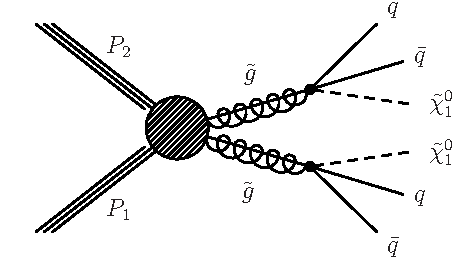
\includegraphics[width = 1.0\linewidth]{plots/t1susydecay.pdf}
\end{minipage}
\quad
\begin{minipage}[b]{0.45\linewidth}
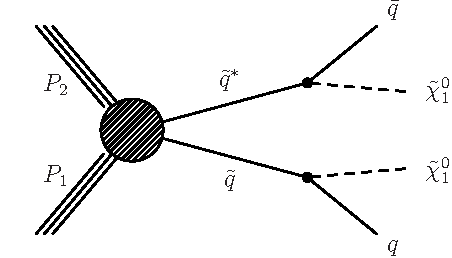
\includegraphics[width = 1.0\linewidth]{plots/t2susydecay.pdf}
\end{minipage}
\caption[Two example \ac{SMS} model decays (T1 (left),T2 (right) \cite{Chatrchyan:2013sza}), which are used in interpretations of physics reach by \ac{CMS}.]{Two example \ac{SMS} model decays (T1 (left),T2 (right) \cite{Chatrchyan:2013sza}), which are used in interpretations of physics reach by \ac{CMS}. }
\label{fig:susydecayexamples}
\end{figure}

In both of these scenarios a set decay topology with a 100$\%$ branching ratio is assumed.

Searching and interpreting \ac{SUSY} searches in this way�.

The convention for the naming of these \ac{SMS} models is via the prefix...

  \chapter{The LHC and the CMS Detector}
\label{chap:cmsoverview}

Probing the \ac{SM} for signs of new physics would not be possible without the immensely complex electronics and machinery that has made the TeV energy scale accessible to physicists for the first time. This chapter will introduce both the \ac{lhc} based at \acf{CERN}  and the \acf{CMS} detector (of which the author is a member). Section (\ref{sec:cmsdetector}) serves to present an overview of the different components of  the \ac{CMS} detector, with specific components relevant to the search for supersymmetric particles described in greater detail. Section (\ref{sec:cmsobjects}) will focus on event and object reconstruction, again, with more emphasis on jet level quantities which are most relevant to the author's analysis research. Finally, Section (\ref{sec:triggersystem}) will describe and detail the service work for the \ac{CMS} Collaboration performed by the author, in measuring the performance of L1 single jet triggers in the \acf{GCT} during the 2012-2013 run period.  

\section{The LHC}
\label{sec:thelhc} 

The \ac{lhc} is a storage ring, accelerator, and collider of circulating beams of protons or ions. Housed in the tunnel dug for \acf{LEP}, it is approximately 27km in circumference, 100m underground, and straddles the border between France and Switzerland, outside of Geneva. It is currently the only collider in operation that is able to study physics at the TeV scale.  A double-ring circular synchrotron, it was
designed to collide both proton-proton (pp) and heavy ion (PbPb) with a centre of mass energy $\sqrt{s} = $ 14 \TeV at a final design luminosity of $10^{34}$cm$^{-2}$s$^{-1}$. \\

These counter-circulating beams of protons or Pb ions are merged in four sections around the ring to enable collisions of the beams, with each interaction point being home to one of the four major experiments; \acf{ALICE} \cite{alicetdr}, \acf{ATLAS} \cite{atlastdr}, \acf{CMS} \cite{cmstdr} and \acf{LHCb} \cite{lhcbtdr} which record the resultant collisions. The layout of the \ac{lhc} ring is shown in Figure \ref{fig:lhc-ring}. The remaining four sections contain acceleration, collimation and beam dump systems. In the eight arc sections, the beams are steered by magnetic fields of up to 8 \T provided by super conduction dipole magnets, which are maintained at temperatures of 2 \K using superfluid helium. Additional magnets for focusing and corrections are also present in straight sections within the arcs and near the interaction regions where the detectors are situated. \\


\begin{figure}[!h]

\centering
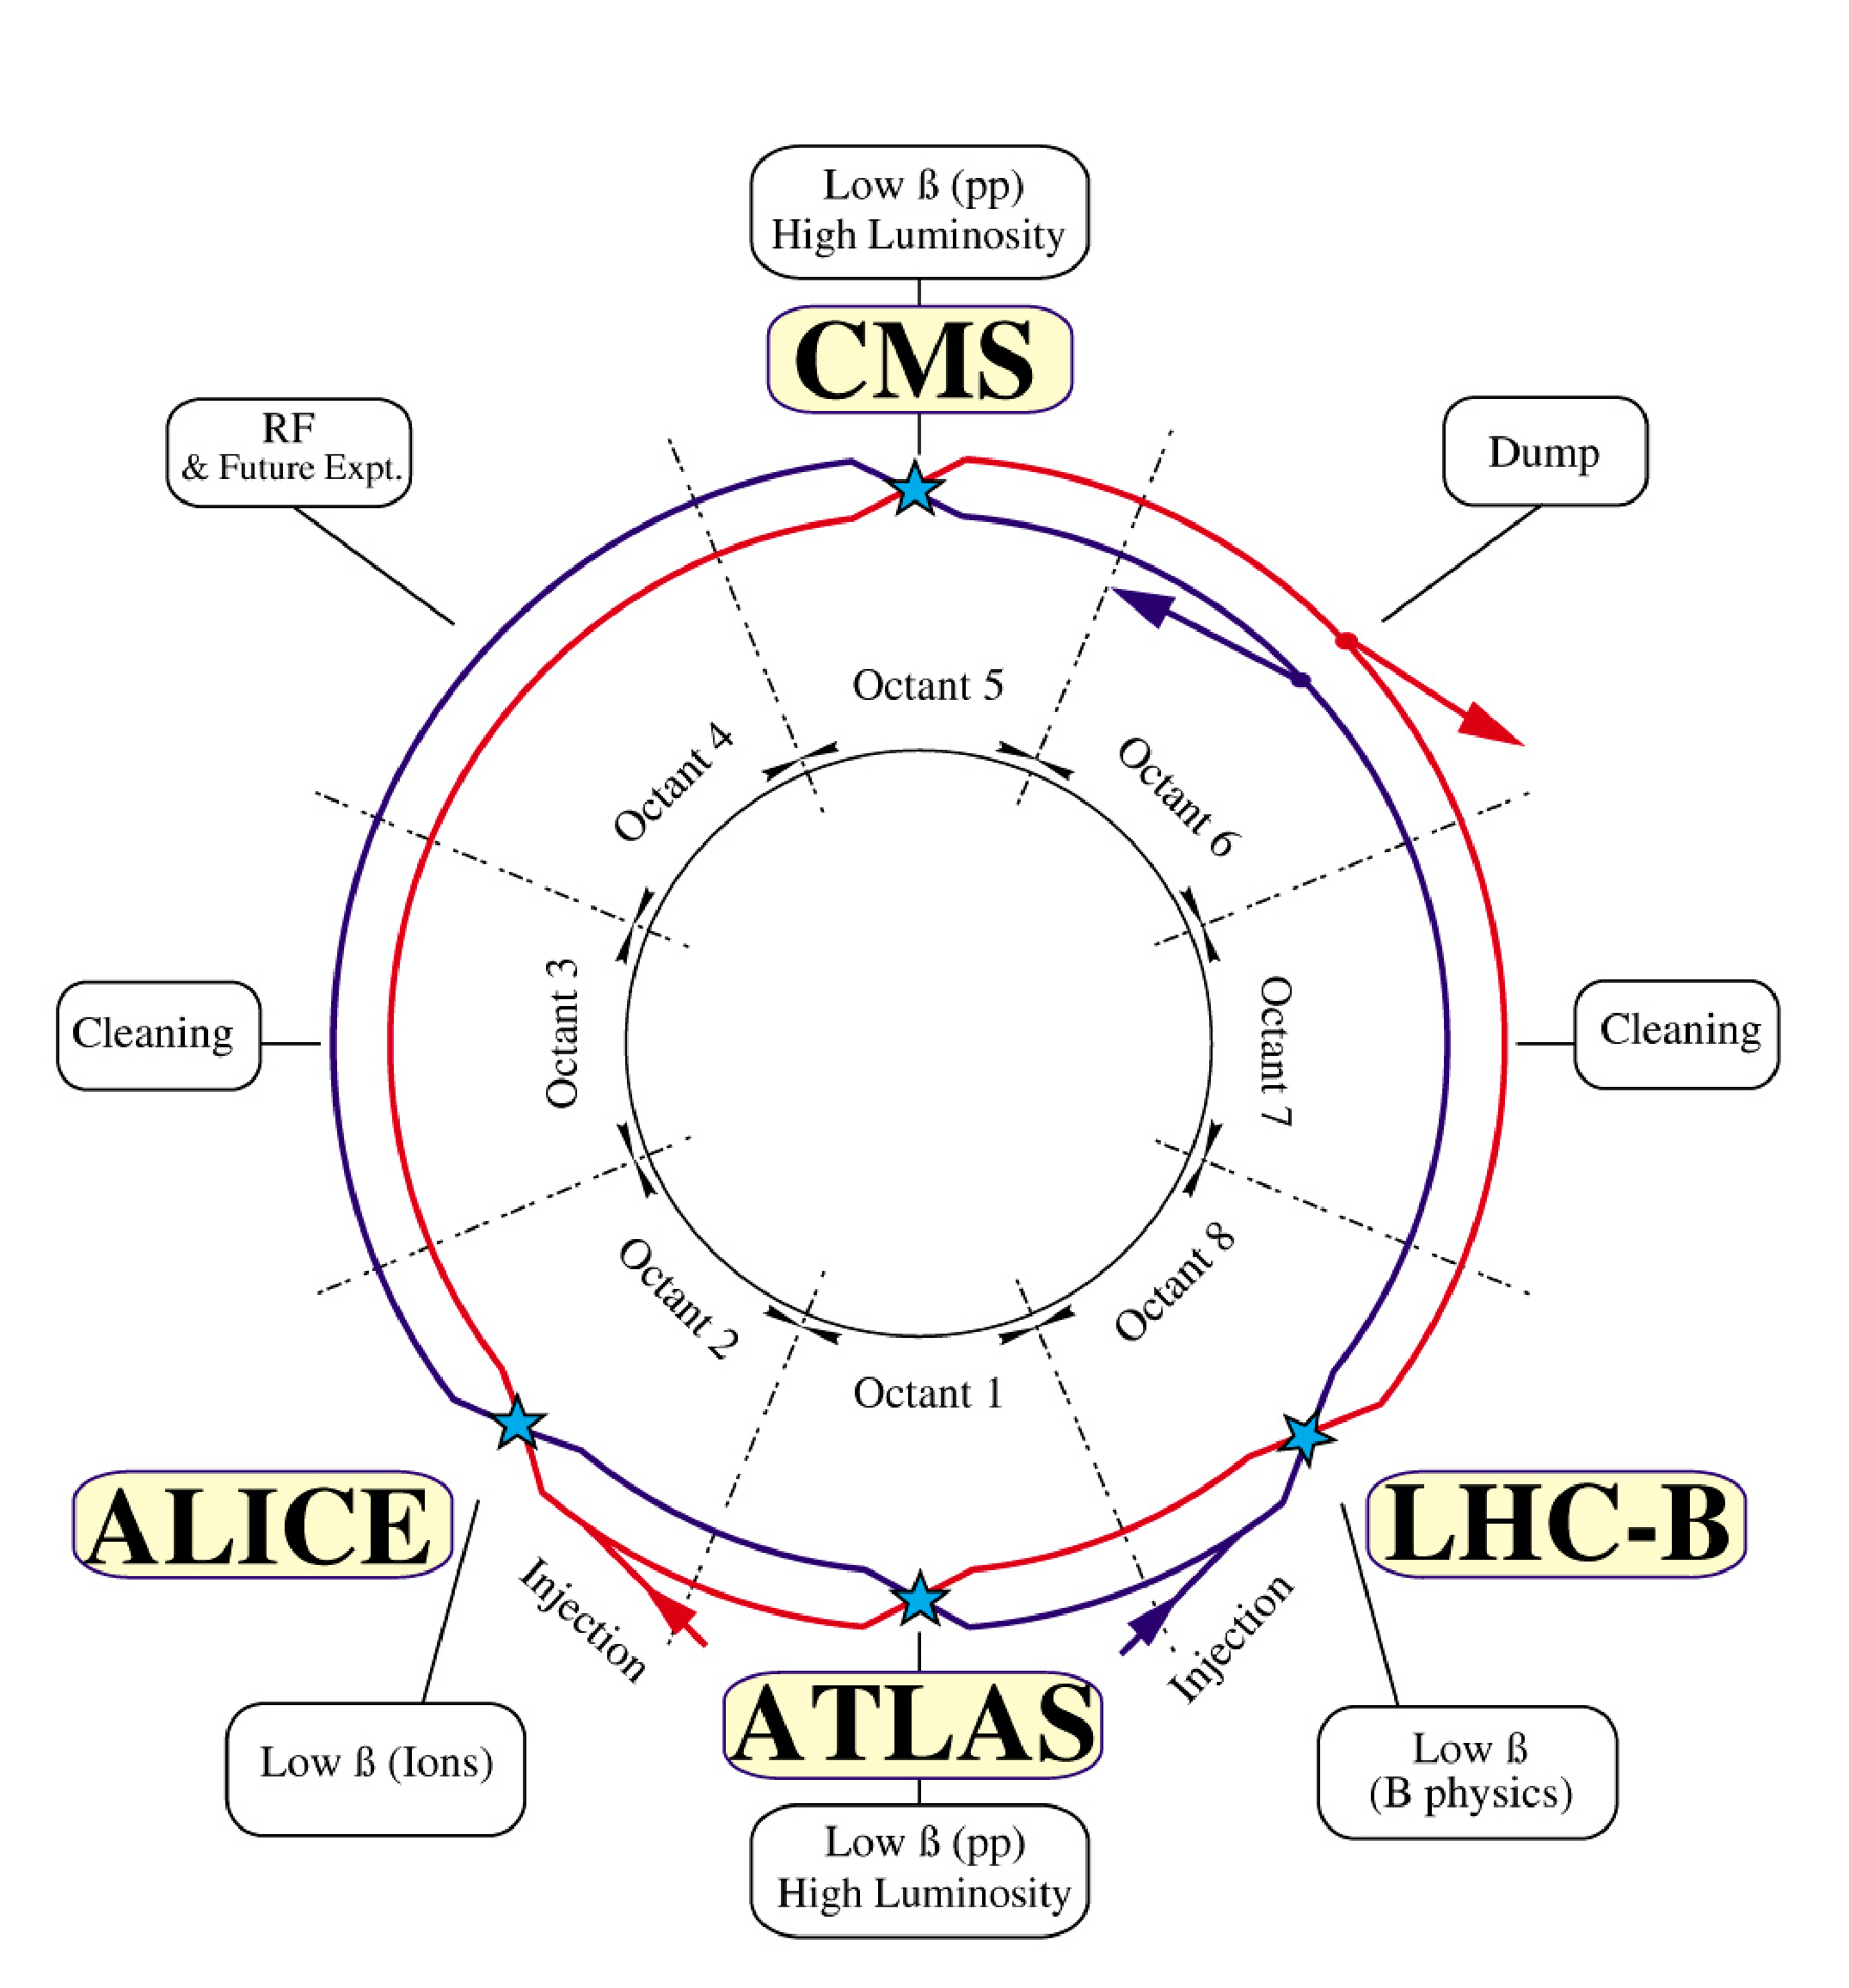
\includegraphics[width=0.60\textwidth]{plots/lhc-ring-photo.pdf}
\caption[A top-down layout of the \LHC, with the position of the four main detectors labelled.]{A top down layout of the \LHC. \cite{Jean-Luc:841573}, with the position of the four main detectors labelled.}  
\label{fig:lhc-ring}
\end{figure}


Proton beams are formed inside the \acf{PS} from bunches of protons 50 \ns apart with an energy of 26 \GeV. The protons are then accelerated in the \acf{SPS} to 450 \GeV  before being injected into the \ac{lhc}. These \ac{lhc} proton beams consists of many ``bunches" (i.e. approximately $1.1 \times 10^{11}$  protons localised into less than 1 \ns in the direction of motion).  Before collision, the beams are ramped to 4 \TeV (2012) per beam, in a process involving increasing the current passing through the dipole magnets. Once the desired \com energy is reached then the beams are allowed to collide at the interaction points. The luminosity falls regularly as the run progresses; protons are lost in collisions, and eventually the beam is dumped before repeating the process again. 

Colliding the beams produced an instantaneous luminosity of approximately 5 $\times$ 10$^{33}$ cm$^{-2}$s$^{-1}$ during the 2012 run. The high number of protons in each bunch increases the likelihood of multiple interactions with each crossing of the counter-circulating beams. This leads to isotropic energy depositions within the detectors positioned at these interaction points, increasing the energy scale of the underlying event. This is known as pile-up and the counteracting of its effects are important to the many measurements performed at the \ac{lhc}.

In the early phase of prolonged operation, after the initial shutdown, the machine operated in 2010-2011 at 3.5 \TeV per beam, \com $=$ 7 \TeV, delivering 6.13 \fb of data \cite{LHClumo}. During the 2012-2013 run period, data was collected at an increased \com $=$ 8 \TeV improving the sensitivity of searches for new physics. Over the whole run period 23.3 \fb of data was delivered, of which 21.8 \fb was recorded by the \ac{CMS} detector as shown in Figure \ref{fig:lhc-lumo} \cite{LHClumo}. A total of 12 \fb of 8 \TeV certified data was collected by October 2012, and it is this data which forms the basis of the results presented within this thesis.

\begin{figure}[!h]
\centering
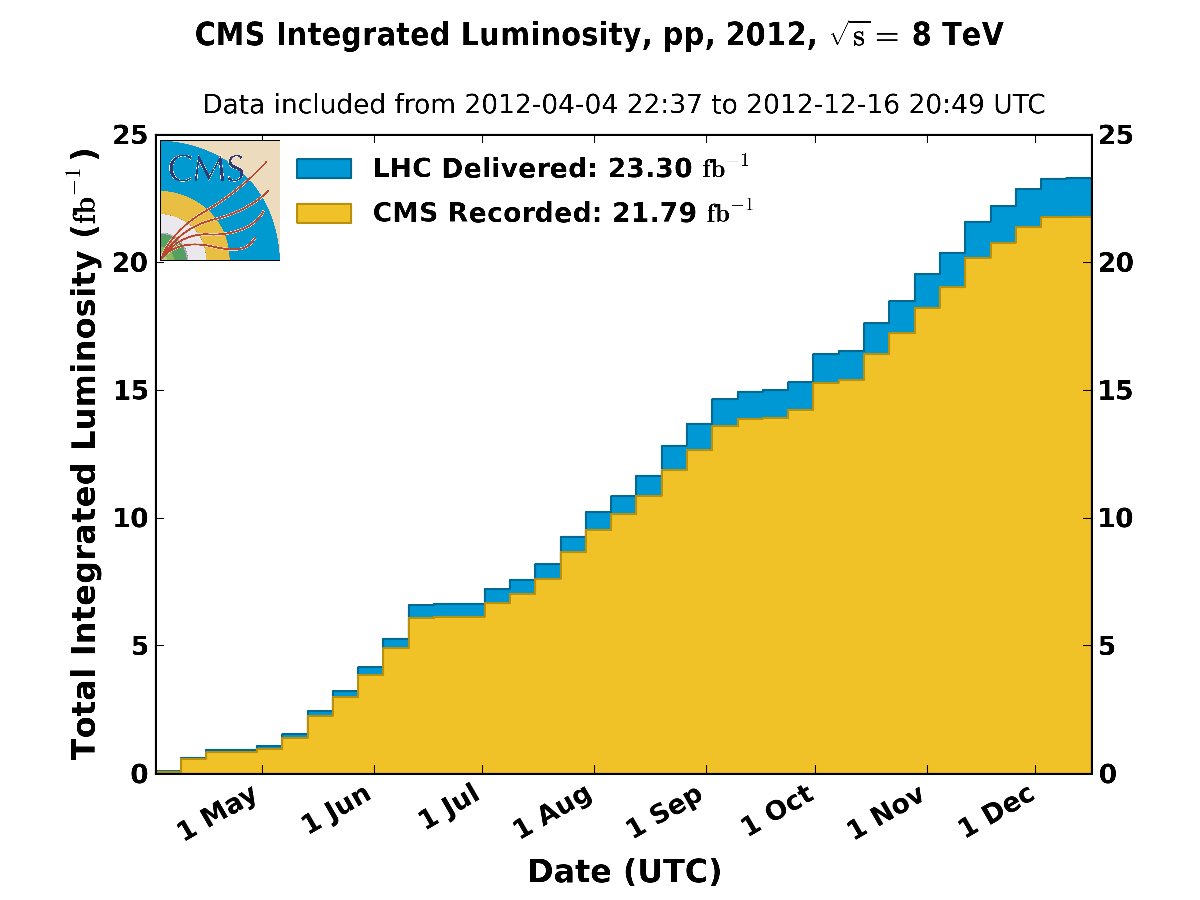
\includegraphics[width=0.60\textwidth]{plots/lhc-lumo-8tev.pdf}
\caption[The total integrated luminosity delivered to and collected by \ac{CMS} during the 2012 8 \TeV \pp runs]{The total integrated luminosity delivered to and collected by \ac{CMS} during the 2012 8 \TeV \pp runs.}  
\label{fig:lhc-lumo}
\end{figure}


\section{The CMS Detector}
\label{sec:cmsdetector}

The \acf{CMS} detector is one of two general purpose detectors at the \ac{lhc} designed to search for new physics. The detector is designed to provide efficient identification and measurement of many physics objects including photons, electrons, muons, taus, and hadronic showers over wide ranges of transverse momentum and direction. Its nearly 4$\pi$ coverage in solid angle allows for accurate measurement of global transverse momentum imbalance. These design factors give \ac{CMS} the ability to search for direct production of \ac{SUSY} particles at the \TeV scale, making the search for Supersymmetric particles one of the highest priorities among the wide range of physics programmes at \ac{CMS}. 

\ac{CMS} uses a right-handed Cartesian coordinate system with the origin at the interaction point and the z-axis pointing along the beam axis. The x-axis points radially inwards to the centre of the collider ring, with the y-axis points vertically upward. The azimuthal angle $\phi$, ranging between [$-\pi$,$\pi$], is defined in the x-y plane starting from the x-axis. The polar angle $\theta$ is measured from the z axis. The common convention in particle physics is to express an out-going particle in terms of $\phi$ and its pseudorapidity defined as

\begin{equation}
\eta = -\log\tan\left(\frac{\theta}{2}\right).
\end{equation}

The variable $\Delta R = \sqrt{\Delta\phi^{2} + \Delta\eta^{2} } $ is commonly used to define angular distance between objects within the detector. Additionally, energy and momentum is typically measured in the transverse plane perpendicular to the beam line. These values are calculated from the x and y components of the object and are denoted as $\et = E\sin\theta$ and $\pt = \sqrt{p^{2}_{x}+p^{2}_{y}}$. 

\subsection{Detector Subsystems}
\label{subsec:detectorsubsystems}

As the range of particles produced from \pp collisions interact in different ways with matter, \ac{CMS} is divided into sub-detector systems, which perform complementary roles to identify the identity, mass, and momentum of the different physics objects present in each event. These detector sub-systems contained within \ac{CMS} are wrapped in layers around a central 13m long 4 \T super conducting solenoid, as shown in Figure \ref{fig:cms-detector}. With the endcaps closed, \ac{CMS} is a cylinder of length 22m, diameter 15m, and mass 12.5 kilotons. A more detailed complete description of the detector can be found elsewhere \cite{cmstdr}. \\

\begin{figure}[!h]

\centering
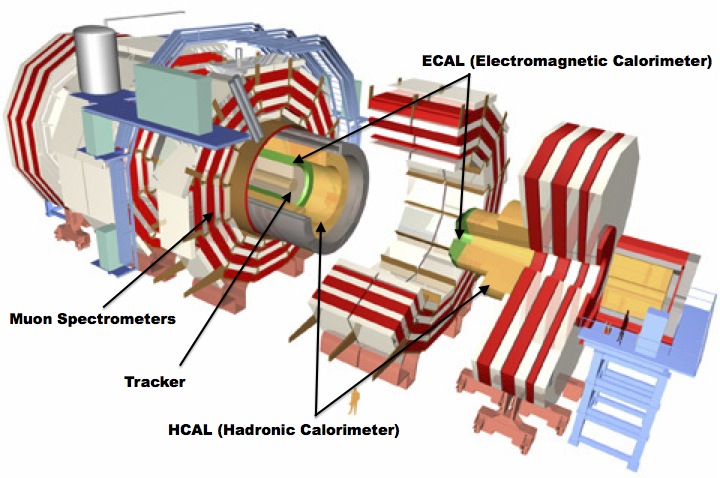
\includegraphics[width=0.65\textwidth]{plots/cms-detector.pdf}
\caption[A pictorial depiction of the \ac{CMS} detector.]{A pictorial depiction of the \ac{CMS} detector with the main detector subsystems labelled.   \cite{cms-public-detector}}  
\label{fig:cms-detector}
\end{figure}

\subsection{Tracker}
\label{subsec:tracker}

 The inner-most sub-detector of the barrel is the multi-layer silicon tracker, formed of a pixel detector component encased by layers of silicon strip detectors. The pixel detector consists of three layers of silicon pixel sensors providing measurements of the momentum, position coordinates of the charged particles as they pass, and the location of primary and secondary vertices between 4 cm and 10 cm transverse to the beam. Outside the pixel detector, ten cylindrical layers of silicon strip detectors extend the tracking system out to a radius of 1.20 m from the beam line. The tracking system provides efficient and precise determination of the charges, momenta, and impact parameters of charged particles, with the geometry of the tracker extending to cover a rapidity range up to $\lvert\eta\rvert \textless$ 2.5.  \\
 
 The tracking system also plays a crucial part in the identification of jets that originate from b-quarks through the measurement of displaced secondary vertices. The methods in which these b-flavoured jets are identified are discussed within Section (\ref{subsec:cmsobjects-btagging}). The identification of b-jets is important in many searches for natural \ac{SUSY} models and forms an important part of the inclusive search strategy described within Section (\ref{subsec:searchstrategy}).
 
\subsection{Electromagnetic Calorimeter}
\label{subsec:ecal}

 Immediately outside of the tracker, but still within the magnet core, sits the \acf{ECAL}. Covering a pseudorapidity up to $\lvert\eta\rvert < 3$ and comprising of over 75 $\times 10^{3}$ PbWO$_{4}$ (lead tungstate) crystals that scintillate as particles deposit energy, the \ac{ECAL} provides high resolution measurements of the electromagnetic showers from photons and electrons in the detector. \\ 
 
 Lead tungstate is used because of its short radiation length ($X_{0} \sim 0.9$ cm) and small Molier\'{e} radius ($\sim 2.1$ cm) leading to high granularity and resolution. Its fast scintillation time ($\sim 25$ ns) reduces the effects of pile-up, which occurs when energy from previous collisions are still being read out, and its radiation hardness gives it longevity. The crystals are arranged in modules which surround the beam line in a non-projective geometry,  angled at 3$^{\circ}$, with respect to the interaction point to minimise the risk of particles escaping down the cracks between the crystals.\\
 
 The  \ac{ECAL} is primarily composed of two sections, the \acf{EB} which extends in pseudo-rapidity to $\lvert\eta\rvert < 1.479$ with a crystal front cross section of 22$\times$22 mm and a length of 230 mm corresponding to 25.8 radiation lengths. The \acf{EE} covers a rapidity range of $1.479 < \lvert\eta\rvert < 3.0 $, which consists of two identical detectors
on either side of the \ac{EB}.  A lead-silicon sampling `pre-shower' detector \acf{ES} is placed before the endcaps to aid in the identification of neutral pions. Their arrangement is shown in Figure \ref{fig:cms-ecal}. \\

 
 \begin{figure}[!h]

\centering
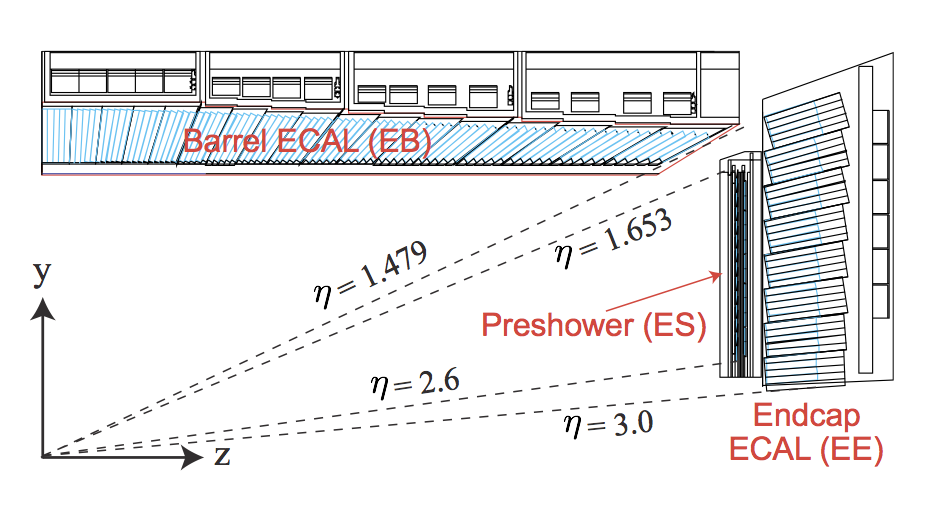
\includegraphics[width=0.85\textwidth]{plots/cms-ecal.pdf}
\caption[Illustration of the \ac{CMS} \ac{ECAL}. ]{Illustration of the \ac{CMS} \ac{ECAL} showing the arrangement of the lead tungstate crystals in the \ac{EB} and \ac{EE}. The \ac{ES} is also shown and is located in front of the \ac{EE} \cite{CMS_ECAL_TDR}.}  
\label{fig:cms-ecal}
\end{figure}


Scintillation photons from the lead tungstate crystals are instrumented with \acf{APD} and \acf{VPT}, located in the \ac{EB} and \ac{EE} respectively. They convert the scintillating light into an electric signal which is consequently used to determine the amount of energy deposited within the crystal. These instruments are chosen for their resistance under operation to the strong magnetic field of \ac{CMS}. The scintillation of the \ac{ECAL} crystals, as well as the response of the \ac{APD}s, varies as a function of temperature; and so cooling systems continually maintain an overall constant \ac{ECAL} temperature $\pm 0.05 ^{\circ}C$.
 

\subsection{Hadronic Calorimeter}
\label{subsec:hcal} 

Beyond the \ac{ECAL} lies the \acf{HCAL} which is responsible for the accurate measurement of hadronic showers, crucial for analyses involving jets or missing energy signatures. The \ac{HCAL} is a sampling calorimeter which consists of alternating layers of brass absorber and plastic scintillator. The exception being in the hadron forward ($3.0 < \lvert\eta\rvert < 5.0 $) region in where steel absorbers and quartz fibre scintillators are used because of their increased radiation tolerance. Hadron showers are initiated in the absorber layers inducing scintillation in the plastic scintillator tiles.  These scintillation photons are converted by wavelength shifting fibres for read-out by hybrid photodiodes. \\

The \ac{HCAL}'s size is constrained to a compact size by the presence of the solenoid, requiring the placement of an additional outer calorimeter on the outside of the solenoid to increase the sampling depth of the \ac{HCAL}. A schematic of the \ac{HCAL} can be seen in Figure \ref{fig:cms-hcal}.\\
 
 \begin{figure}[!h]

\centering
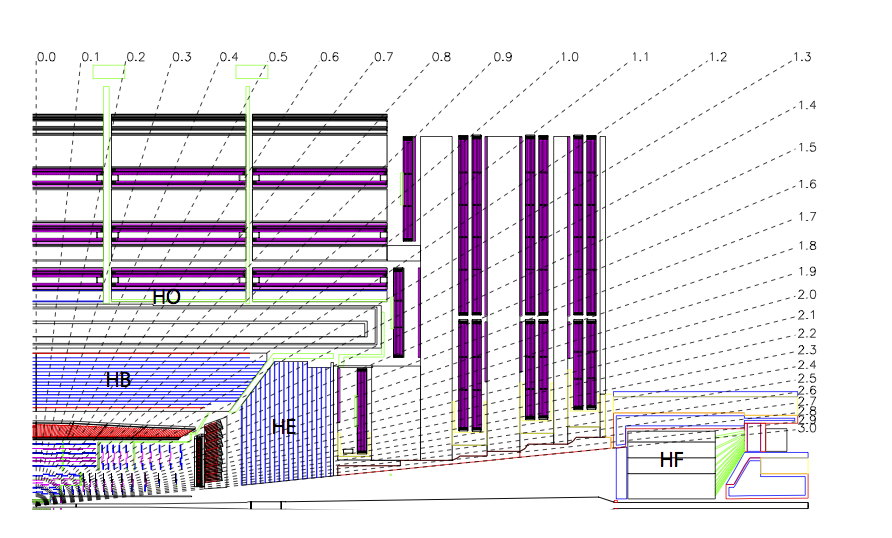
\includegraphics[width=0.85\textwidth]{plots/cms-hcal.pdf}
\caption[Schematic of the \ac{CMS} \acf{HCAL}.]{ Schematic of the hadron calorimeters in the r-z plane, showing the locations of the \ac{HCAL} components and the \ac{HF}. \cite{cmstdr}.}  
\label{fig:cms-hcal}
\end{figure}
 
The \ac{HCAL} covers the range $\lvert\eta\rvert < 5$ and consists of four sub-detectors: the \ac{HB}  $\lvert\eta\rvert < 1.3$, the \acf{HO}, the \acf{HE} $1.3 < \lvert\eta\rvert < 3.0 $ and the \acf{HF}.  The \ac{HB}, contained between the outer edge of the \ac{ECAL} and the inner edge of the solenoid is formed of 36 azimuthal wedges which are split between two half-barrel segments. Each wedge is segmented into four azimuthal angle ($\phi$) sectors, and each half-barrel is further segmented into 16 $\eta$ towers. The electronic readout chain, channels the light from the active scintillator layers from one $\phi$-segment and all $\eta$-towers of a half-barrel to a \acf{HPD}.

The relatively short number of interaction lengths ($\lambda_{l}$, the distance a hadron will travel through the absorber material before it has lost $\frac{1}{e}$ of its energy) within the \ac{HB}, the lowest being $\lambda_{l}$ = 5.82 at $\lvert\eta\rvert = 0$, facilitates the need for the `tail catching' \ac{HO} to increase the sampling depth in the central barrel rapidity region $\lvert\eta\rvert < 1.3$ to 11 interaction lengths. Significant fractions of the hadrons energy will be deposited in the \ac{ECAL} as it passes through the detector. Therefore, measurements of hadron energies in the central regions $\lvert\eta\rvert < 3.0$ use both the \ac{ECAL} and \ac{HCAL} to reconstruct the true energy from showering hadrons. 

\subsection{Muon Systems}
\label{subsec:muonsystems} 
 
Muons being too massive to radiate away energy via Bremsstrahlung, interact little in the calorimeters and mostly pass through the detector until they reach the system of muon detectors which forms the outer most part of the \ac{CMS} detector.  

Outside of the superconducting solenoid are four muon detection layers interleaved with the iron return yokes, which measure the muons energy via ionisation of gas within detector elements. Three types of gaseous chambers are used. The \acf{DT}, \acf{CSC}, and \acf{RPC} systems provide efficient detection of muons with pseudo-rapidity $\lvert\eta\rvert < 2.4 $. The best reconstruction performance is obtained when the muon chamber is combined with the inner tracking information to determine muon trajectories and their momenta \cite{CMS_MUON_TDR}.  \\ 

\section{Event Reconstruction and Object Definition}
\label{sec:cmsobjects}

The goal of event reconstruction is to take the raw information recorded by the detector and to compute from it higher-level quantities which can be used at an analysis level. These typically correspond to an individual particle's energy and momenta, or groups of particles which shower in a narrow cone, the overall global energy and momentum balance of the event. The reconstruction of these objects are described in great detail in \cite{CMS_TDR_PHYS_vol1}, while covered below are brief descriptions of those which are most relevant to the analysis detailed in Chapter \ref{chap:SUSYsearches}.

\subsection{Jets}
\label{subsec:cmsobjects-jets}

Quarks and gluons are produced copiously at the LHC in the hard scattering of partons. As these quarks and gluons fragment, they hadronize and decay into a group of strongly interactive particles and their decay products. These streams of particles travel in the same direction, as they have been ``boosted" by the momentum of the primary hadron. These collections of decay products are reconstructed and identified together as a ``jet''.

At \ac{CMS} jets are reconstructed from energy deposits in the detector via the anti-kt algorithm \cite{antiktalgo} with size parameter $\Delta R = 0.5$. The anti-kt jet algorithm clusters jets by defining a distance between hard (high $\pt$) and soft (low $\pt$) particles such that soft particles are preferentially clustered with hard particles before being clustered between themselves. This produces jets which are robust to soft particle radiation from the pile-up conditions produced by the \ac{lhc}. 

There are two main types of jet reconstruction used at \ac{CMS}, Calorimeter (\Calo) and Particle Flow (\PF) jets \cite{CMS-PAS-JME-10-003}. Calorimeter jets are reconstructed using both the \ac{ECAL} and \ac{HCAL} cells, combined into calorimeter towers. These calorimeter towers consist of geometrically matched \ac{HCAL} cells and \ac{ECAL} crystals. Electronics noise is suppressed by applying a threshold to the calorimeter cells, with pile-up effects reduced by a requirement placed on the tower energy  \cite{Janssen:1322145}. Calorimeter jets are the jets used within the analysis presented in this thesis.  

\PF jets are formed from combining information from all of the \ac{CMS} sub-detectors systems to  determine which final state particles are present in the event. Generally, any particle is expected to produce some combination of a track in the silicon tracker, a deposit in the calorimeters, or a track in the muon system. The \PF jet momentum and spatial resolutions are greatly improved with respect to calorimeter jets, as the use of the tracking detectors and of the high granularity of \ac{ECAL} allows resolution and measurement of charged hadrons and photons inside a jet,  which together constitute $\sim$ 85$\%$ of the jet energy \cite{1748-0221-6-11-P11002}.

The jets reconstructed by the clustering algorithm in \ac{CMS} typically have an energy that differs to the `true' energy measured by a perfect detector. This stems from the non-linear and nonuniform response of the calorimeters as well as other residual effects including pile-up and underlying events. Therefore, additional corrections are applied to recover a uniform relative response as a function of pseudo-rapidity. These are applied as separate sub corrections \cite{1742-6596-404-1-012014}. 

\begin{itemize}

\item A pile-up correction is first applied to the jet. It subtracts the average extra energy deposited in the jet that comes from other vertices present in the event and is therefore not part of the hard jet itself.
\item $\pt$ and $\eta$ dependant corrections derived from Monte Carlo simulations are used to account for the non-uniform response of the detector.\item $\pt$ and $\eta$ residual corrections are applied to data only to correct for difference between data and Monte Carlo. The residual is derived from QCD di-jet samples and the $\pt$ residual from $\gamma + $ jet and $Z + $ jets samples in data.

\end{itemize}

\subsection{B-tagging}
\label{subsec:cmsobjects-btagging}

The decays of b quarks are suppressed by small \CKM matrix elements. As a result, the lifetimes of b-flavoured hadrons, produced in the fragmentation of b quarks, are relatively long; $\mathcal{O}$ 1ps. The identification of jets originating from b quarks is very important for searches for new physics and for measurements of \ac{SM} processes.  \\

Many different algorithms developed by \ac{CMS} select b-quark jets based on variables such as; the impact parameters of the charged-particle tracks, the properties of reconstructed decay vertices, and the presence or absence of a lepton, or combinations thereof. One of the most efficient of which is the \acf{CSV} algorithm \cite{CMS-PAS-BTV-09-001}. This operates based on secondary vertex and track-based lifetime information, benchmarked in `Loose', `Medium' and `Tight' working points, of which the medium point is the tagger used within the \alphat search presented in Section (\ref{sec:alphatintroduction}).  All figures within this sub-section, demonstrating the performance of this b-tagging algorithm are taken from \cite{CMS-PAS-BTV-13-001}.

Using the \ac{CSV} tagger, a likelihood-based discriminator distinguishes between jets from b-quarks, and those from charm or light quarks and gluons, which is shown in Figure \ref{fig:btagdescrims}. The minimum thresholds on the discriminator for each working point correspond to the mis-identi�cation probability for light-parton jets of 10$\%$, 1$\%$, and 0.1$\%$, respectively, in jets with an average $\pt$ of about 80 \GeV.

\begin{figure}[ht]
\centering
\begin{minipage}[b]{0.70 \linewidth}
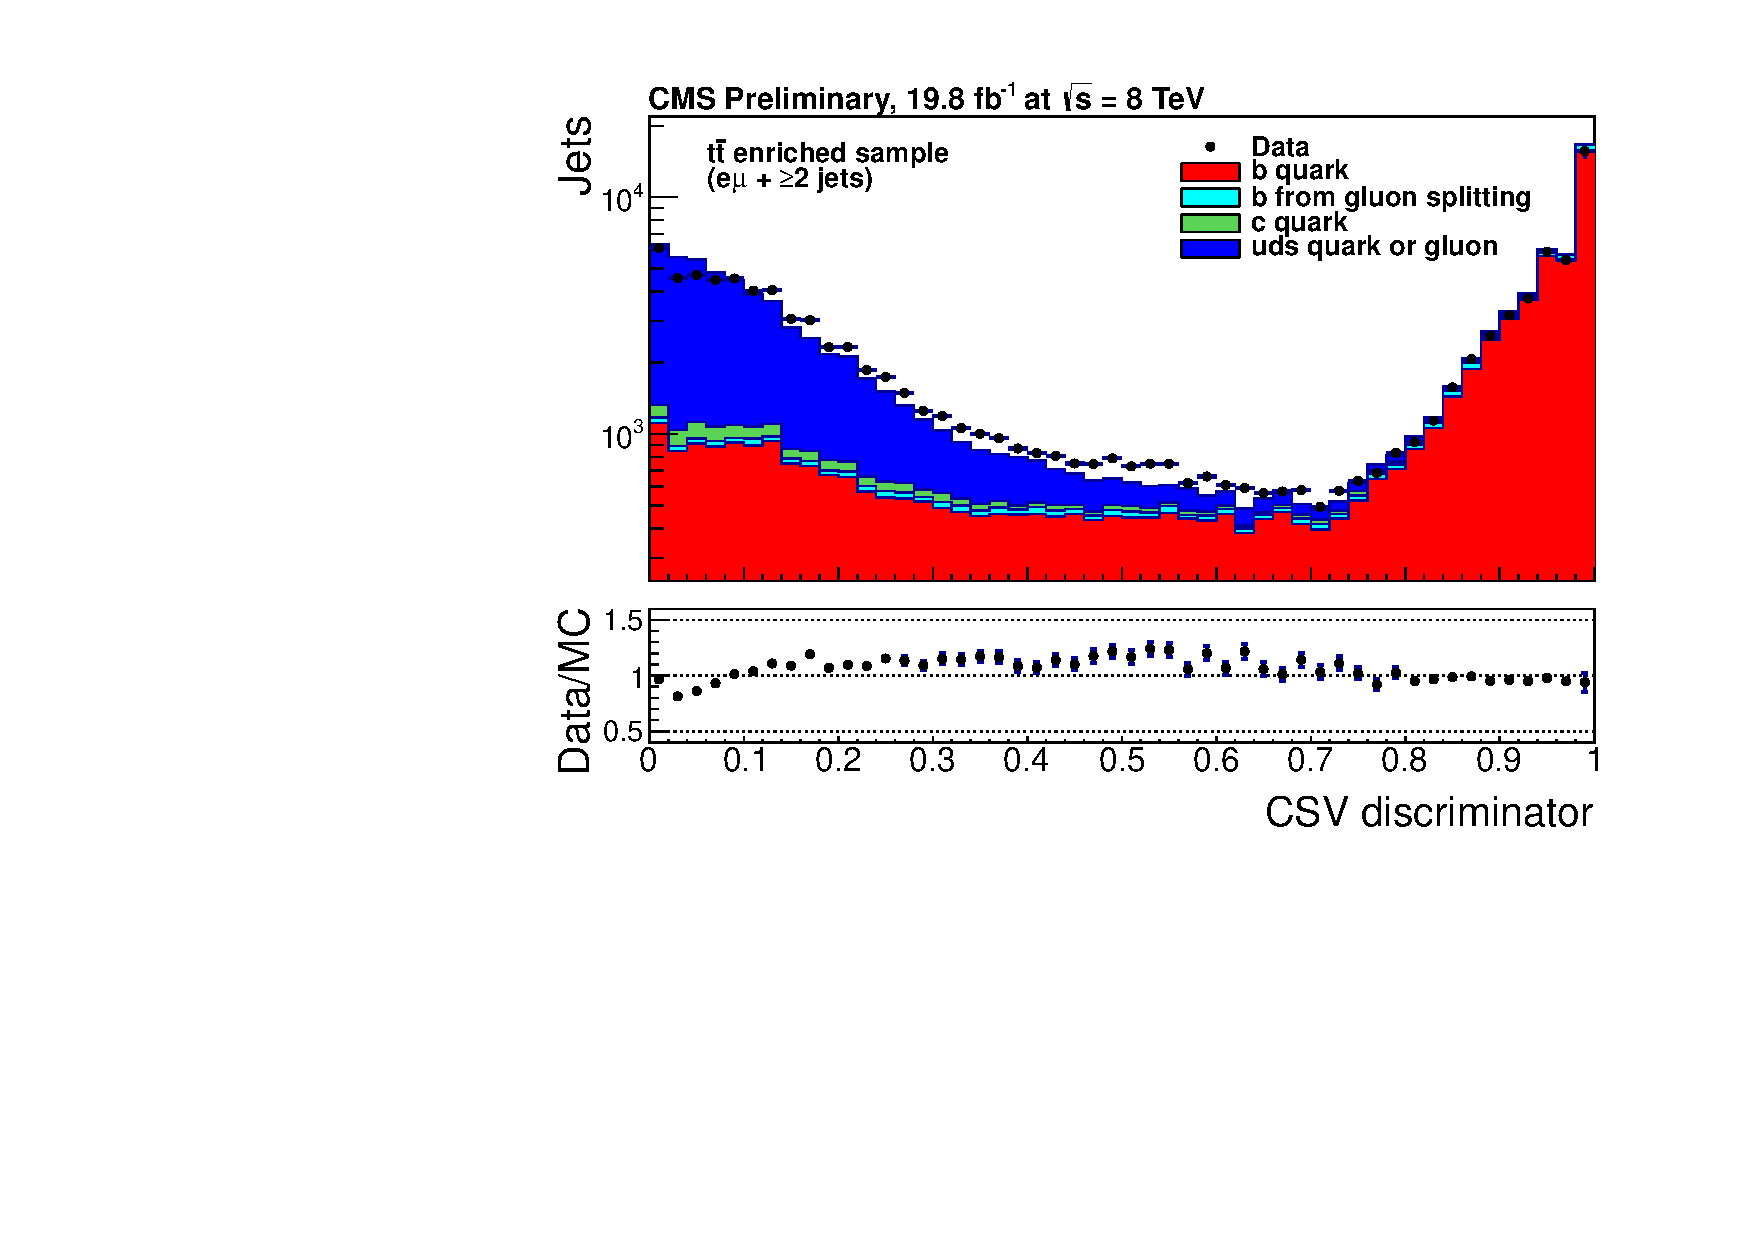
\includegraphics[width = 1.0\linewidth]{plots/btag-ttbardiscrim.pdf}
\end{minipage}
\quad
\begin{minipage}[b]{0.70\linewidth}
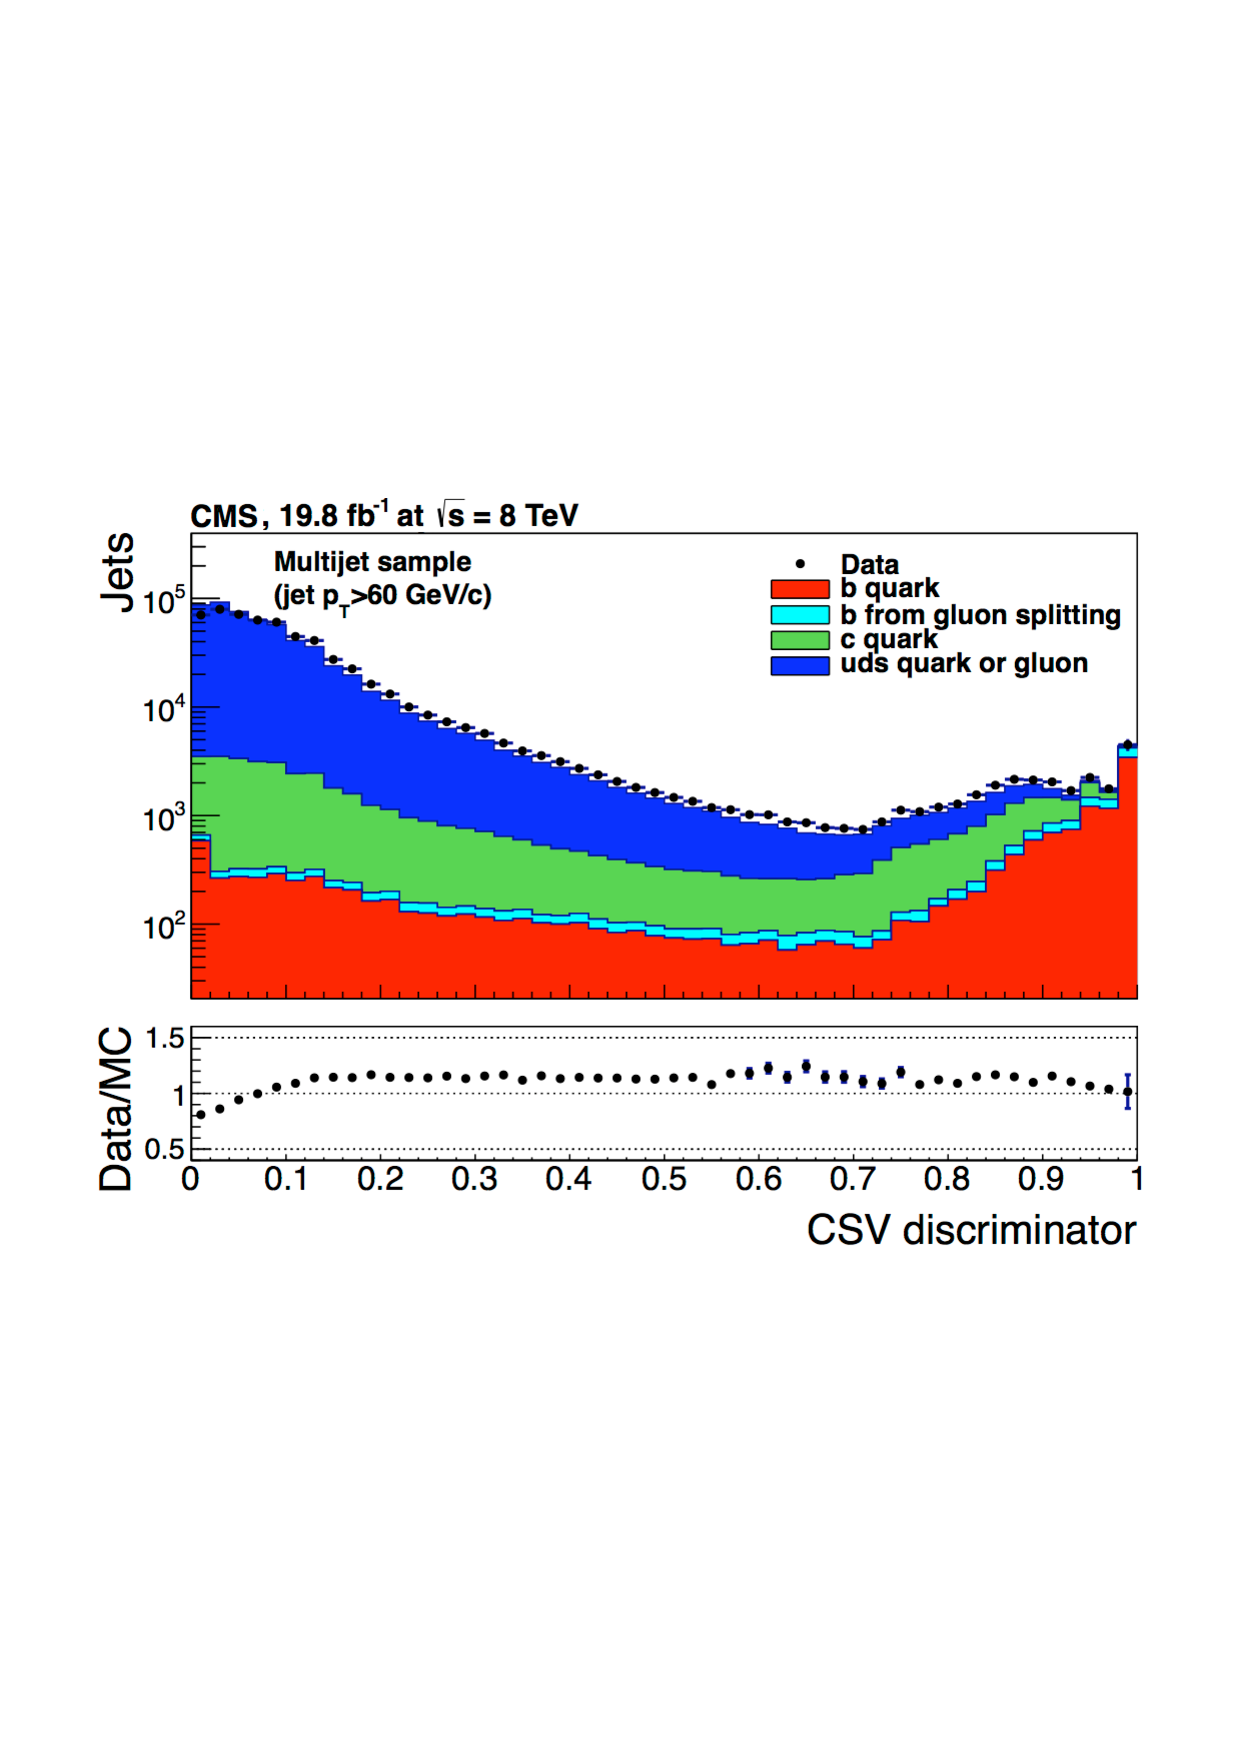
\includegraphics[width = 1.0\linewidth]{plots/btag-multijetdiscrim.pdf}
\end{minipage}
\caption[ \ac{CSV} algorithm discriminator values in enriched ttbar and inclusive multi-jet samples]{\ac{CSV}algorithm discriminator values in enriched ttbar (top) and inclusive multi-jet samples (bottom) for b,c and light flavoured jets. The discriminator value used for each working points are determined from the misidentification probability for light-parton jets to be tagged as a b-jet, which are given as 0.244 (10\%), 0.679 (1\%) and 0.898 (0.1\%) for the L, M and T working points respectively. }
\label{fig:btagdescrims}
\end{figure}

The b-tagging performance is evaluated to measure the b-jet tagging efficiency \effb, and the misidentification probability of charm \effc and light-parton jets \effs . The tagging efficiencies for each of these three jet flavours are compared between data and MC simulation, from which a series of $\pt$ and $\lvert\eta\rvert$ binned jet corrections are determined,

\begin{equation}
SF_{b,c,s} = \frac{\epsilon^{data}_{b,c,s}}{\epsilon^{MC}_{b,c,s}} .
\end{equation}

These are collectively named `Btag Scale Factors' and allow MC simulation to accurately reflect the running conditions and performance of the tagging algorithm in data. Understanding of the b-tagging efficiency is essential in order to minimise systematic uncertainties in physics analyses that employ b-tagging. \\
 
The b-tagging efficiency is measured in data using several methods applied to multi-jet events, primarily based on a sample of jets enriched in heavy flavour content. One method requires the collection of events with a poorly isolated muon within a cone $\Delta R < 0.4$ around the jet axis. Due to the semi-leptonic branching fraction of b hadrons is significantly larger than that for other hadrons, these jets are more likely to arise from b quarks than from another flavour. The resultant momentum component of the muon, transverse to the jet axis, is larger in b-hadron decays than from light or charm flavoured jets.  Additionally, the performance of the tagger can also be benchmarked in \ttbar events, where the top quark is expected to decay to a W boson and a b quark about 99.8$\%$ of the time \cite{pdg2012}. Further selection criteria is applied to these events to further enrich the b quark content of these events. The methods to identify b-jets in data are discussed in great detail at \cite{btag7tev}. The jet flavours are determined in simulation using truth level information and are compared to data to determine the correction scale factors ($SF_{b}$). These are displayed for the \ac{CSVM} tagger in Figure \ref{fig:btagscalefactors}. 

\begin{figure}[ht]
\centering
\begin{minipage}[b]{0.31 \linewidth}
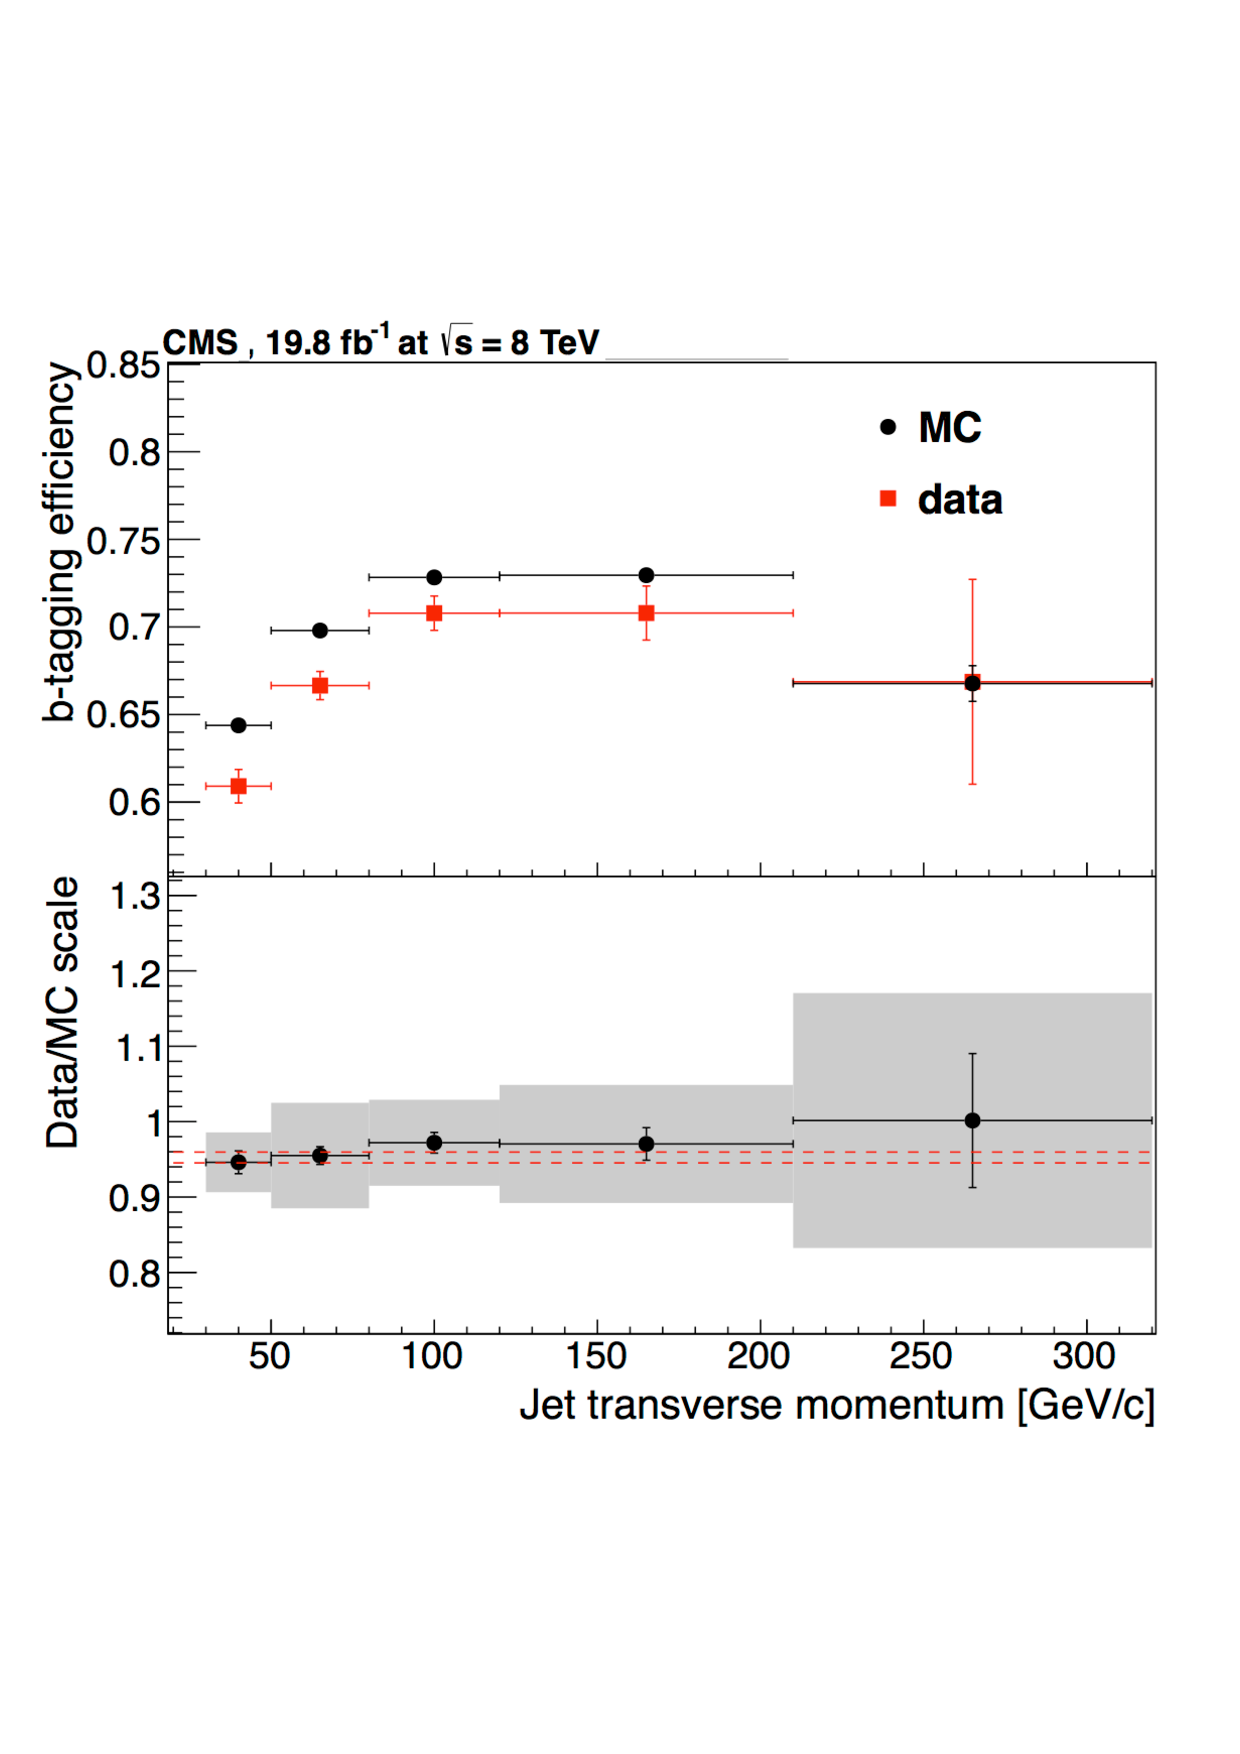
\includegraphics[width = 1.0\linewidth]{plots/btag-csvm_pt_sf.pdf}
\end{minipage}
\quad
\begin{minipage}[b]{0.31\linewidth}
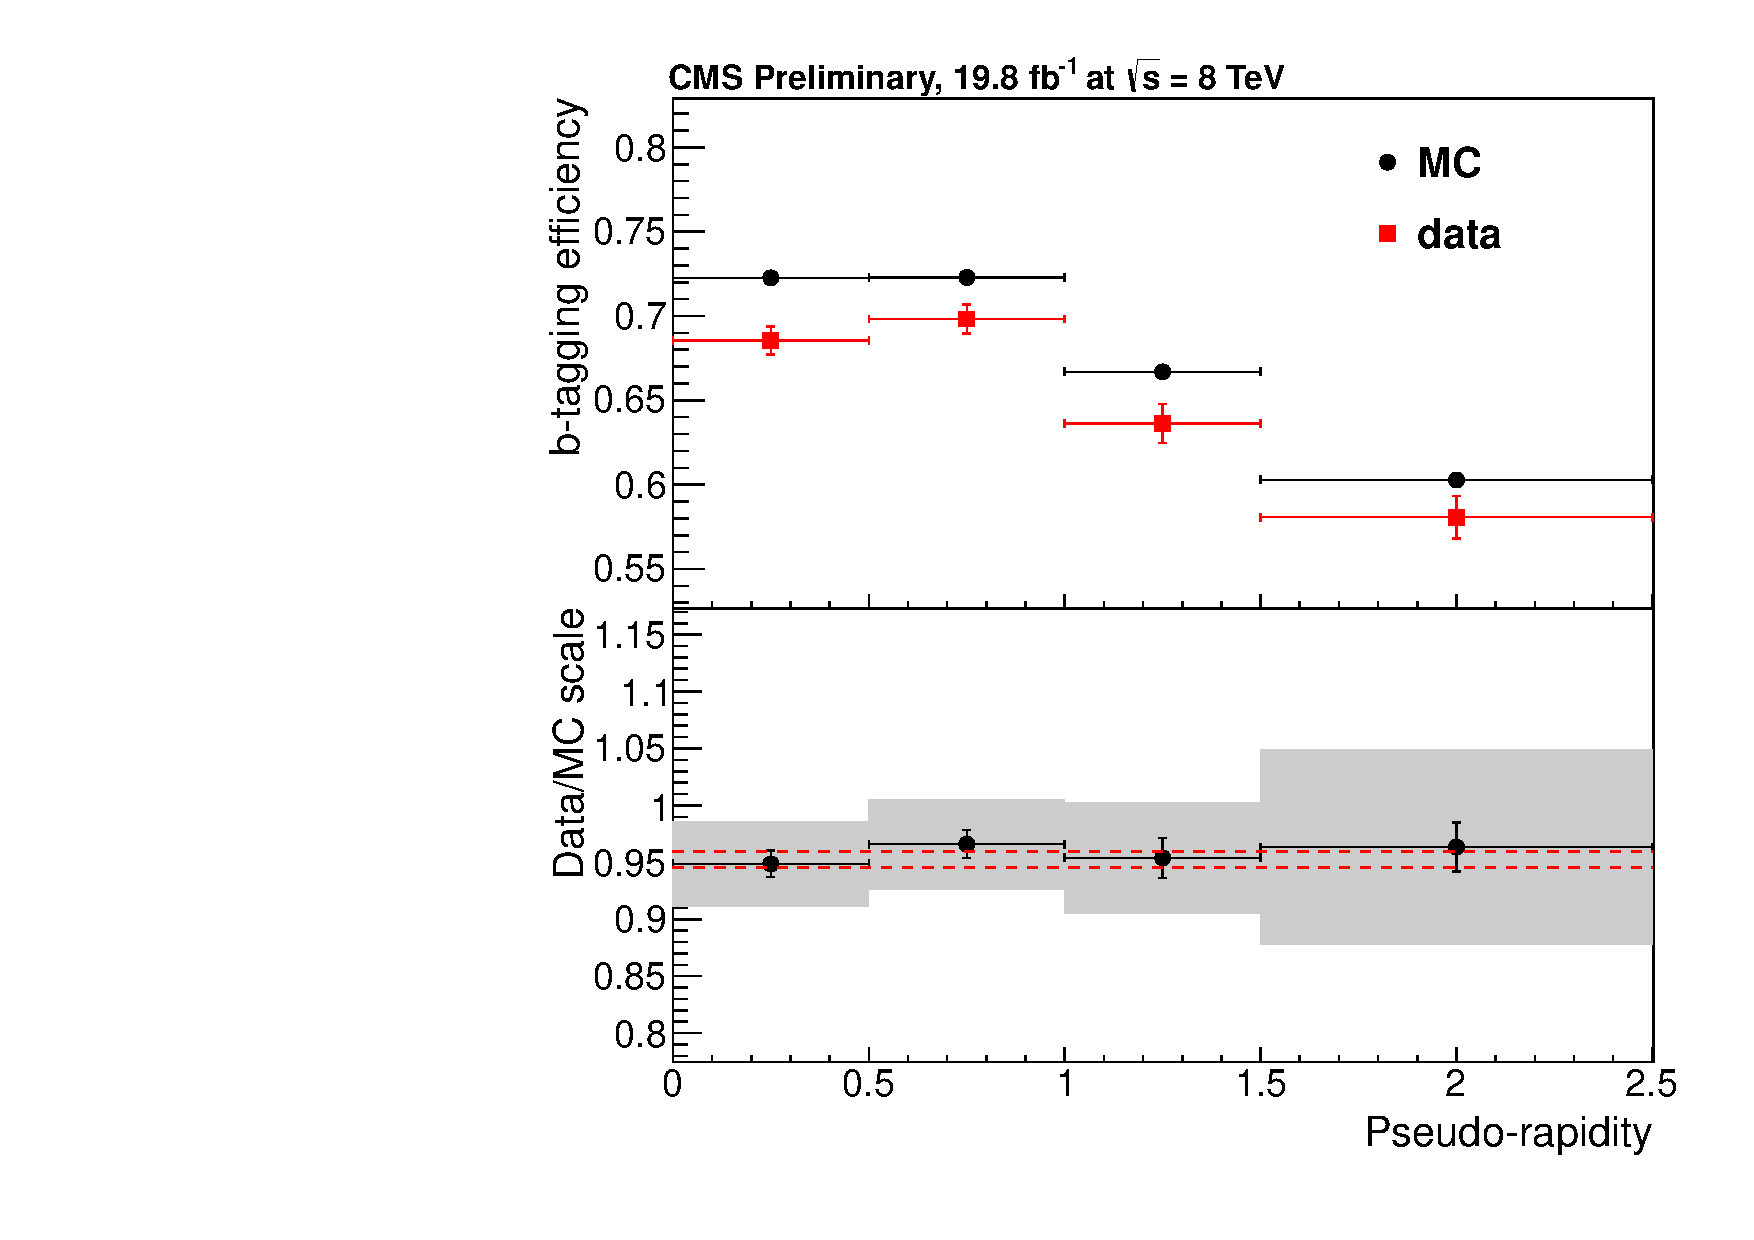
\includegraphics[width = 1.0\linewidth]{plots/btag-csvm_eta_sf.pdf}
\end{minipage}
\quad
\begin{minipage}[b]{0.31\linewidth}
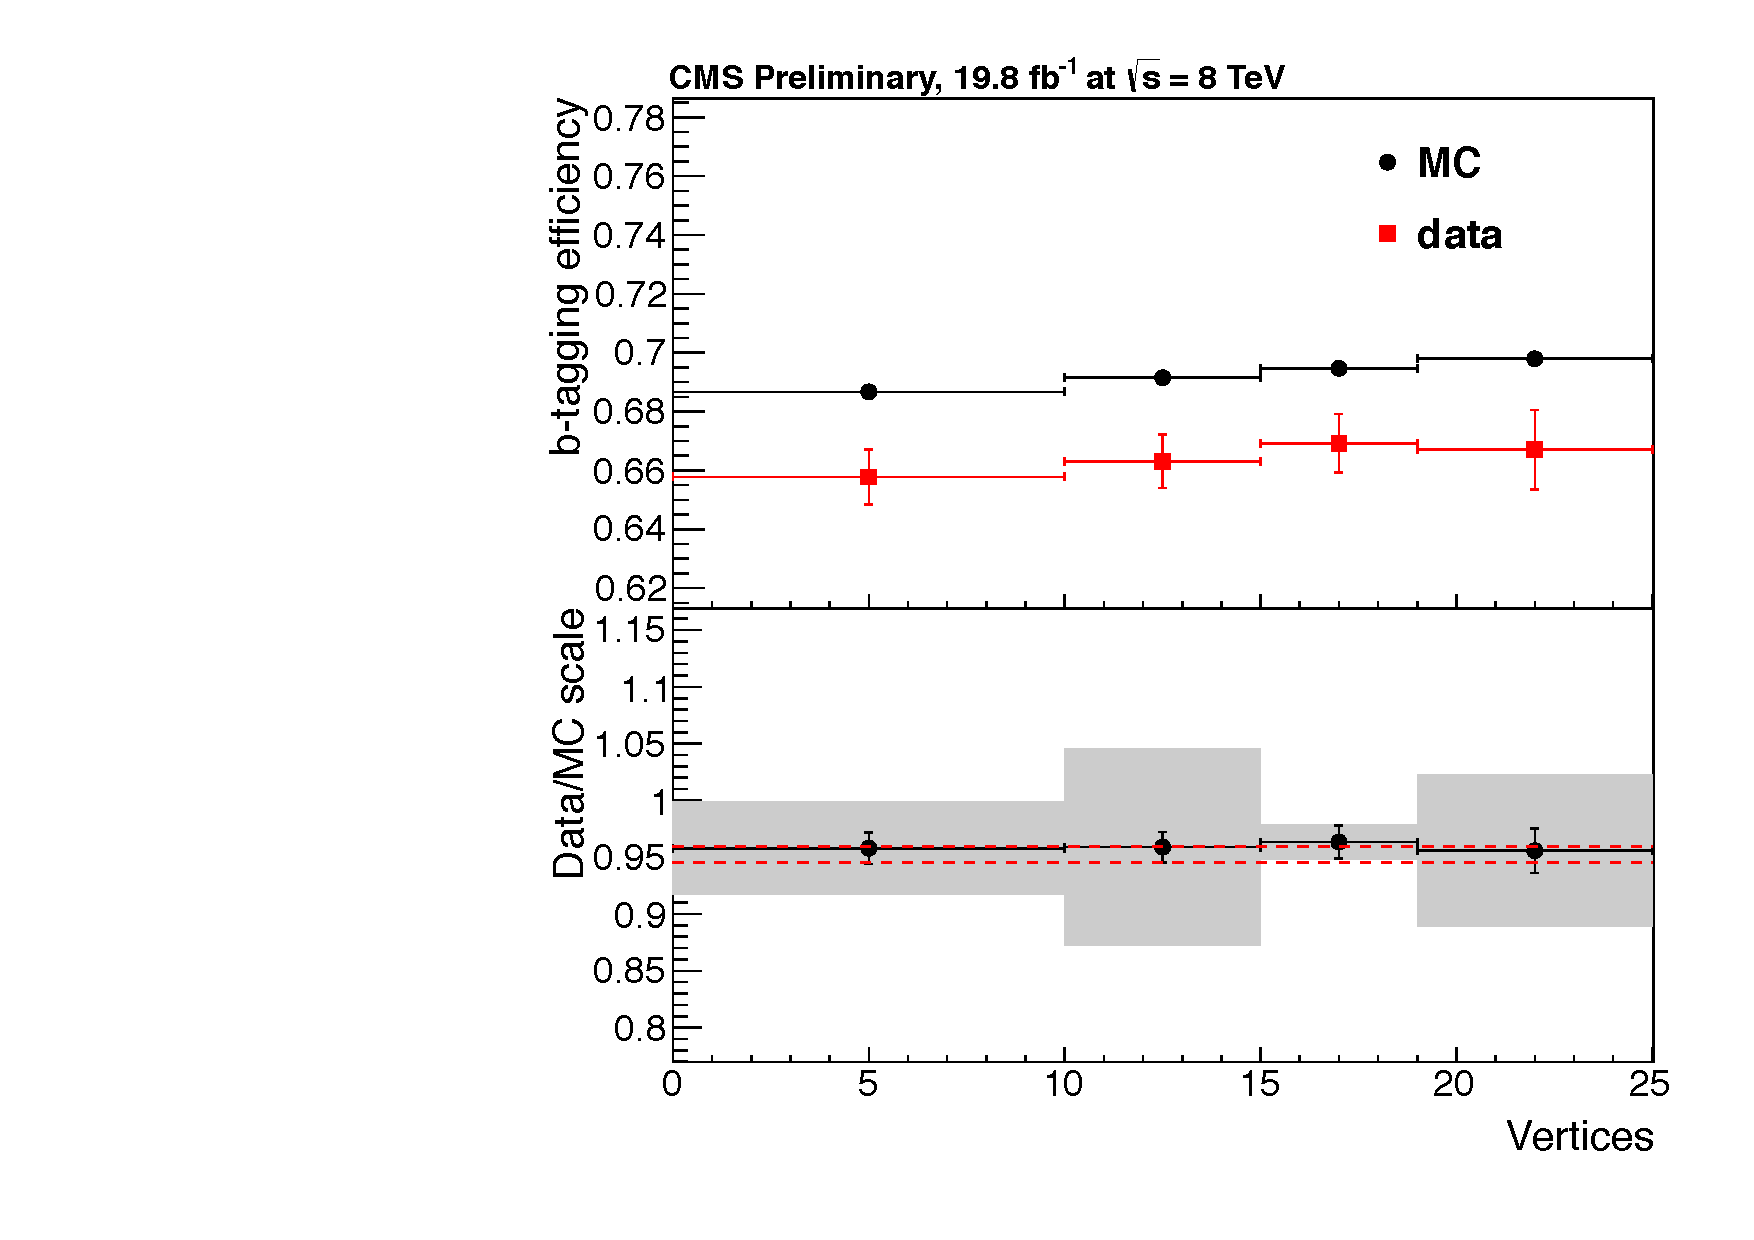
\includegraphics[width = 1.0\linewidth]{plots/btag-csvm_vert_sf.pdf}
\end{minipage}
\caption[Data/MC b-tag scale factors derived using the \ac{CSVM} tagger.]{Measured in \ttbar $\rightarrow$ di-lepton events using the \ac{CSVM} tagger: (upper panels) b-tagging efficiencies and (lower panels) data/MC scale factor $SF_{b}$ as a function of (left) jet $\pt$, (middle) jet $\lvert\eta\rvert$ and (right) number of primary vertices. In the lower panels, the grey filled areas represent the total statistical and systematic uncertainties, whereas the dotted lines are the average $SF_{b}$ values within statistical uncertainties.}
\label{fig:btagscalefactors}
\end{figure}

The measurement of the misidenti�cation probability for light-parton jets relies on the inversion of tagging algorithms, selecting non-b jets using the same variables and techniques used in benchmarking the b-tagging efficiency. The scale factors ($SF_{s}$) to be applied to MC are shown in Figure \ref{fig:mistagscalefactors} for the \ac{CSVM} tagger.

\begin{figure}[ht]
\centering
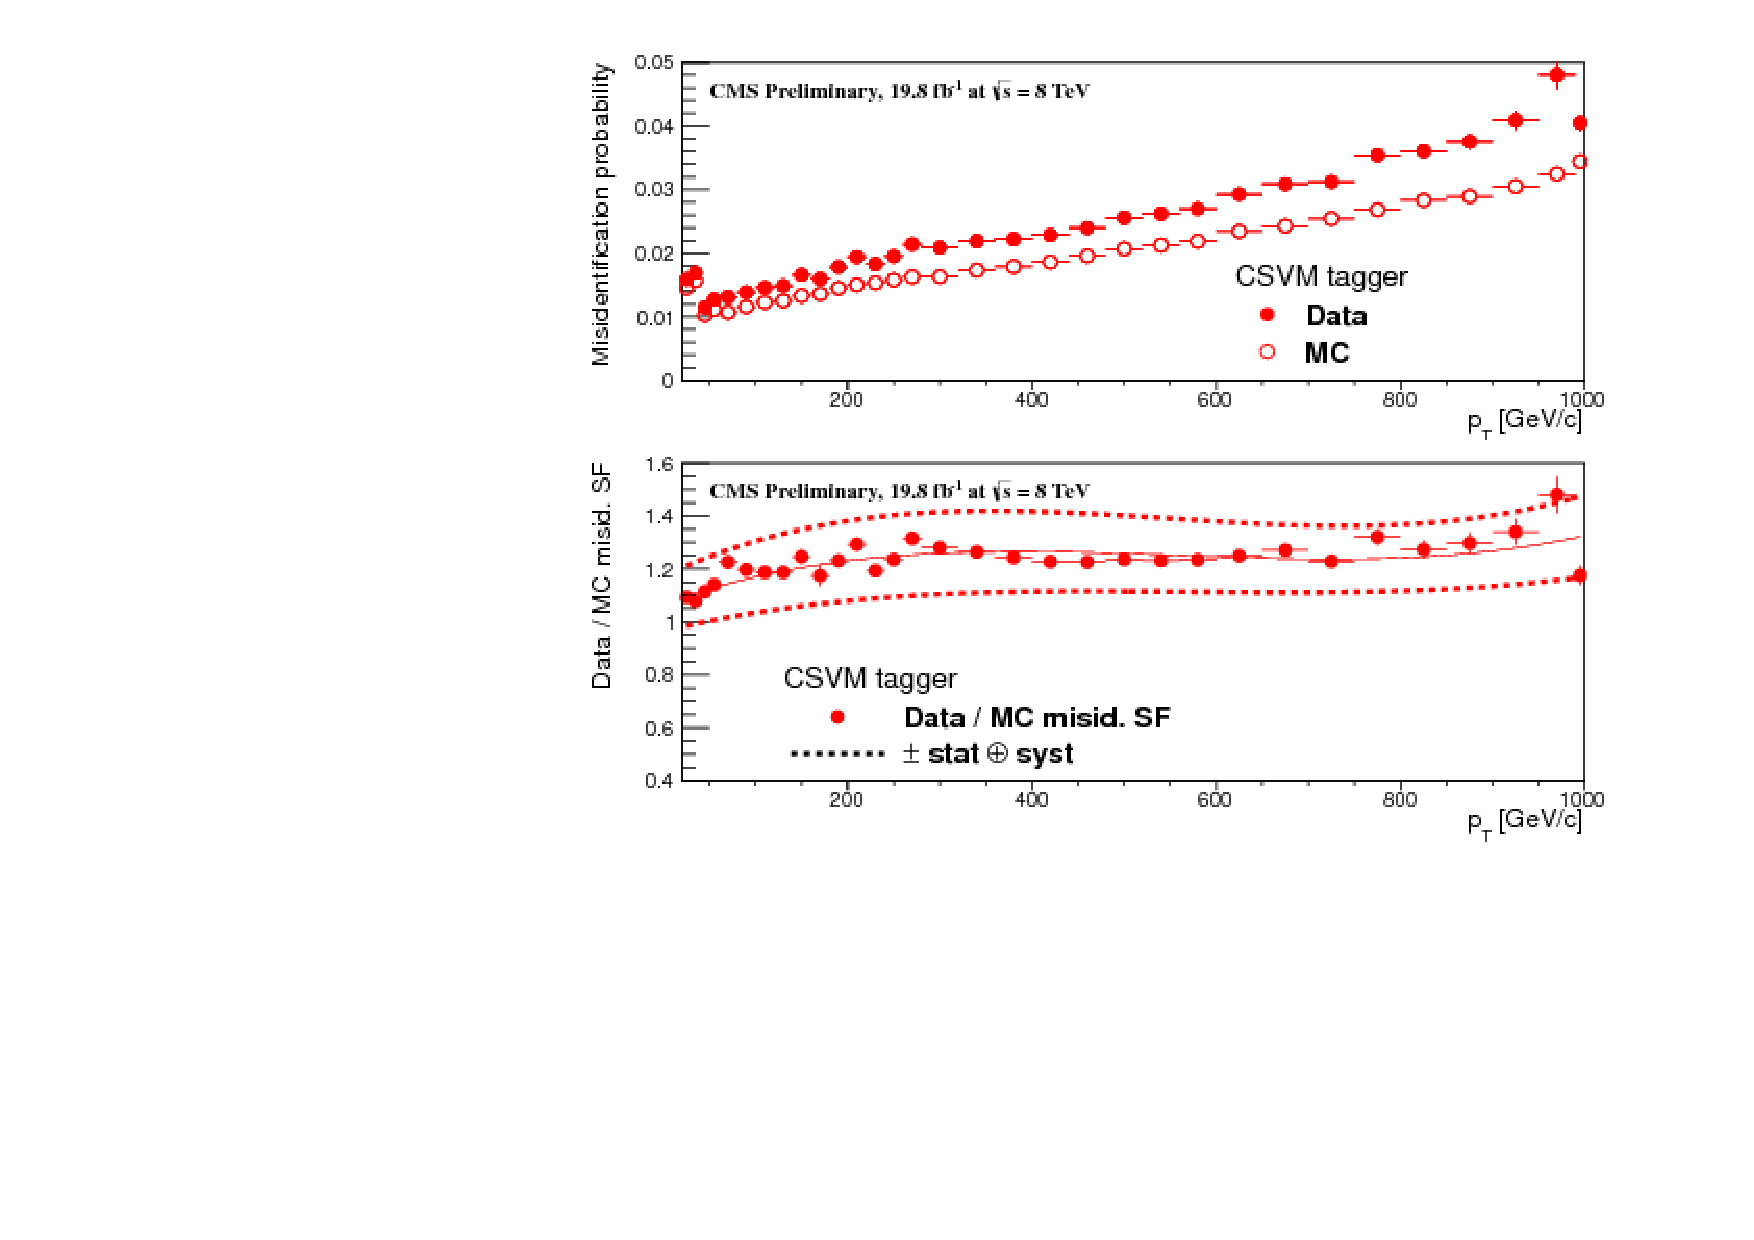
\includegraphics[width=0.70\linewidth]{plots/btag-csvmsf_v2.pdf}
\caption[Data/MC mis-tag scale factors derived using the \ac{CSVM} tagger.]{For the \ac{CSVM} tagging criterion: (top) misidenti�cation probability in data (filled circles) and simulation (open circles); (bottom) scale factor for the misidenti�cation probability. The last $\pt$ bin in each plot includes all jets with $\pt > 1000$ \GeV. The solid curve is the result of a polynomial fit to the data points. The dashed curves represent the overall statistical and systematic uncertainties on the measurements.}  

\label{fig:mistagscalefactors}
\end{figure}


\section{Triggering System}

\label{sec:triggersystem}

With bunch crossings separated by just 50 ns, the rate at which data from all collisions would have to be written out and processed would be unfeasible. A two-tiered triggering system is applied at \ac{CMS} in order to cope with the high collision rate of protons. The \ac{CMS} trigger is designed to use limited information from each event to determine whether to record the event, reducing the rate of data taking to manageable levels whilst ensuring a high efficiency of interesting physics object events are selected.

The \ac{L1} is a pipelined, dead-timeless system based on custom-built electronics \cite{Dasu:2000ge}, and is a combination of several sub systems which is shown pictorially in Figure \ref{fig:l1triggersystem}. The \L1 system is covered in more detail within the following section, along with a description of the service work undertaken by the author to benchmark the performance of the \L1 calorimeter trigger during the 2012 8 \TeV run period.


\begin{figure}[ht]
\centering
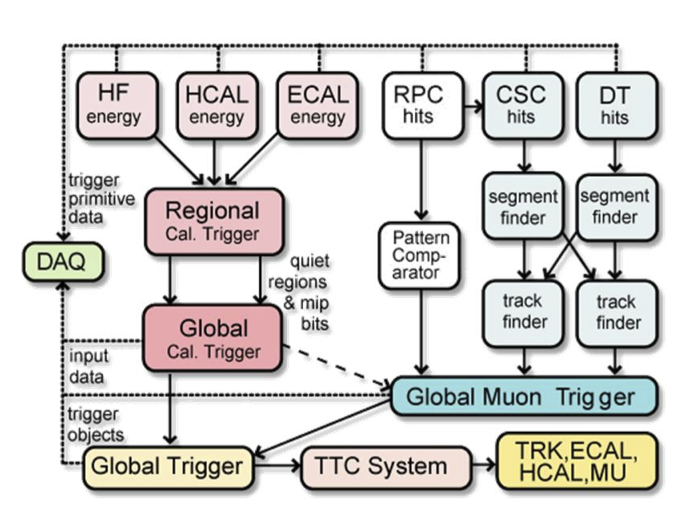
\includegraphics[width=0.80\textwidth]{plots/l1triggersystem.pdf}
\caption[The \ac{CMS} \ac{L1} Trigger system.]{The \ac{CMS} \ac{L1} Trigger system.}  
\label{fig:l1triggersystem}
\end{figure}



The \acf{HLT} is a large farm of commercial computers \cite{Sphicas:2002gg}. The \ac{HLT} processes events with software reconstruction algorithms that are more detailed, giving performance more similar to the reconstruction used offline. The \ac{HLT} reduces the event rate written to disk by a factor of $\sim$ 500 ($\sim$200Hz). The recorded events are transferred from \ac{CMS} to the \ac{CERN} computing centre, where event reconstruction is performed, and then distributed to \ac{CMS} computing sites around the globe for storage and analysis.

\subsection{The Level-1 Trigger}
\label{subsec:l1trigger}

The \L1 trigger reduces the rate of events collected from 40 MHz to $\sim$100 kHz using information from just the calorimeters and muon chambers, but not the tracker. This is due to requirement that data from each and every bunch crossing be analysed with no dead time, drastically reducing time available to process and reconstruct objects in making a trigger decision. This facilitates the need for a pipelined processing architecture, and so a tree system of triggers is used to decide whether to pass on an event to the \ac{HLT} for further reconstruction.
 
Calorimeter and muon event information is processed separately by the \acf{RCT} and \acf{RMT} systems respectively. 

Within the \ac{RCT}, energy deposits from trigger towers in the \ac{ECAL} and \ac{HCAL} calorimeters are summed into coarser calorimeter regions and sent to the \acf{GCT} for jet clustering.

Given that electron and photon are much narrower objects than jets, the \ac{RCT} is used to identify these candidates but makes no attempt to distinguish between them at this stage given the lack of tracking information. They are first identified by ensuring the energy deposits within the central trigger tower and its surrounding cells are above a certain programmable threshold. To ensure the object is not a hadron, the ratio of \ac{HCAL} to \ac{ECAL} in the central tower is calculated and checked to be below 5\%. Additional algorithms are employed to ascertain whether the e/$\gamma$ object is isolated/non-isolated.

In the \L1 \ac{GCT}, coarse measurements of the energy deposited in the electromagnetic and hadronic calorimeters are combined, and by using sophisticated algorithms the following tasks are performed:

\begin{itemize}
	\item isolated and non-isolated electromagnetic objects are sorted (e and $\gamma$), with the four highest ranked (equivalent to highest transverse energy $E_{T}$) objects of each type passed onto the \ac{GT},
	\item energy sums from the calorimeters supplied by the \ac{RCT} are used in performing jet clustering (described in the following section). The clustered jets are then sub-divided into categories depending on their pseudo-rapidity and the result of $\tau$ identi�cation, being classified as either centre, forward, or tau ($\tau$). After being sorted by rank, the four highest of each category are passed to the \ac{GT} for use in trigger decisions,
	\item total transverse energy ($\et$), the scalar sum of the energy deposits measured by L1,  and missing transverse energy ($\met$), defined as the negative vector sum of the transverse energy deposits measured at \L1 are calculated,
	\item total transverse jet energy ($\theht$), the scalar sum of the energy of all L1 clustered jet objects, and missing transverse jet energy ($\mht$), defined as the negative vector sum of the energy from L1 clustered jet objects are calculated and passed to the \ac{GT}. 
\end{itemize}

In addition, quantities suitable for triggering minimum bias events, forward physics and beam background events are determined. Relevant muon isolation information is also passed on to the \ac{GMT} to be used in decisions involving the muon triggers, where it is combined with information from across the three muon sub-systems. The resultant final accept/reject decision at \ac{L1} is then performed by the \ac{GT}, based on the objects received from the \ac{GCT} and \ac{GMT} ($e/\gamma$, $\mu$, jets, $\et$, $\met$, $\theht$, $\mht$).

The \L1 trigger is therefore of upmost importance to the functioning of the detector. Without a high-performing trigger and a good understanding of its performance, there would be no data to analyse. Whilst it would be possible to maintain trigger efficiency by increasing the triggering thresholds for different jet or energy sum quantities, this is far from ideal. This could result in the failure to be sensitive to a wide range of new physics signatures, including many types of compressed spectra \ac{SUSY} models where the mass splitting between squarks/gluinos and the \ac{LSP} is small. 

One such method introduced to help maintain low triggering thresholds, was via the introduction of a jet seed threshold into the \L1 jet clustering algorithm. Observations of how the \L1 trigger performance is affected by both the jet seed threshold, and changing \ac{lhc} running conditions over the 2012 run period is presented in the following Sections (\ref{subsec:l1jettrigger} - \ref{subsec:l1summary}).

\subsection{The \L1 Trigger Jet Algorithm}
\label{subsec:l1jettrigger}

The \L1 jet algorithm clusters jets using the transverse energy sums computed by the calorimeter trigger regions. Each region consists of $4 \times 4 $ trigger tower windows which within the \ac{CMS} barrel spans a region of $\Delta \eta \times \Delta \phi = 0.087 \times 0.087$ in pseudorapidity-azimuth. The jet trigger uses a $3 \times 3$ calorimeter region (144 trigger towers) sliding window technique, as shown on the left of Figure \ref{fig:l1jetalgo}. 

To increase the speed at which jets are clustered, 18 jet finders operate simultaneously over the whole detector. In order to reduce the total data duplicated and shared between these jet finders, the \ac{GCT} employs a pre-clustering algorithm which then only share information with neighbouring regions when clustered jets are found.

A jet candidate is created when the sum of the \ac{HCAL} and \ac{ECAL} energies of the central calorimeter region has an energy deposit larger than all of its neighbouring regions $E_{\text{T central}} > E_{\text{T surround}}$.  During the 2012 run period, a minimum threshold of 5 \GeV was imposed on the central seeding region to suppress noise from non-collimated pile-up jets. This threshold is applied on the raw, uncorrected energy of the trigger regions and affects all clustered \L1 jets. The effect of such a change to the jet algorithm on the triggering performance of L1 quantities is shown in Section (\ref{subsec:l1jetseedpu}).

The \L1 jets are characterised by the $\et$, summed over the $3 \times 3$ calorimeter regions, which corresponds to $12 \times 12$ trigger towers in barrel and endcap, or $3 \times 3$ larger \ac{HF} towers in the \ac{HF}. The $\phi$ size of the jet window is the same everywhere, whilst the $\eta$ binning gets somewhat larger at high $\eta$ due to calorimeter and trigger tower segmentation. The jets are labelled by the $(\eta, \phi)$ indices of the central calorimeter region.                                                                                                                                                  

The \ac{GCT} also determines whether or not a $\tau$-veto bit has been set for each calorimeter region. This depends on whether the energy depositions in up to 4 contiguous trigger towers are below a programmable fraction of the regional $E_{T}$, see Figure \ref{fig:l1jetalgo} (right). These topologies are due to the hadronic decay modes of the $\tau$ containing one or three isolated pions. Any jet candidate that has energy deposits spread throughout the trigger towers in a calorimeter region is likely not from one or three isolated pions and the $\tau$-veto bit is set.

Jets with $3.0<|\eta|<5.0$ are classified as forward jets, whereas those with $|\eta|<3.0$ are classified as either a central or $\tau$-jet depending on the outcome of the setting of the $\tau$-veto bits. The four highest energy central, forward and $\tau$-jets in the calorimeter are further passed through \acf{LUT}s, which apply a programmable $\eta-$dependent jet energy scale correction. Finally these jet objects are passed to the \ac{GT} to make \L1 trigger decisions.

\begin{figure}[ht!]
\centering
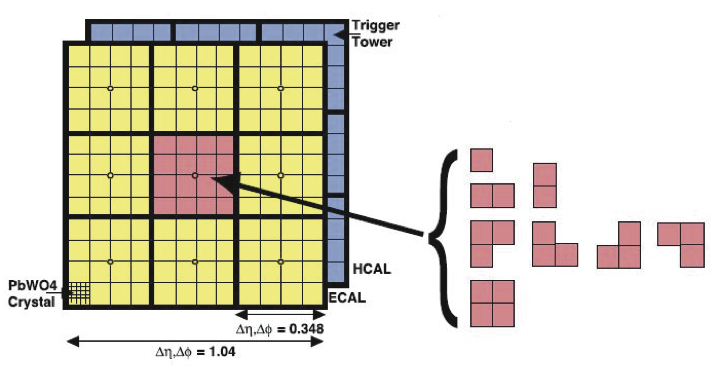
\includegraphics{plots/L1JetAlgorithm.pdf}
\caption[Illustration of the Level-1 jet finding algorithm.]{Illustration of the Level-1 jet finding algorithm. Each cell represents a trigger tower, which is the sum of the transverse energy contributions from both calorimeter systems. The $\tau$-jet veto patterns for the central calorimeter region are displayed on the right.
}  
\label{fig:l1jetalgo}
\end{figure}  

The performance of the \L1 jets is evaluated with respect to offline jets, which are taken from the standard \Calo jet and the \PF jet reconstruction algorithms of \ac{CMS}. Jets are corrected for pile-up and detector effects as described in Section (\ref{subsec:cmsobjects-jets}). A moderate level of noise rejection is applied to the offline jets by selecting jets passing the ``loose'' identification criteria for both \Calo and \PF. These jet criteria are listed in Appendix (\ref{app:jetcriteria}). 


\subsection{Measuring \L1 Jet Trigger Efficiencies}
\label{subsec:l1jettrigeff}

The \L1 jet efficiency is defined as the fraction of leading offline jets which were matched with a L1 $\tau$- or central jet above a certain trigger threshold, divided by all events in the sample with a single offline jet above threshold. 

The efficiency is determined by matching the \L1 and reconstructed offline jets spatially in $\eta - \phi$ space.  This is done by calculating the minimum separation in $\Delta R$ between the highest offline reconstructed jet with $\et > 10$ \GeV and $\lvert\eta\rvert<3$ and any \L1 jet. A match is found when $\Delta R < 0.5$. Should more than one jet satisfy this condition, the jet closest in $\Delta R$ is taken as the matched jet. The matching efficiency for this procedure is found to be close to 100$\%$ above an offline jet threshold of 30(45) GeV for the run 2012B(C) data taking period (see Appendix \ref{app:jetmatching}).

Each efficiency curve is fitted with a function which is the cumulative distribution function of an \acf{EMG} distribution:
\begin{eqnarray}
f(x; \mu, \sigma, \lambda) = \frac{\lambda}{2} \cdot e^{\frac{\lambda}{2}(2 \mu + \lambda \sigma^2 - 2 x)} \cdot \textrm{erfc}\left( \frac{\mu + \lambda \sigma^2 - x}{\sqrt{2} \sigma}\right)
\label{eq:emg}
\end{eqnarray}
where \textrm{erfc} is the complementary error function defined as:
$$ \textrm{erfc}(x) = 1 - \textrm{erf}(x) = \frac{2}{\sqrt{\pi}} \int_{x}^{\infty} e^{-t^2} dt.$$

In this functional form, the parameter $\mu$ determines the point of 50\% of the plateau efficiency, and the $\sigma$ gives the resolution. This parametrisation is used to benchmark the efficiency at the plateau, the turn-on points and resolution for each L1 Jet trigger. The choice of function is purely empirical. Previous studies used the error function alone, which described the data well at high threshold values but could not describe the efficiencies well at lower thresholds \cite{L1JEC}.

The efficiency turn-on curves for various \L1 jet thresholds are evaluated as a function of the offline reconstructed jet E$_{T}$ for central jets with $| \eta | < 3$. These are measured using single isolated $\mu$ triggers which have high statistics, and are orthogonal and therefore unbiased to the hadronic triggers under study. Events are selected with some loose detector based isolation requirements to make sure the muon does not overlap with a jet, causing a discrepancy in the measurement of the calorimetric energy.

The efficiency is calculated with respect to offline \Calo and \PF Jets in Figure  \ref{fig:l1jet-calopf-mu}. Table \ref{tab:l1jettable} shows the values of these parameters, calculated for three example \L1 single jet triggers taken from 2012 8 \TeV data.

\begin{figure}[ht]
\centering
\begin{minipage}[b]{0.48 \linewidth}
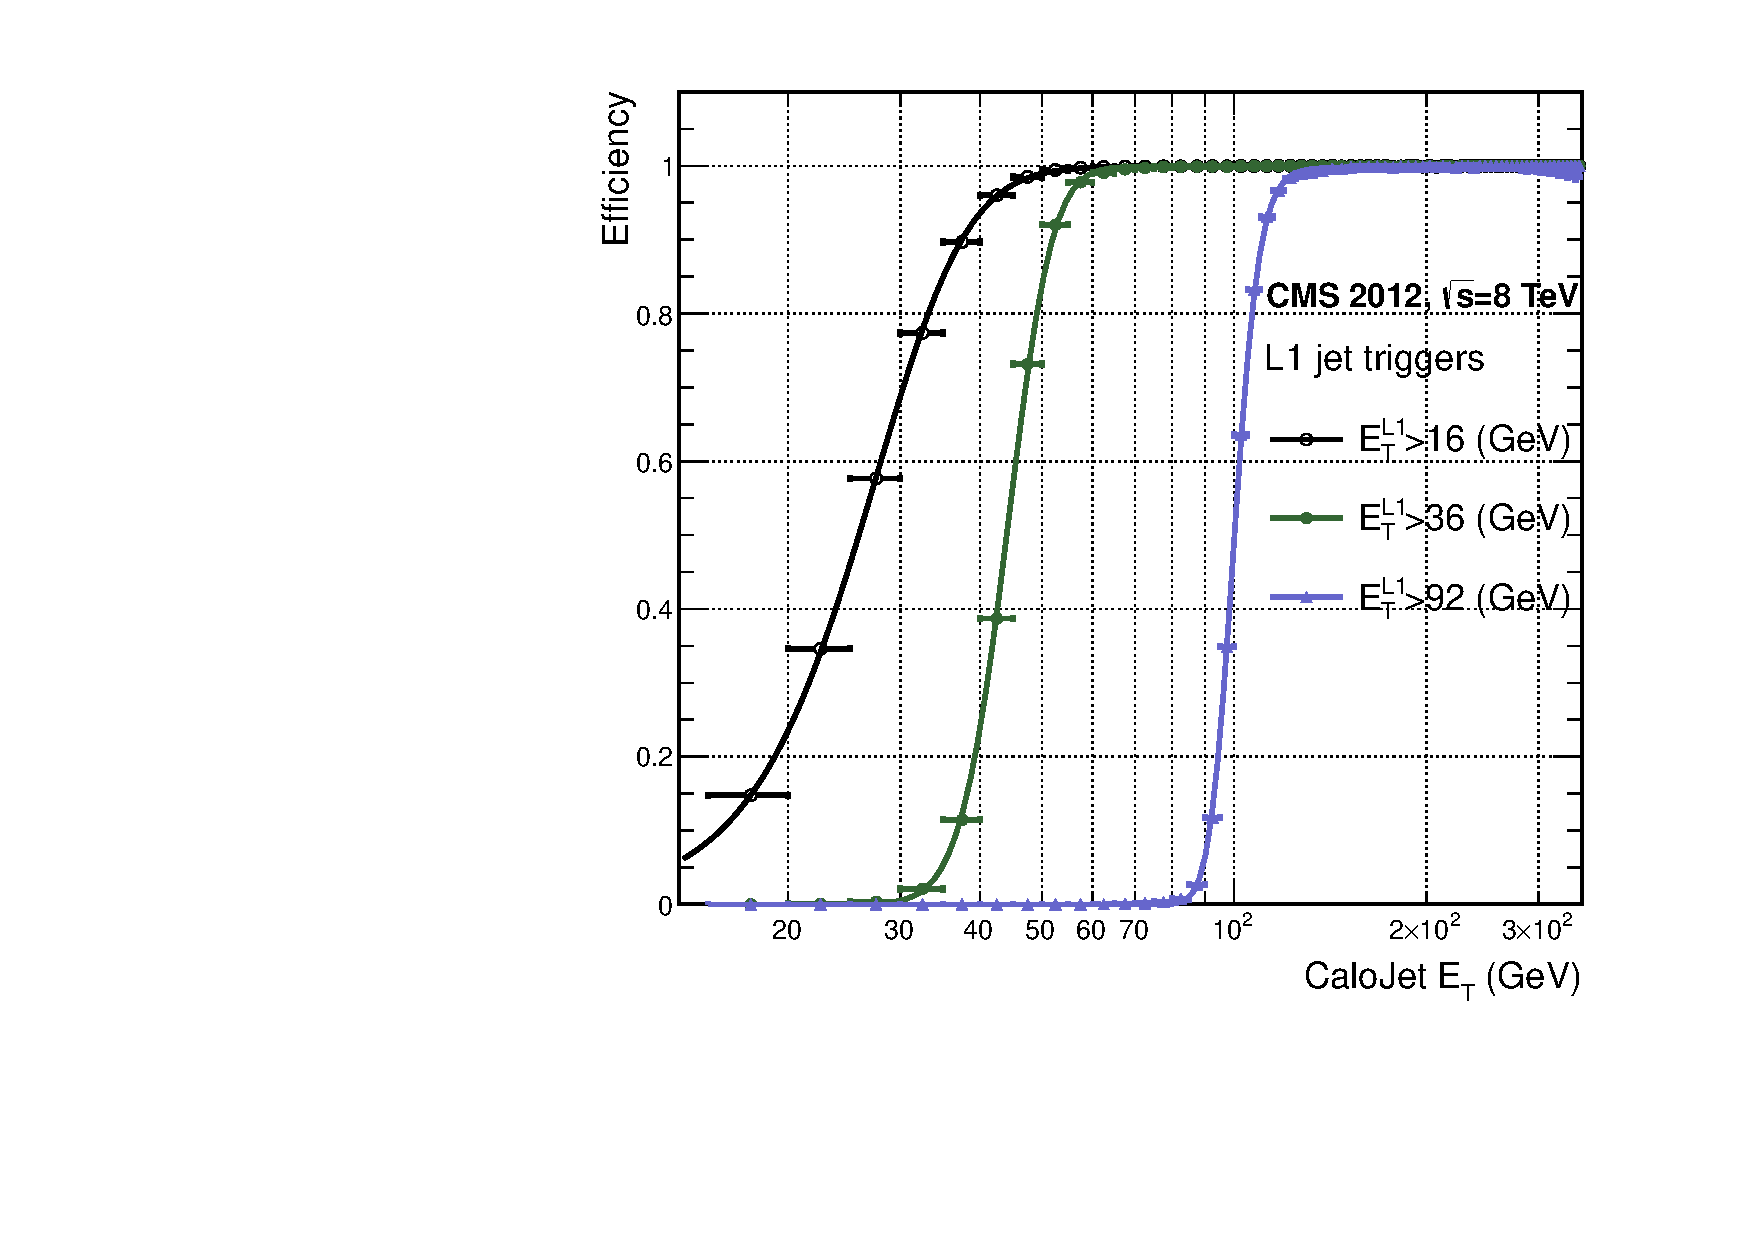
\includegraphics[width = 1.0\linewidth]{plots/jetpt_RunC.pdf}
\end{minipage}
\quad
\begin{minipage}[b]{0.48 \linewidth}
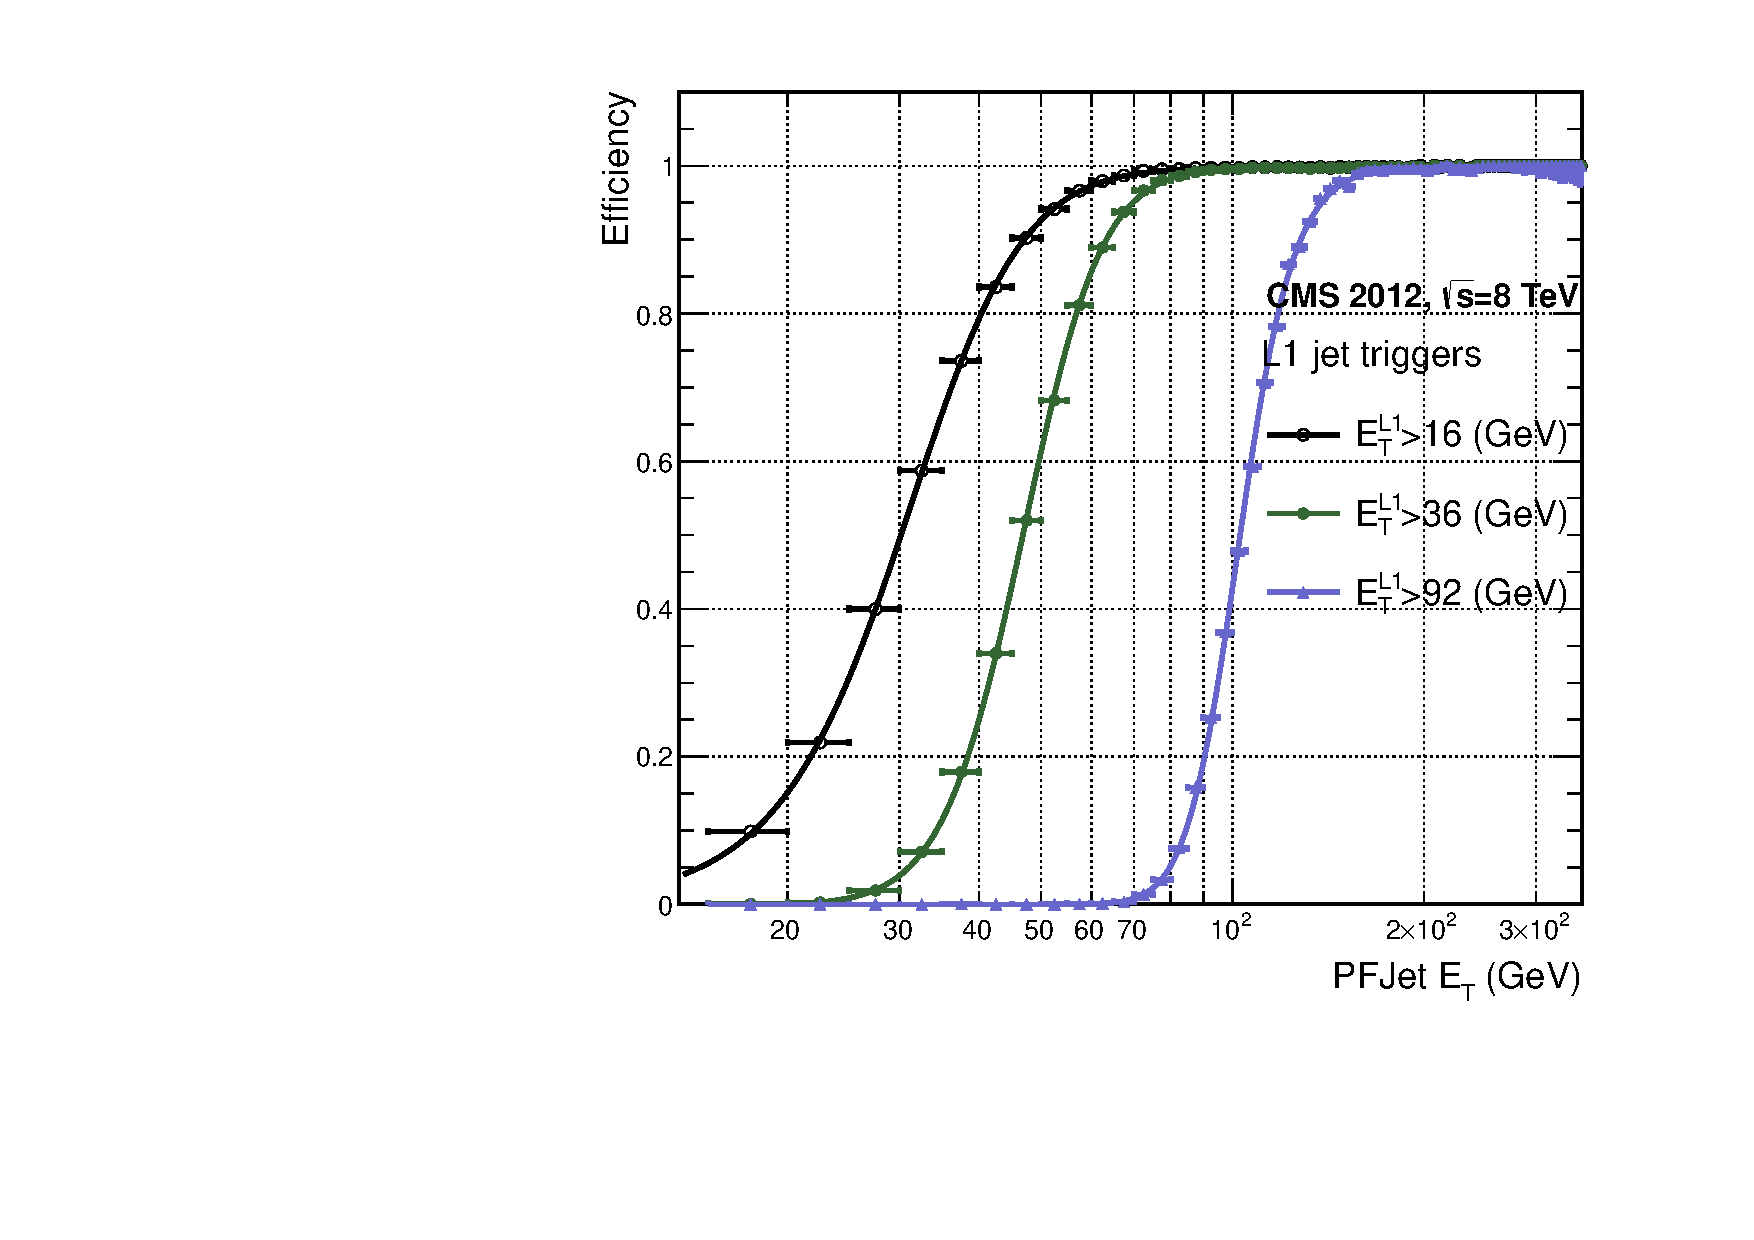
\includegraphics[width = 1.0\linewidth]{plots/jetpt_RunC_PF.pdf}
\end{minipage}
\quad
\caption[L1 jet efficiency turn-on curves as a function of the offline CaloJet and PFJet $\et$. ]{L1 jet efficiency turn-on curves as a function of the offline CaloJet $\et$ (left) and PFJet $\et$ (right), measured in 2012 Run Period C data and collected with an isolated single $\mu$ data sample.}
\label{fig:l1jet-calopf-mu} 

\end{figure}

\begin{table}
\begin{center}
\footnotesize
\begin{tabular*}{0.75\textwidth}{@{\extracolsep{\fill}}c|cc|cc}
\hline
\multicolumn{1}{c}{}& \multicolumn{2}{c}{Calo} & \multicolumn{2}{c}{PF} \\ 
\multicolumn{1}{c}{Trigger} & $\mu$ & \multicolumn{1}{c}{$\sigma$} & $\mu$ & $\sigma$ \\ \hline\hline
L1\_SingleJet16 & 21.09 $\pm$ 0.03 & 7.01 $\pm$ 0.02 & 22.17 $\pm$ 0.04 & 7.83 $\pm$ 0.03 \\ 
L1\_SingleJet36 & 41.15 $\pm$ 0.05 & 5.11 $\pm$ 0.02 & 39.16 $\pm$ 0.06 & 8.04 $\pm$ 0.03 \\ 
L1\_SingleJet92 & 95.36 $\pm$ 0.13 & 5.62 $\pm$ 0.03 & 90.85 $\pm$ 0.19 & 11.30 $\pm$ 0.10  \\ 
\end{tabular*}
\end{center}

\caption[Results of a cumulative \ac{EMG} function fit to the turn-on curves for \L1 single jet triggers in 2012 Run Period C.]{Results of a cumulative \ac{EMG} function fit to the turn-on curves for \L1 single jet triggers in run 2012 Run Period C, measured in an isolated $\mu$ data sample. The turn-on point, $\mu$, and resolution, $\sigma$, of the L1 jet triggers are measured with respect to offline Calo Jets (left) and PF Jets (right). }
\label{tab:l1jettable}
\end{table}

The results from the \L1 single jet triggers shows good performance for both \Calo and \PF jets. A better resolution is observed for \Calo jets with respect to \L1 jet quantities. This effect is due to \Calo jet reconstruction using the same detector subsystems as for \L1 jets. In contrast the \PF jet reconstruction algorithm additionally utilises tracker and muon information, resulting in a poorer resolution when directly compared to \L1 jet objects. 

\subsection{Effects of the \L1 Jet Seed}
\label{subsec:l1jetseedpu}

Between run period B and C of the 2012 data taking period, a jet seed threshold was introduced into the \L1 jet clustering algorithm. There was previously no direct requirement made on the energy deposited in the central region. 

The introduction of a jet seed threshold required that the central region have an uncorrected energy deposit of $\et \geq 5$ \GeV. This value was motivated by studies of the effect that different jet seed thresholds had upon the trigger cross-sections and efficiencies of various \theht, single jet and multi-jet triggers. It was found that the 5 \GeV threshold gave large reductions in trigger cross-sections (particularly in the case of multi-jet and \theht triggers), whilst having a small impact on the measured efficiencies of these triggers \cite{Shorney-Mathias:1641954}.

Its main purpose was to counteract the effects of high pile up running conditions which create a large number of soft non-collimated jets, that are then added to the jets from the primary interaction or other soft jets from other secondary interactions \cite{L1bryn}. This in turn causes a large increase in trigger rate, due to the increase in the likelihood that the event causes the \L1 trigger to fire. 

The effect of the introduction of this jet seed threshold between these two run periods is benchmarked through a comparison of the efficiency of the \L1 jet triggers with respect to offline Calo jets and is shown in Figure \ref{fig:l1jetseeds}. The \L1 $H_{T}$ trigger efficiency is also measured and is shown in Figure \ref{fig:l1jetseedht}. The \L1 \theht sum is compared against the offline $\theht$ constructed from Calo jets with $\et \geq$ 40 \GeV. This requirement is imposed to account for the relative difference between uncorrected jet energy deposits within the \ac{GCT} used to calculate the \L1 \theht sum, and those same deposits after full object reconstruction has occurred.

To negate any effects from different pile-up conditions in the run periods, the efficiencies are measured in events which contain between 15 and 20 primary vertices, as defined in Appendix (\ref{app:primaryvertices}). 

\begin{figure}[ht]
\centering
\begin{minipage}[b]{0.48 \linewidth}
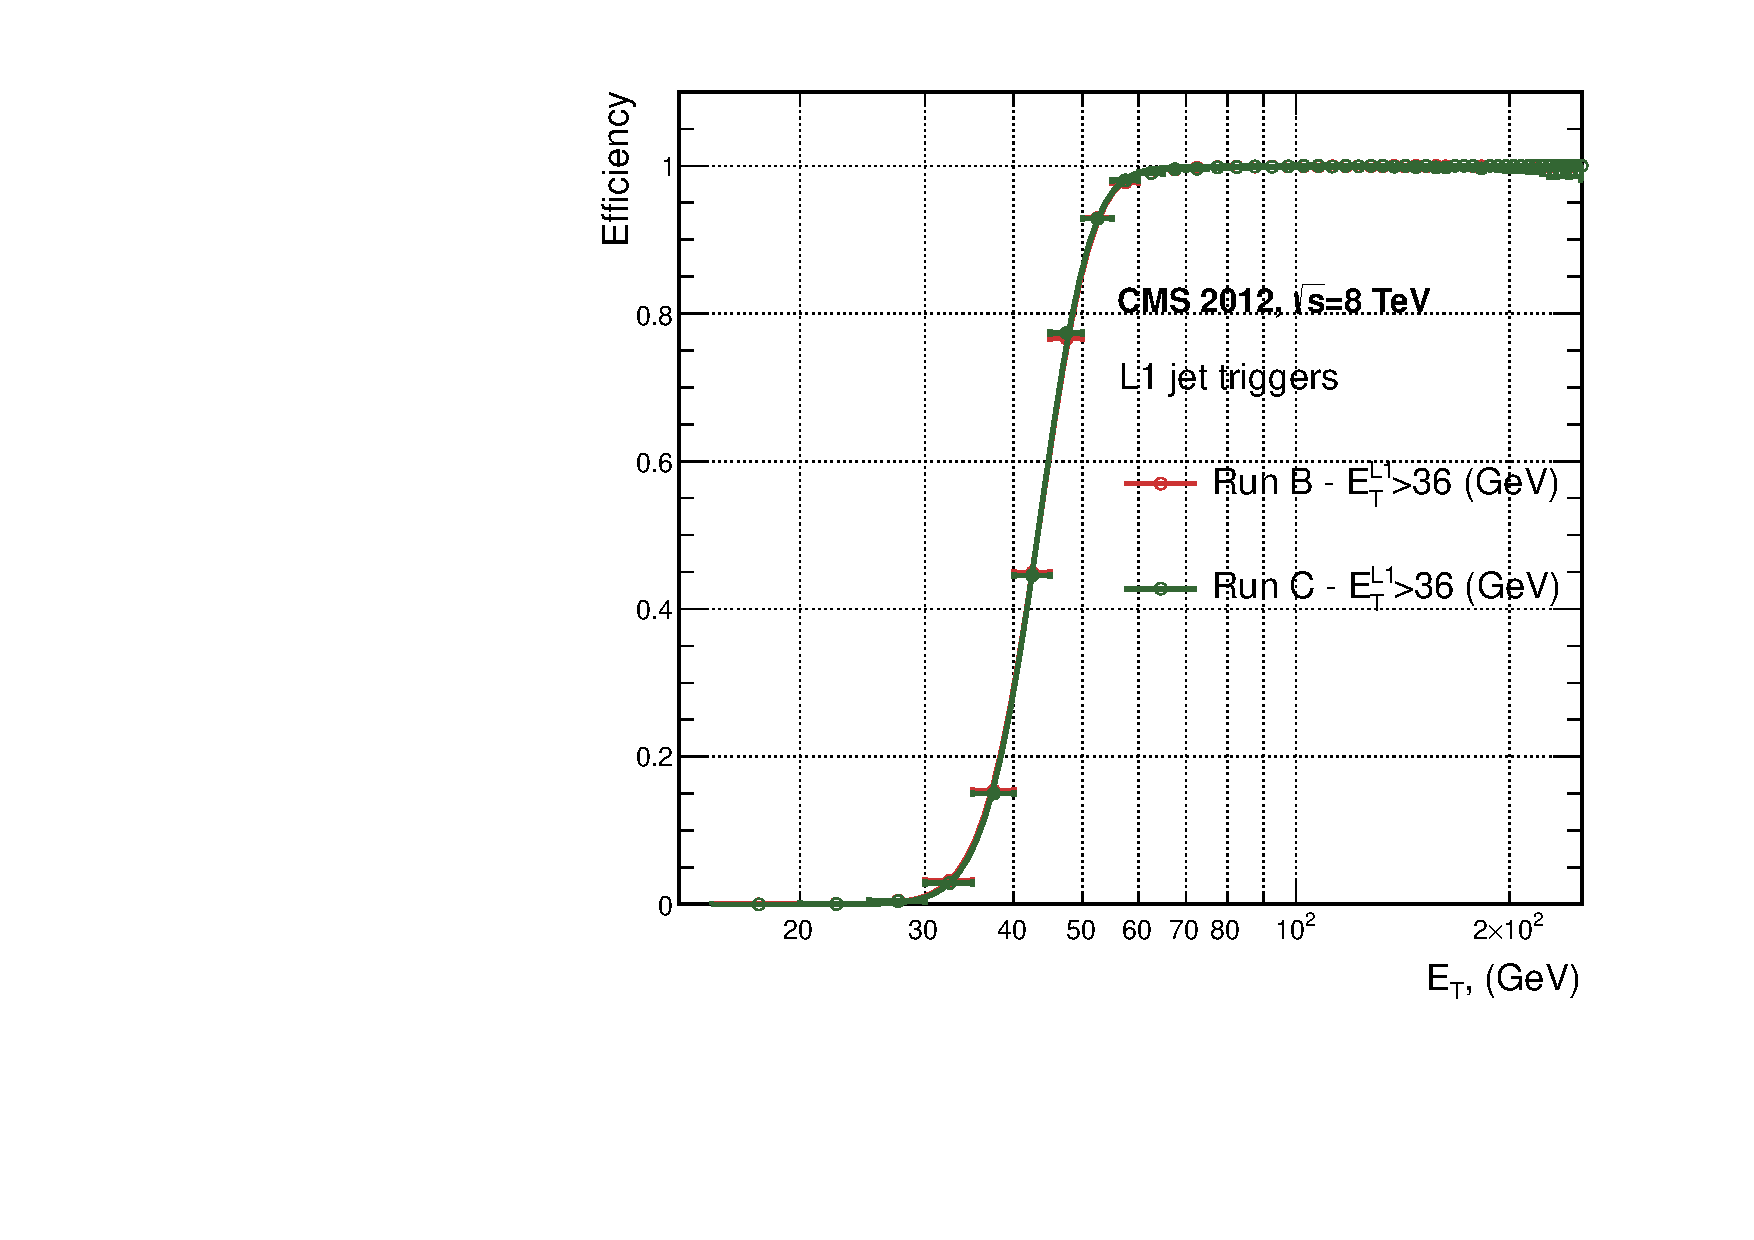
\includegraphics[width = 1.0\linewidth]{plots/jetseed_36.pdf}
\end{minipage}
\quad
\begin{minipage}[b]{0.48 \linewidth}
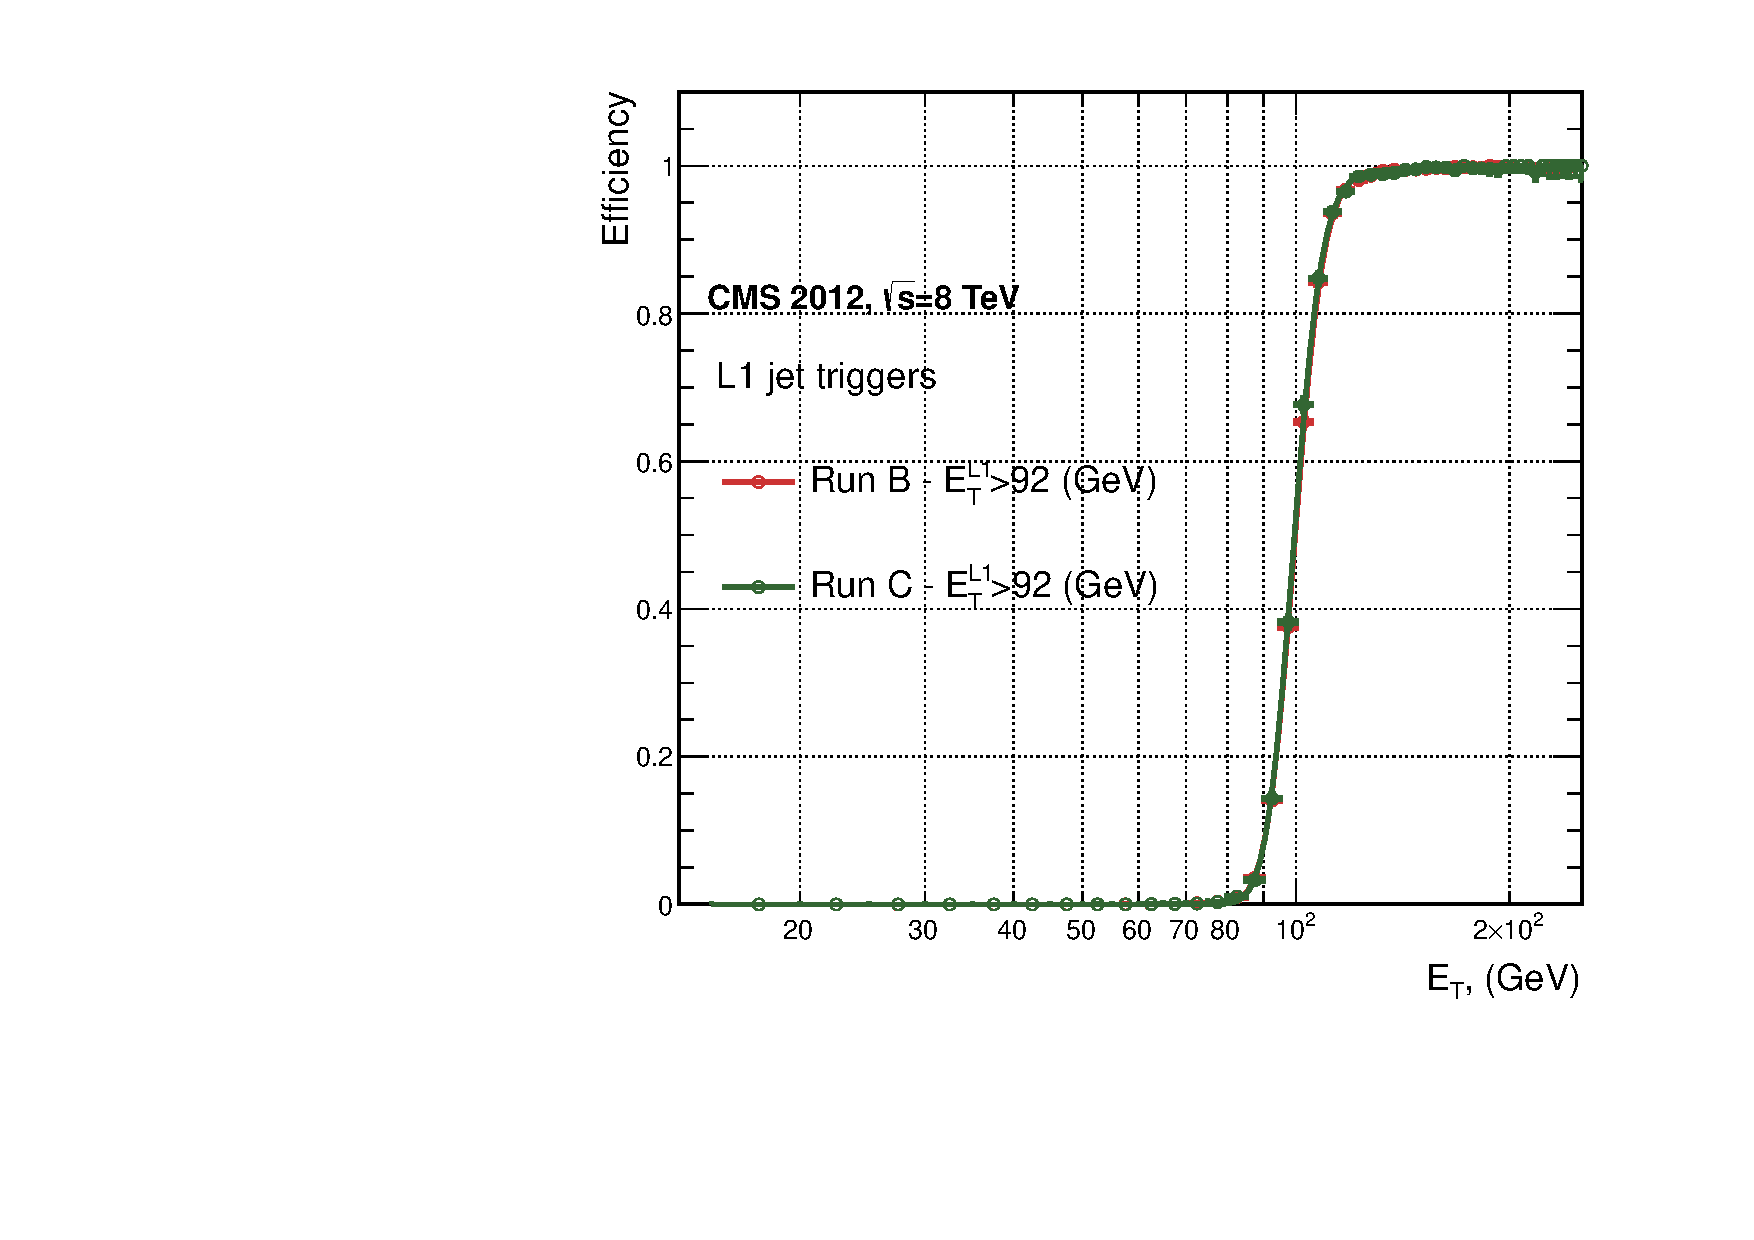
\includegraphics[width = 1.0\linewidth]{plots/jetseed_92.pdf}
\end{minipage}
\quad
\caption[L1 jet efficiency turn-on curves as a function of the offline CaloJet E$_{T}$ for the 2012 run period B and C.]{L1 jet efficiency turn-on curves as a function of the offline CaloJet E$_{T}$, measured for the \L1 SingleJet 36 and 92 trigger in 2012 run period B and C collected with an isolated single $\mu$ sample.}
\label{fig:l1jetseeds} 
\end{figure}

\begin{figure}[ht]
\centering
\begin{minipage}[b]{0.48 \linewidth}
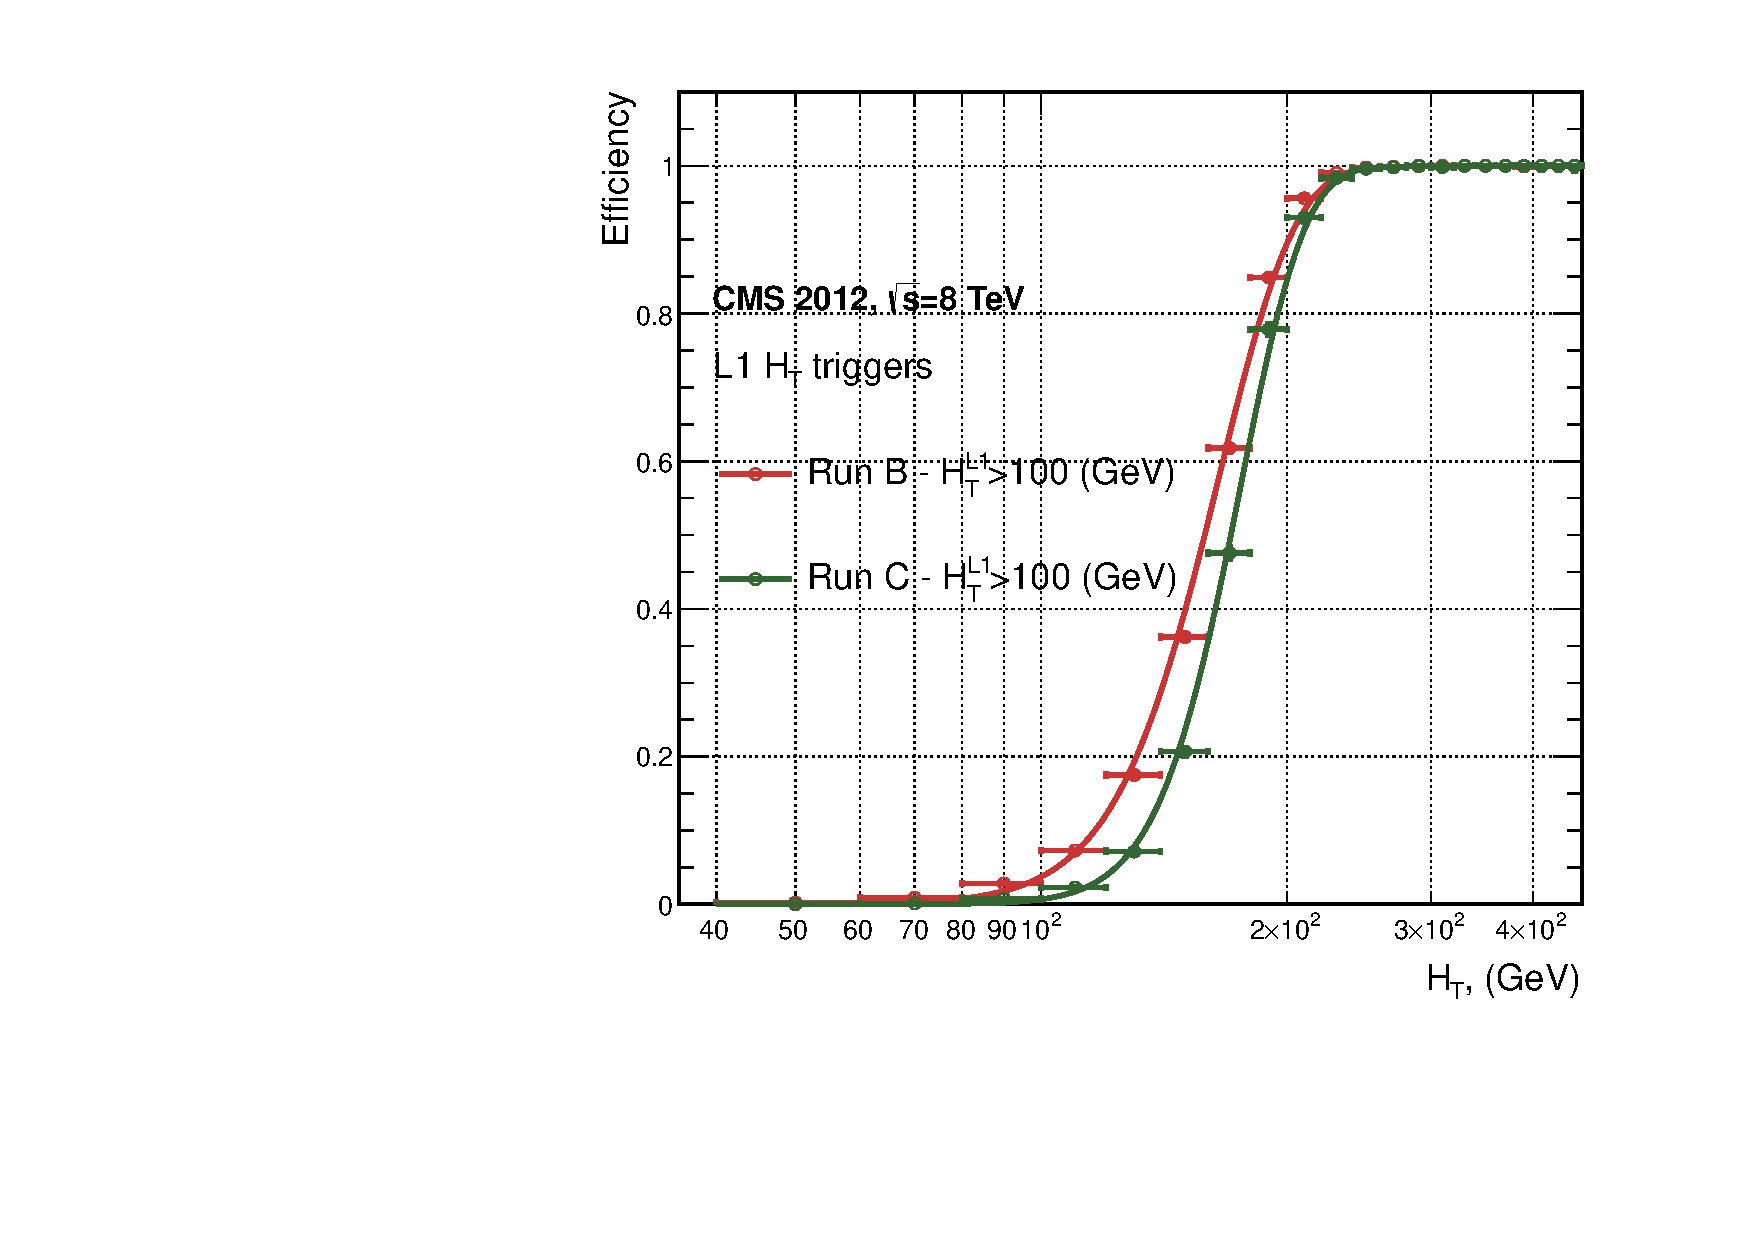
\includegraphics[width = 1.0\linewidth]{plots/jetseed_ht100.pdf}
\end{minipage}
\quad
\begin{minipage}[b]{0.48 \linewidth}
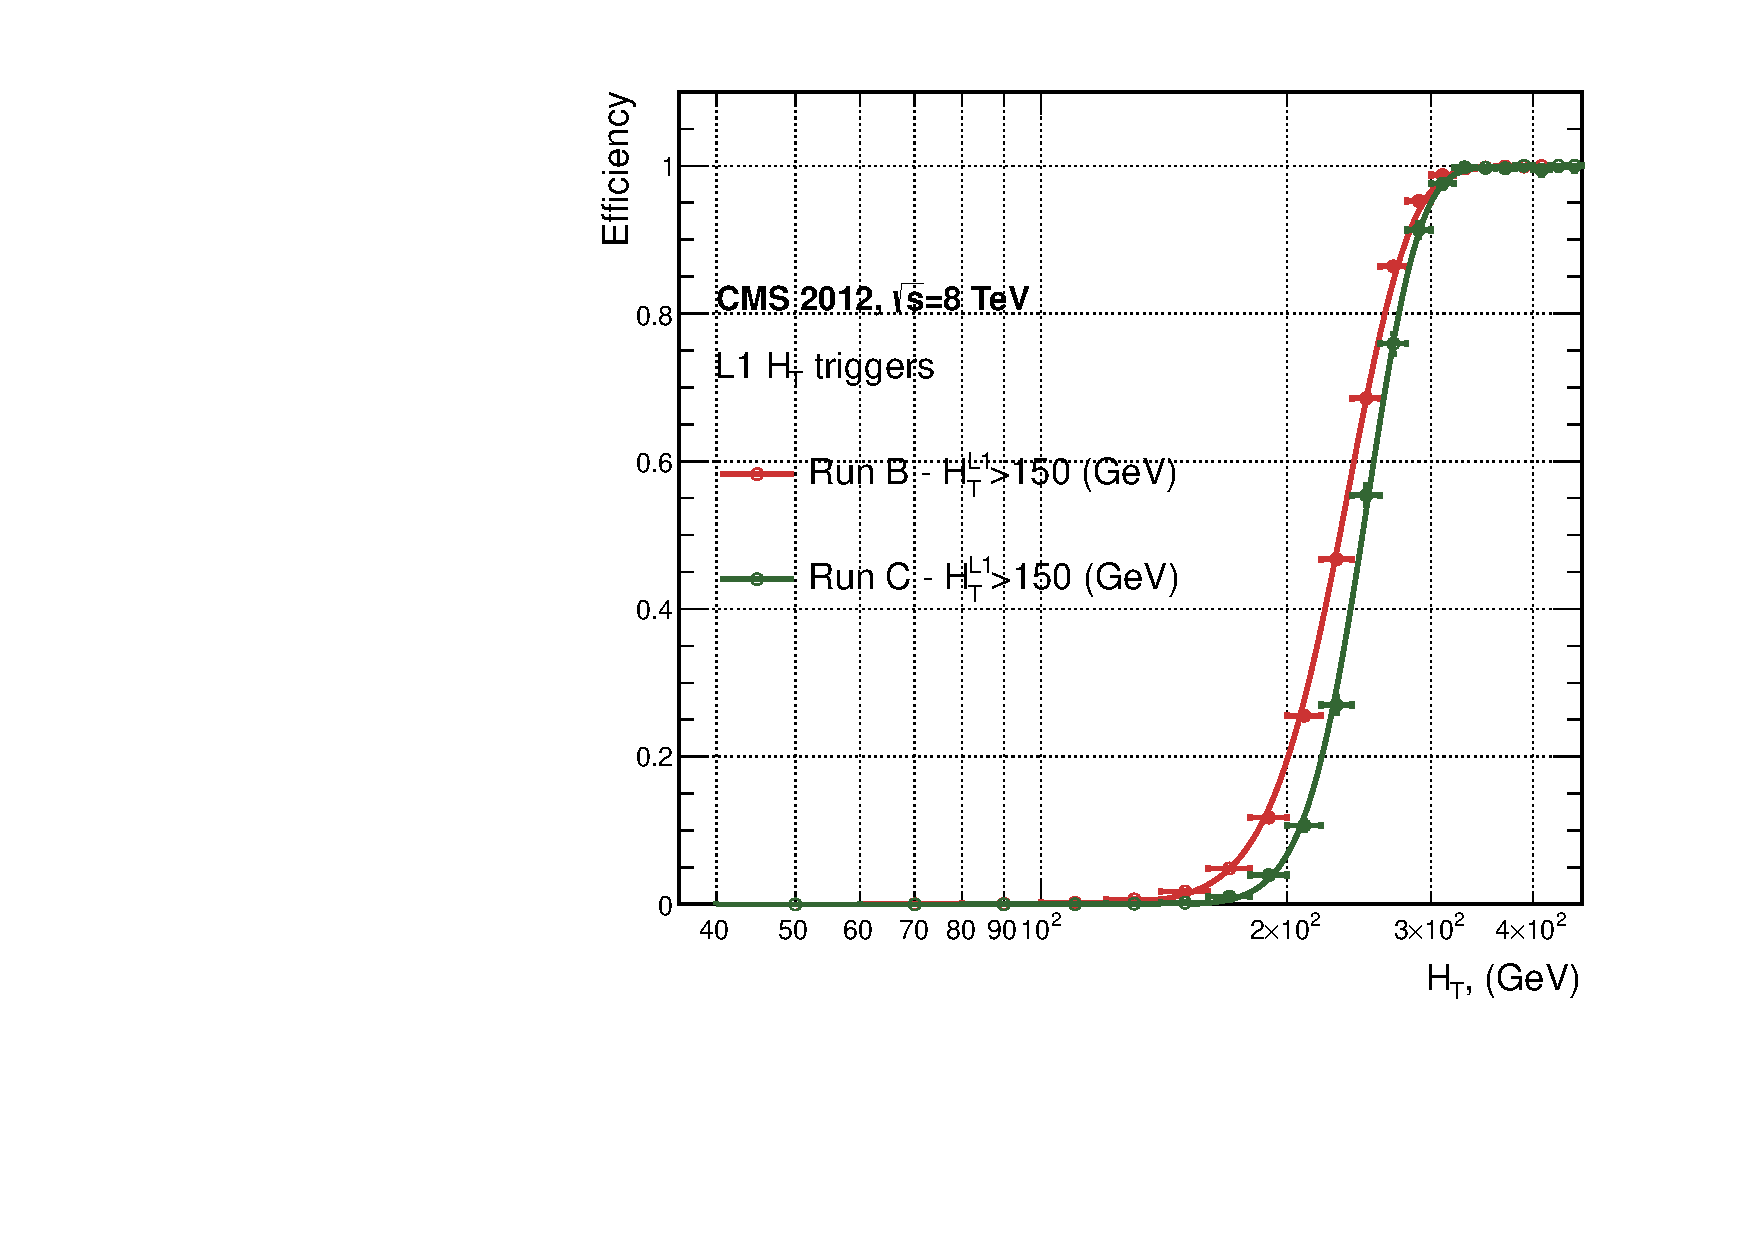
\includegraphics[width = 1.0\linewidth]{plots/jetseed_ht150.pdf}
\end{minipage}
\quad
\caption[\L1 $\theht$ efficiency turn-on curves as a function of the offline CaloJet $\theht$.]{\L1 $\theht$ efficiency turn-on curves as a function of the offline CaloJet $\theht$, measured for the \L1 $\theht$ 100 and 150 trigger during the run 2012 B and C, collected using an isolated single $\mu$ triggered sample.}
\label{fig:l1jetseedht} 
\end{figure}

It can be seen that the performance of the $E_{T} > 36,92$ single jet triggers are almost identical, with the jet seed having no measurable effect on these triggers as shown in Table \ref{tab:l1jetseedtable}. 

\begin{table}[h!]
\begin{center}
\footnotesize
\begin{tabular*}{0.75\textwidth}{@{\extracolsep{\fill}}c|cc|cc}
\hline
\multicolumn{1}{c}{}& \multicolumn{2}{c}{2012B} & \multicolumn{2}{c}{2012C} \\ 
\multicolumn{1}{c}{Trigger} & $\mu$ & \multicolumn{1}{c}{$\sigma$} & $\mu$ & $\sigma$ \\ \hline\hline
L1\_SingleJet36 & 40.29 $\pm$ 0.04& 5.34 $\pm$ 0.02 & 40.29 $\pm$ 0.11 & 5.21 $\pm$ 0.05 \\ 
L1\_SingleJet92 & 94.99 $\pm$ 0.09 & 5.93 $\pm$ 0.06 & 94.82 $\pm$ 0.29 & 5.74 $\pm$ 0.18 \\ 
\end{tabular*}
\end{center}
\caption[Results of a cumulative \ac{EMG} function fit to the turn-on curves for \L1 single jet triggers in the 2012 run period B and C.]{Results of a cumulative \ac{EMG} function fit to the turn-on curves for \L1 single jet triggers in the 2012 run period B and C, preselected on an isolated muon trigger. The turn-on point $\mu$ and resolution $\sigma$ of the L1 jet triggers are measured with respect to offline Calo Jets in run B (left) and run C (right). }
\label{tab:l1jetseedtable}

\end{table}


For the $\theht$ triggers, a large increase in trigger cross-section during high luminosity running without the jet seed threshold will occur. This is due to the low energy threshold required for a jet to be added to the \L1 $\theht$ sum, which is compiled from all clustered \L1 jets formed in the \ac{GCT}. The introduction of the jet seed threshold prevents the clustering of many of these soft low $\et$ jets, thus lowering the $\theht$ calculation at \L1. Different behaviours for the trigger turn-ons after the introduction of the jet seed threshold is therefore expected. The $\mu$ value is observed to shift towards higher $\theht$, whilst having a better resolution as a result of less pile-up jets being included in the \L1 $\theht$ sum. These measured values can be found within Table \ref{tab:l1jetseedtableHT}.


\begin{table}[h!]
\begin{center}
\footnotesize
\begin{tabular*}{0.75\textwidth}{@{\extracolsep{\fill}}c|cc|cc}
\hline
\multicolumn{1}{c}{}& \multicolumn{2}{c}{2012B} & \multicolumn{2}{c}{2012C} \\ 
\multicolumn{1}{c}{Trigger} & $\mu$ & \multicolumn{1}{c}{$\sigma$} & $\mu$ & $\sigma$ \\ \hline\hline
L1 HT-100 & 157.5 $\pm$ 0.08 & 32.9 $\pm$ 0.08 & 169.8 $\pm$ 0.08 & 28.7 $\pm$ 0.03 \\ 
L1 H1-150 & 230.9 $\pm$ 0.02 & 37.3 $\pm$ 0.01 & 246.4 $\pm$ 0.16 & 31.8 $\pm$ 0.05 \\ 
\end{tabular*}
\end{center}
\caption[Results of a cumulative \ac{EMG} function fit to the turn-on curves for $\theht$ in 2012 run period B and C.]{Results of a cumulative \ac{EMG} function fit to the turn-on curves for $\theht$ in run 2012 B and C, preselected on an isolated single $\mu$ trigger. The turn-on point $\mu$, resolution $\sigma$ of the \L1 $\theht$ triggers are measured with respect to offline $\theht$, formed from CaloJets with a $\et \geq 40$  in run period B (left) and C (right). }
\label{tab:l1jetseedtableHT}
\end{table}

Despite the slight increase in the $\mu$ value of the \theht triggers, the large benefit of this change upon the expected trigger cross section for the \L1 $\theht$ 150 trigger as a function of instantaneous luminosities can be clearly seen in Figure \ref{fig:l1rateplot}.

\begin{figure}[ht!]
\centering
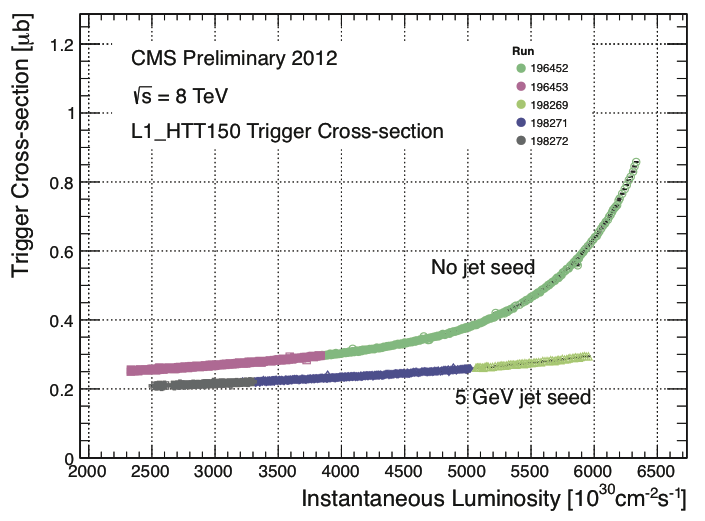
\includegraphics[scale=0.73]{plots/l1rateplot.pdf}
\caption[Trigger cross section for the \texttt{L1HTT150} trigger path. ]{Trigger cross section for the \texttt{L1HTT150} trigger path. Showing that a 5 \GeV jet seed threshold dramatically reduces the dependance of cross section on the instantaneous luminosity for \L1 $\theht$ triggers \cite{l1ratebrooke}.}  
\label{fig:l1rateplot}
\end{figure}  
\FloatBarrier

\subsection{Robustness of \L1 Jet Performance against Pile-up}
\label{subsec:l1jetpu}

The performance of the L1 single jet triggers is evaluated in different pile-up conditions to benchmark any dependence on pile-up. Three different pile-up bins of 0-10, 10-20 and $>$20 vertices are
defined, reflecting the low, medium and high pile-up running conditions at \ac{CMS} in 2012. This is benchmarked relative to \Calo and \PF jets for the run 2012 C period where the jet seed threshold is applied, with \L1 single jet thresholds of 16, 36 and 92 \GeV, shown in Figure \ref{fig:l1jet-calopf-pu}. The results of fitting an \ac{EMG} function to these efficiency turn-on curves are given in Table \ref{tab:l1jcaloputable} and Table \ref{tab:l1pfputable} for \Calo and \PF jets respectively.

\begin{figure}[ht]
\centering
\begin{minipage}[b]{0.48 \linewidth}
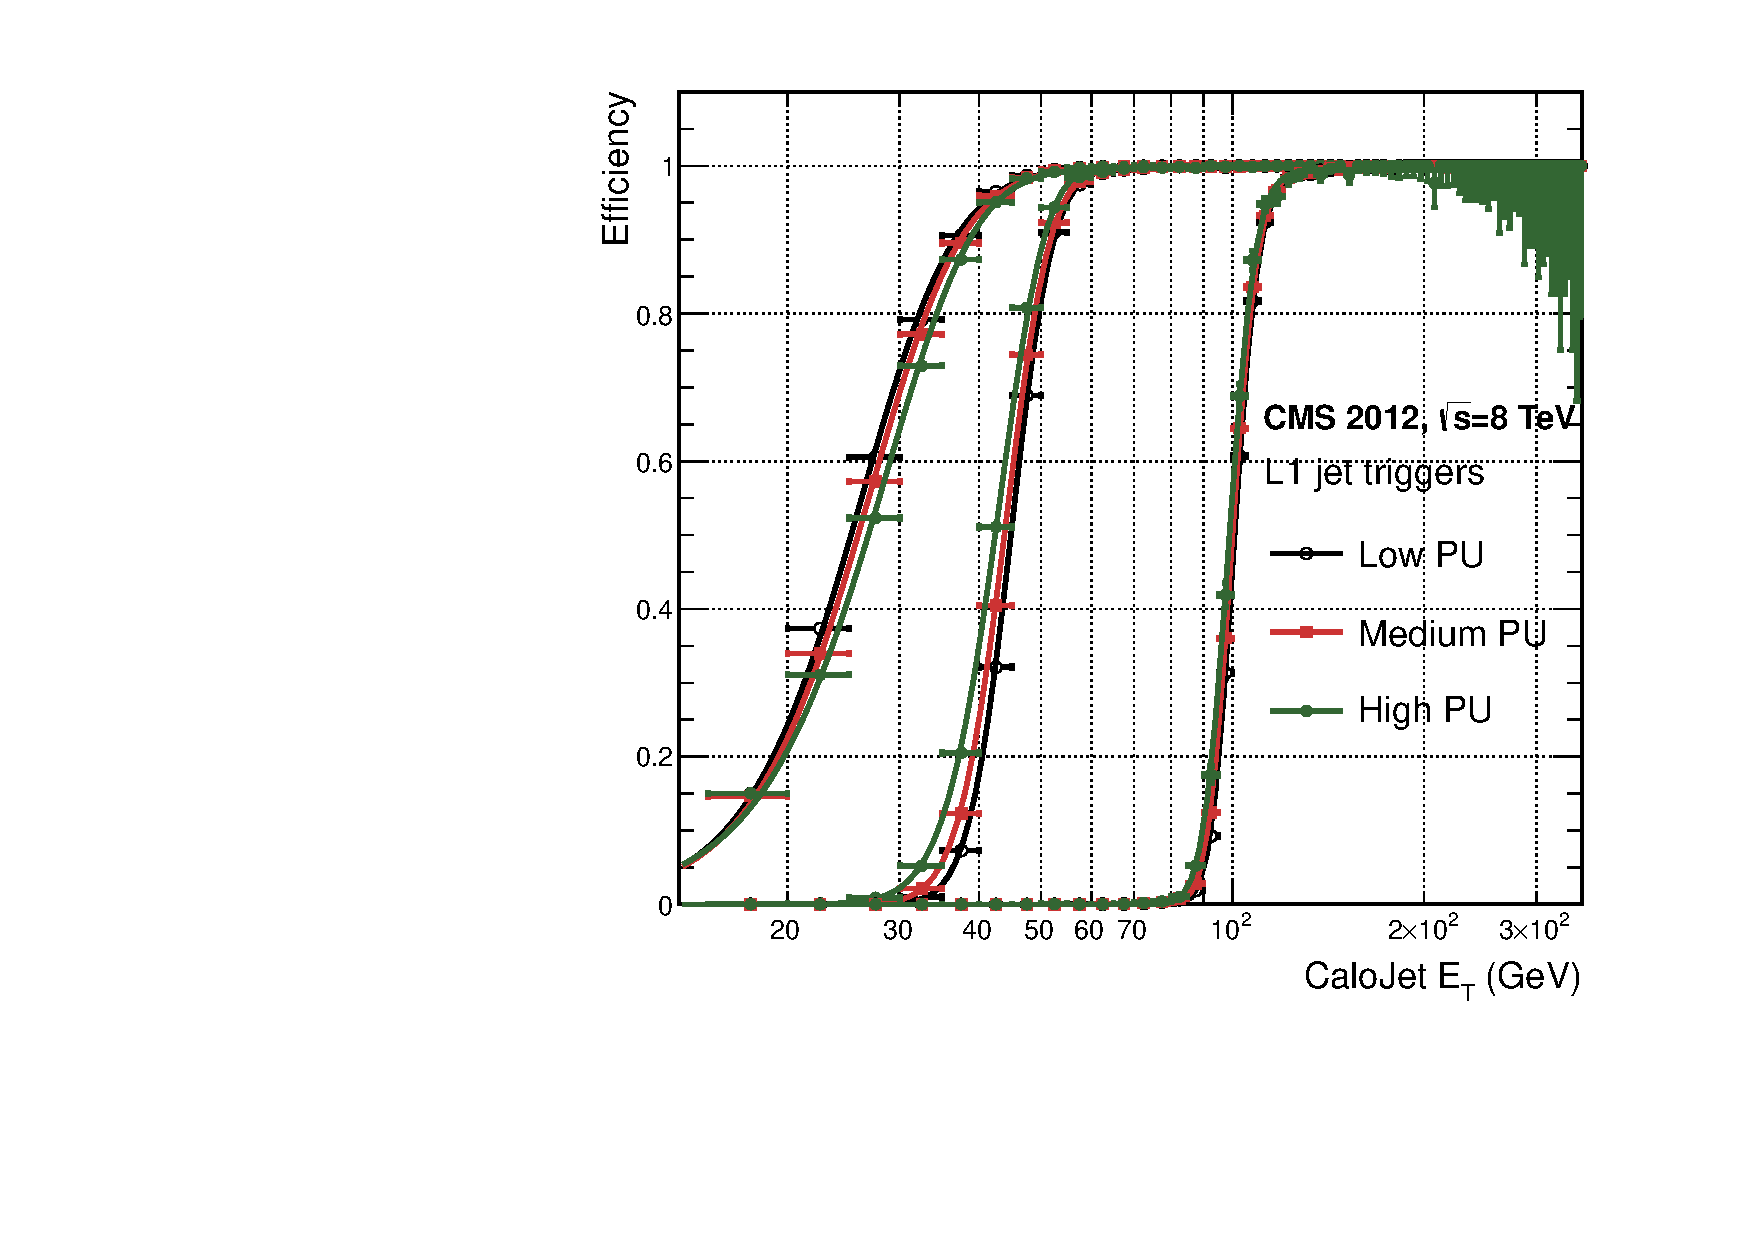
\includegraphics[width = 1.0\linewidth]{plots/jetpt_RunC_calopu.pdf}
\end{minipage}
\quad
\begin{minipage}[b]{0.48 \linewidth}
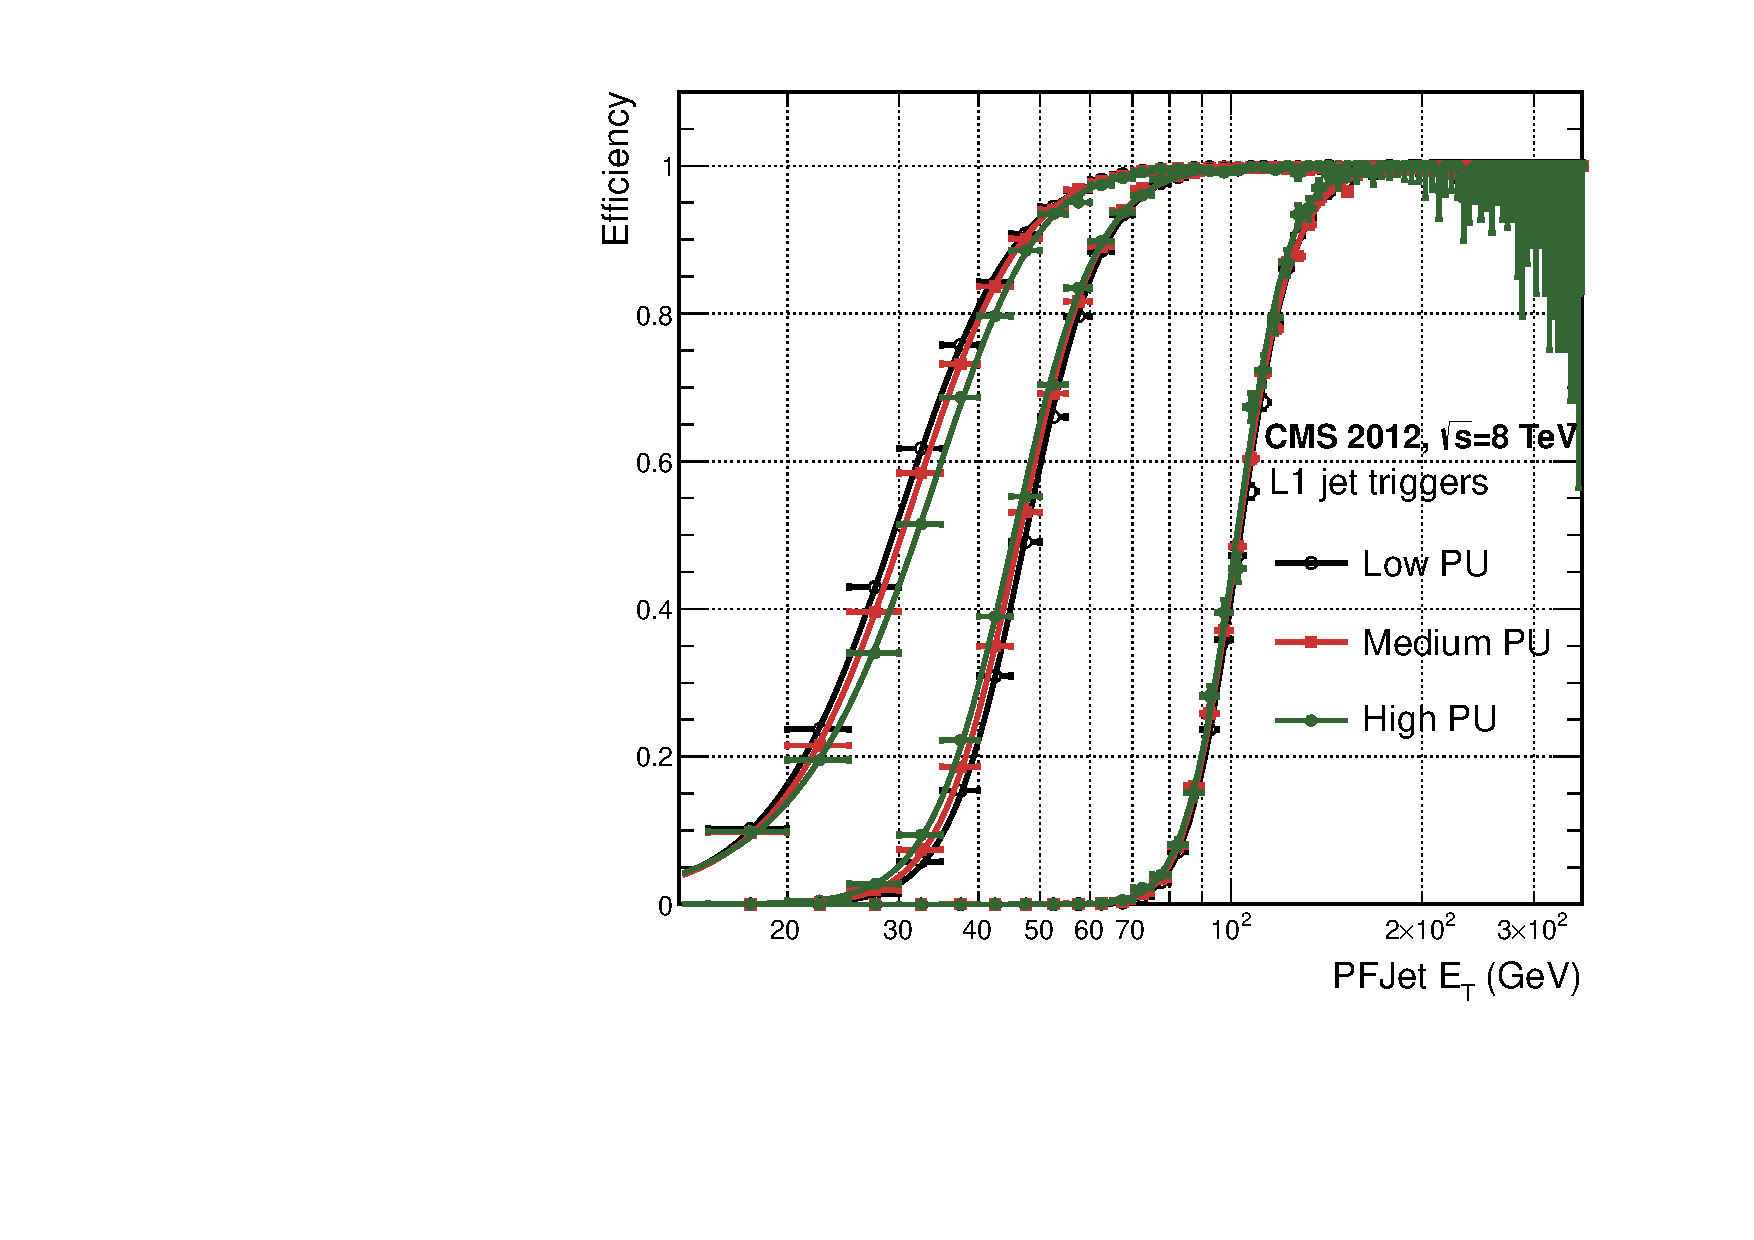
\includegraphics[width = 1.0\linewidth]{plots/jetpt_RunC_pfpu.pdf}
\end{minipage}
\quad
\caption[\L1 jet efficiency turn-on curves as a function of the leading offline $\et$ \Calo (left) and \PF (right) jet, for low, medium and high pile-up conditions.]{\L1 jet efficiency turn-on curves as a function of the leading offline $\et$\Calo (left) and \PF (right) jet, for low, medium and high pile-up conditions.}
\label{fig:l1jet-calopf-pu} 
\end{figure}



\begin{table}[ht]
%\begin{center}
\footnotesize
\begin{tabular*}{1.0\textwidth}{@{\extracolsep{\fill}}c|cc|cc|cc}
\hline
\multicolumn{1}{c}{Vertices} & \multicolumn{2}{c}{ 0-10 } & \multicolumn{2}{c}{11-20} & \multicolumn{2}{c}{$>$ 20}   \\ 
\multicolumn{1}{c}{} & $\mu$ & \multicolumn{1}{c}{$\sigma$} & $\mu$ & \multicolumn{1}{c}{$\sigma$} & $\mu$ & $\sigma$ \\ \hline\hline
L1\_SingleJet16 & 19.9 $\pm$ 0.1 & 6.1 $\pm$ 0.3  & 20.8 $\pm$ 0.1 & 6.5 $\pm$ 0.1 & 22.3 $\pm$ 0.2 & 7.5 $\pm$ 0.1\\ 
L1\_SingleJet36 & 41.8 $\pm$ 0.1 & 4.6 $\pm$ 0.1 & 40.9 $\pm$ 0.1 & 5.1 $\pm$ 0.1 & 40.6 $\pm$ 0.6 & 5.9 $\pm$ 0.2 \\ 
L1\_SingleJet92 & 95.9 $\pm$ 0.2 & 5.4 $\pm$ 0.1 & 95.2 $\pm$ 0.2 & 5.6 $\pm$ 0.1 & 94.5 $\pm$ 0.6 & 6.2 $\pm$ 0.3  \\ 
\end{tabular*}
%\end{center}
\caption[Results of a cumulative \ac{EMG} function fit to the efficiency turn-on curves for \L1 single jet triggers in the 2012 run period C, for low,medium and high pile-up conditions.]{Results of a cumulative \ac{EMG} function fit to the efficiency turn-on curves for \L1 single jet triggers in the 2012 run period C,  measured from isolated $\mu$ triggered data. The turn-on point, $\mu$, and resolution, $\sigma$, of the \L1 jet triggers are measured with respect to offline \Calo jets in low (left), medium (middle) and high (right) pile-up conditions. }
\label{tab:l1jcaloputable}
\end{table}

\begin{table}[ht]
%\begin{center}
\footnotesize
\begin{tabular*}{1.0\textwidth}{@{\extracolsep{\fill}}c|cc|cc|cc}
\hline
 \multicolumn{1}{c}{Vertices} & \multicolumn{2}{c}{ 0-10 } & \multicolumn{2}{c}{11-20} & \multicolumn{2}{c}{$>$ 20}   \\ 
 \multicolumn{1}{c}{} & $\mu$ & \multicolumn{1}{c}{$\sigma$} & $\mu$ & \multicolumn{1}{c}{$\sigma$} & $\mu$ & $\sigma$ \\ \hline\hline
L1\_SingleJet16 & 21.1 $\pm$ 0.1 & 7.16 $\pm$ 0.05 & 22.34 $\pm$ 0.1 & 7.9 $\pm$ 0.1 & 24.6 $\pm$ 0.2 & 9.5 $\pm$ 0.1 \\ 
L1\_SingleJet36 & 39.6 $\pm$ 0.1 & 7.4 $\pm$ 0.1 & 38.4 $\pm$ 0.1  & 7.4 $\pm$ 0.1 & 37.1 $\pm$ 0.2 & 7.5 $\pm$ 0.1 \\ 
L1\_SingleJet92 & 91.6 $\pm$ 0.3 & 11.3 $\pm$ 0.2 & 91.4 $\pm$ 0.3 & 11.2 $\pm$ 0.1 & 90.0 $\pm$ 0.9 & 12.1 $\pm$ 0.4  \\ 
\end{tabular*}
%\end{center}
\caption[Results of a cumulative \ac{EMG} function fit to the efficiency   turn-on curves for Level-1 single jet triggers in the 2012 run period C, for low,medium and high pile-up conditions.]{Results of a cumulative \ac{EMG} function fit to the efficiency   turn-on curves for Level-1 single jet triggers in the 2012 run period C, measured from isolated $\mu$ triggered data. The turn-on point, $\mu$, and resolution, $\sigma$, of the \L1 jet triggers are measured with respect to offline \PF jets in low (left), medium (middle) and high (right) pile-up conditions. }
\label{tab:l1pfputable}
\end{table}

No significant drop in efficiency is observed in the presence of a high number of primary vertices. The increase in hadronic activity in higher pile-up conditions, combined with the absence of pile-up subtraction for L1 jets, results in the expected observation of a decrease in the $\mu$ value of the efficiency turn-ons as a function of pile-up. Similarly, the resolution, $\sigma$, of the turn-ons are found to gradually grow due to the larger pile-up corrections being applied to the offline reconstructed jets.

These features are further emphasised when shown as a function of

\begin{equation}
\frac{(\text{L1 E}_{T} -  \text{Offline E}_{T})}{\text{Offline E}_{T}}
\label{eq:jetresolution}
\end{equation}

in bins of matched leading offline jet $\et$. The results of these individual fits categorised as a function of matched leading offline jet $\et$ can be found in Appendix (\ref{app:jetpuresolution}), where each of the distributions are fitted with an \ac{EMG} function as defined in Equation (\ref{eq:emg}).

The $\mu$, $\sigma$ and $\lambda$ values extracted for the low, medium and high pile-up conditions are shown for Calo and PF jets in Figure \ref{fig:jetptresultspu} and Figure \ref{fig:pfjetptresultspu} respectively. The central value of $\frac{(\text{L1 E}_{T} -  \text{Offline E}_{T})}{\text{Offline E}_{T}}$ is observed for all pile-up categories to increase as a function of jet $\et$, whilst the resolution is also observed to improve as a function of increasing offline jet $\et$. 

When comparisons are made between the individual pile-up scenarios, it can be seen that in the presence of higher pile-up , $\mu$ is seen to shift to larger values and a worsening resolution, $\sigma$, is observed. Both of these differences between the pile-up scenarios can once again be attributed to the increase in the number of soft pile-up jets in each category, combined with the absence of pile-up subtraction at \L1.

\begin{figure}[h!]
  \vspace{20pt}
	\centering
	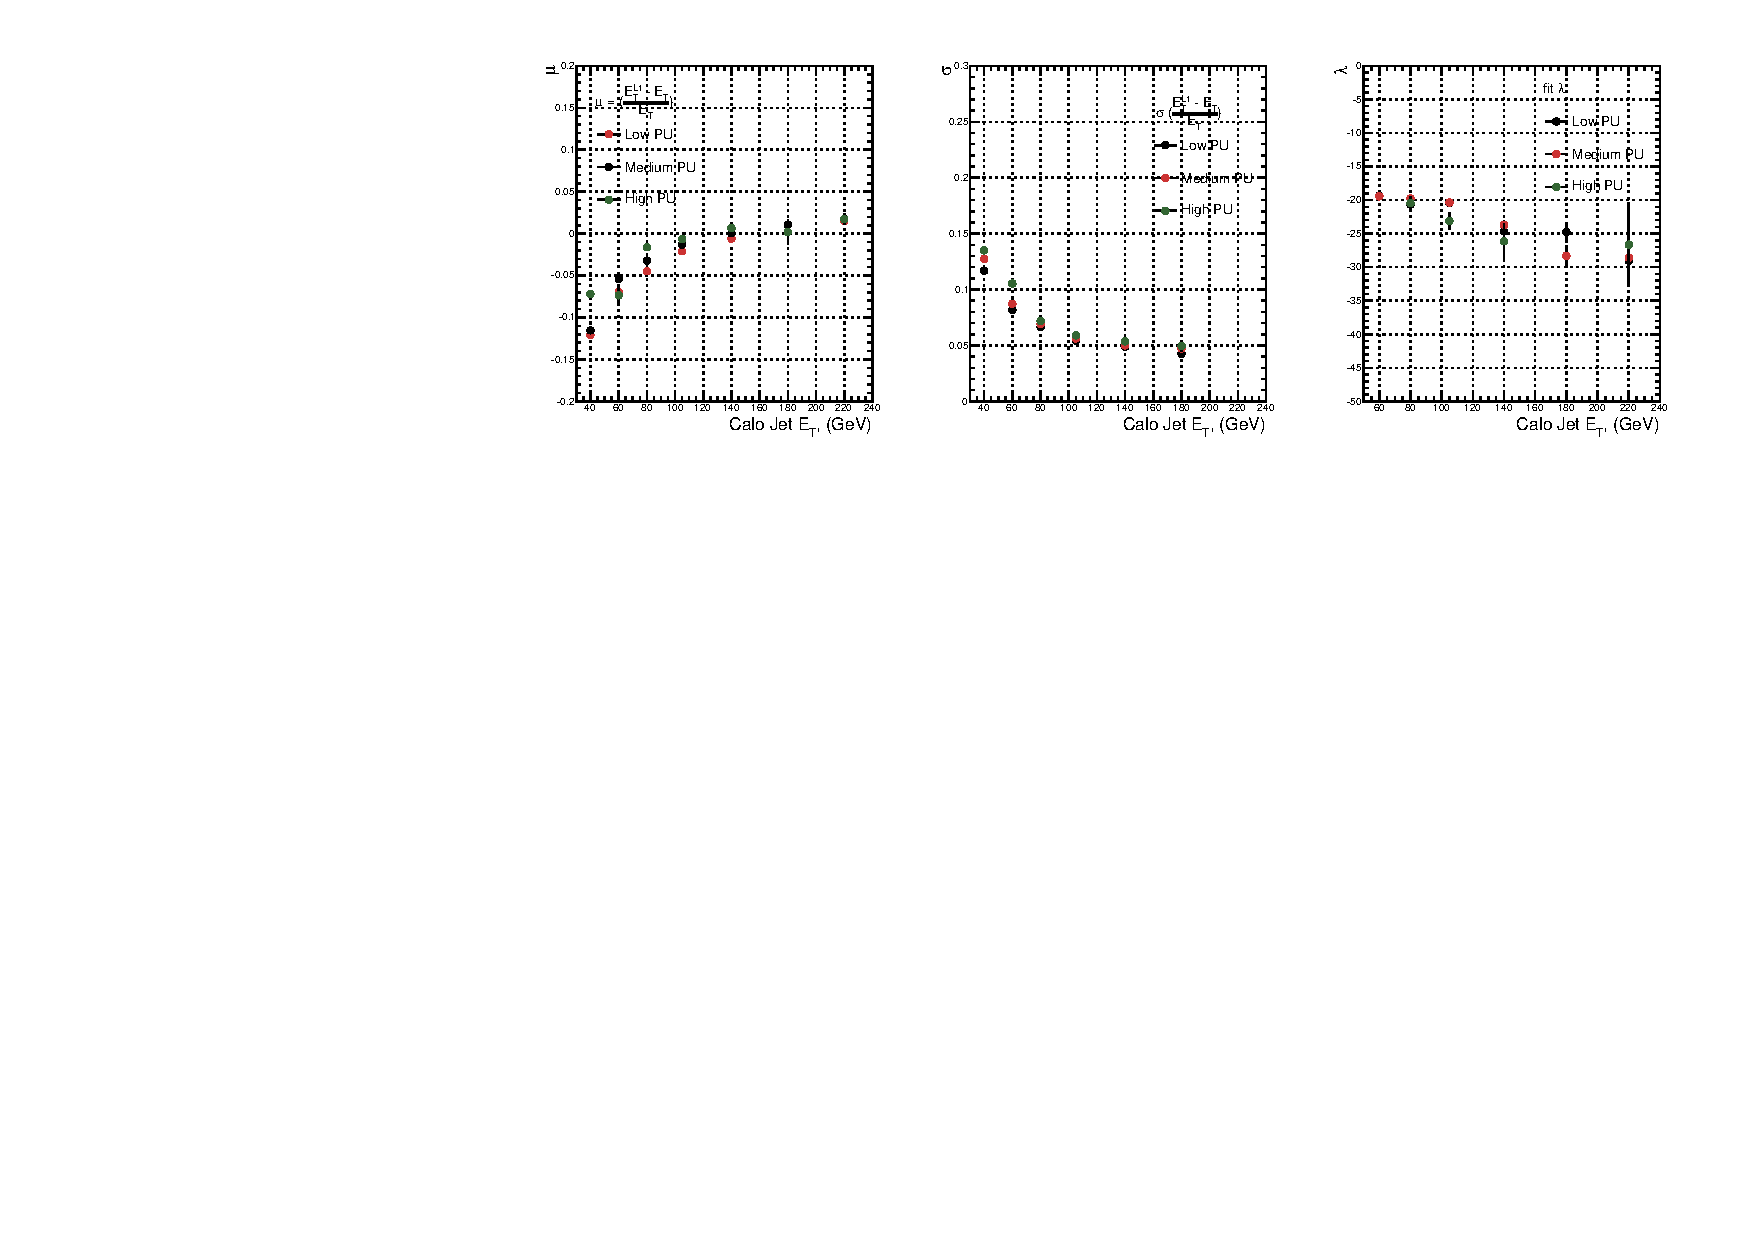
\includegraphics[width=1.0\textwidth]{plots/res_CaloJet_summary.pdf}
	\caption[Fit values from an \ac{EMG} function fitted to the resolution plots of leading Calo jet $\et$ measured as a function of  $\frac{(\text{L1 E}_{T} -  \text{Offline E}_{T})}{\text{Offline E}_{T}}$ for low, medium and high pile-up conditions. ]{Fit values from an \ac{EMG} function fitted to the resolution plots of leading Calo jet $\et$ measured as a function of  $\frac{(\text{L1 E}_{T} -  \text{Offline E}_{T})}{\text{Offline E}_{T}}$ for low, medium and high pile-up conditions. The plots show the mean $\mu$ (left), resolution $\sigma$ (middle) of the Gaussian as well as the decay term $\lambda$ (right) of the exponential.}
	\label{fig:jetptresultspu}
\end{figure}

\begin{figure}[h!]
  \vspace{20pt}
        \centering
        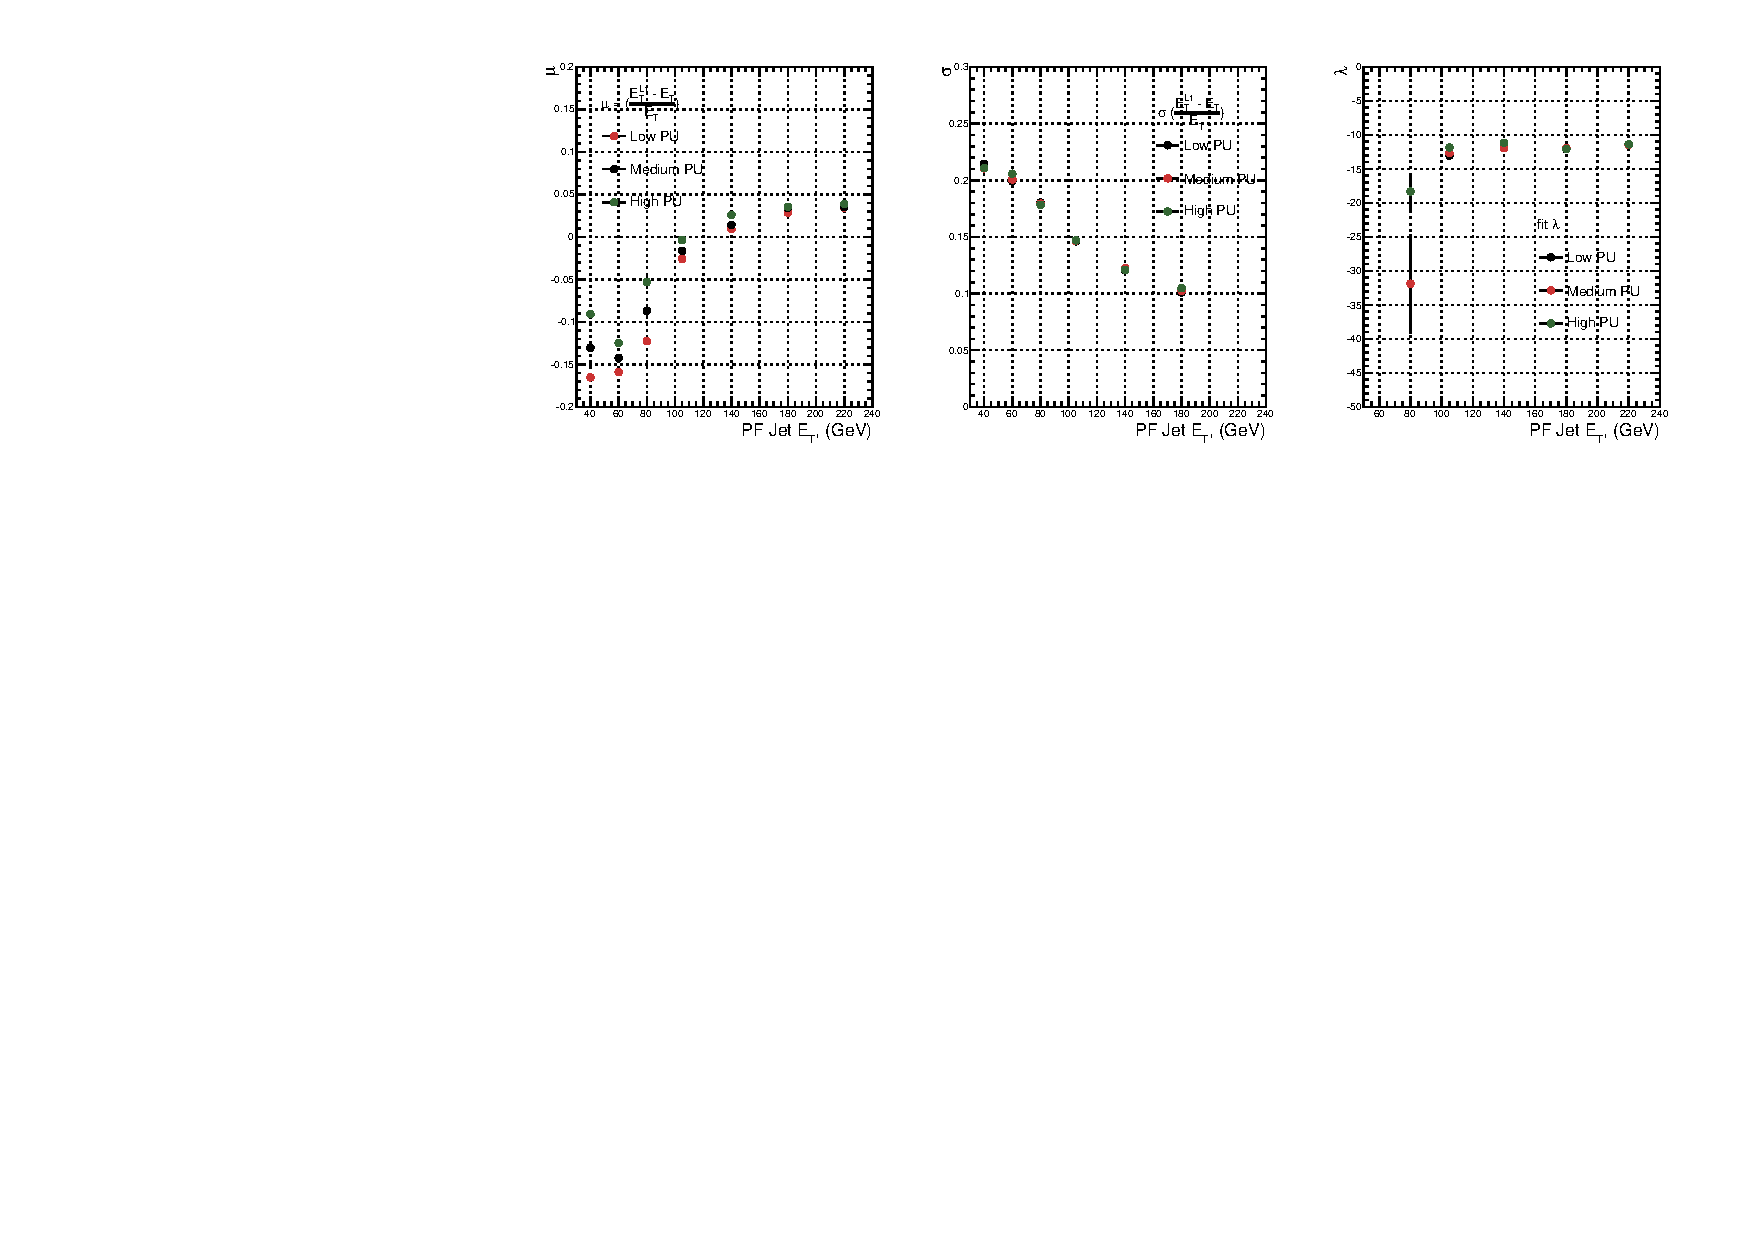
\includegraphics[width=1.0\textwidth]{plots/res_PFJet_summary.pdf}
        \caption[Fit values from an \ac{EMG} function fitted to the resolution plots of leading PF jet $\et$ measured as a function of  $\frac{(\text{L1 E}_{T} -  \text{Offline E}_{T})}{\text{Offline E}_{T}}$ for low, medium and high pile-up conditions.]{Fit values from an \ac{EMG} function fitted to the resolution plots of leading PF jet $\et$ measured as a function of  $\frac{(\text{L1 E}_{T} -  \text{Offline E}_{T})}{\text{Offline E}_{T}}$ for low and medium pile-up conditions. The plots show the mean $\mu$ (left), resolution $\sigma$ (middle) of the Gaussian, as well as the decay term $\lambda$ (right) of the exponential.}
        \label{fig:pfjetptresultspu}
\end{figure}

The resolution of other \L1 jet based energy sum quantities, $\mht$ and $\theht$ parameterised as in Equation (\ref{eq:jetresolution}), can be found in Appendix (\ref{app:jetenergysums}).

\subsection{Summary}
\label{subsec:l1summary}

The performance of the \CMS Level-1 Trigger has been studied and evaluated for jets and energy sum quantities using data collected during the 2012 \ac{lhc} 8 TeV run. These studies include the effect of the introduction of a 5 \GeV jet seed threshold into the jet clustering algorithm, the purpose of which is to mitigate the effects of pile-up on the rate of \L1 triggers, whilst not adversely affecting the efficiency of these triggers. No significant change in performance is observed with this change and good performance is observed for a range of \L1 quantities.

  \chapter{Searches for SUSY in Hadronic Final States at the LHC}
\label{chap:SUSYsearches}

In this chapter a model independent search for \ac{SUSY} in hadronic final states with $\met$ using the $\alphat$ variable and b-quark multiplicity is introduced and described in detail. The results presented are based on a data sample of pp collisions collected in 2012 at $\com =$8 \TeV, corresponding to an integrate luminosity of 11.7$\pm$0.5 fb$^{-1}$.

The kinematic variable $\alphat$ is motivated as a variable to provide strong rejections of QCD backgrounds, whilst maintaining sensitivity to possible a \ac{SUSY} signal within Section (\ref{sec:alphatintroduction}). The search and trigger strategy in addition to the event reconstruction and selection are outlined within Sections (\ref{subsec:searchstrategy}-\ref{subsec:eventselection}). 

The method in which the \ac{SM} background is estimated using an analytical technique to improve statistical precision at higher b-tag multiplicities is detailed within Section (\ref{subsec:backgroundestimation}), with a discussion on the impact of b-tagging and mis-tagging scale factors between data and MC on any background predictions. Finally a description of the formulation of appropriate systematic uncertainties applied to the background predictions to account for theoretical uncertainties and limitations in the simulation modelling of event kinematics and instrumental effects is covered in Section (\ref{subsec:sysuncertainties}).


In addition to the $\alphat$ search, a complimentary technique is discussed as a means to predict the distribution of 3 and 4 reconstructed b-quark jets in an event in Section (\ref{sec:templatemethod}). The recent discovery of the Higgs boson has made third-generation ``Natural \ac{SUSY}'' models attractive, given that light top and bottom squarks are a candidate to stabilise divergent loop corrections to the Higgs boson mass.

Using the $\alphat$ search as a base, a simple templated fit is employed to estimate the \ac{SM} background in higher b-tag multiplicities (3-4) from a region of a low number of reconstructed b-jets (0-2). The predictions using this technique are first tested in simulation before being compared to the \ac{SM} background predictions obtained from the $\alphat$ search.  

\section{The \alphat search}
\label{sec:alphatintroduction}

The experimental signature of \ac{SUSY} signal in the hadronic channel would manifest as a final state containing energetic jets and $\met$. The search focuses on topologies where new heavy supersymmetric, R-parity conserving particles are pair-produced in pp collisions. These particles decaying to a \ac{LSP} escape the detector undetected, leading to significant missing energy. 

A search within this channel is greatly complicated in a hadron collider environment, where the overwhelming background comes from inherently balanced multi-jet (``QCD'') events which are produced with an extremely large cross section. $\met$ can appear in such events with a substation mis-measurement of jet energy or missed objects due to detector miscalibration or noise effects. 

Additional \ac{SM} background contribution comes from \ac{EWK} processes with genuine $\met$�. 

\subsection{Search Strategy}
\label{subsec:searchstrategy}

\subsection{Trigger Strategy}
\label{subsec:triggerstrategy}

\subsection{Event Selection}
\label{subsec:eventselection}


\subsection{Background Estimation}
\label{subsec:backgroundestimation}


\subsection{Systematic Uncertainties on Transfer Factors}
\label{subsec:sysuncertainties}

\section{Searches for Natural SUSY with B-tag templates.}
\label{sec:templatemethod}

Btag Templates blah blah


  \chapter{Results And Interpretation}
\label{chap:SUSYresults}

Using the statistical framework outlined in the previous chapter, results are compared to a \ac{SM}-only hypothesis (Section (\ref{sec:smhypothesis})) and interpreted within various \ac{SMS} models (Section (\ref{sec:resultsms})). 

\section{Compatibility with the Standard Model Hypothesis}
\label{sec:smhypothesis}

The \ac{SM} background only hypothesis is tested by removing any signal contributions within the signal and control samples, and the likelihood function is maximised over all parameters using Rootfit \cite{2010acat.confE..57M} and MINUIT \cite{James:1975dr}. The results of the search consist of the observed yields in the hadronic signal sample, and the \mupjets, \dimupjets and \gpjets control samples. 

These observed yields along with the expectations and uncertainties given by the simultaneous fit for the hadronic signal region are given in Table \ref{tab:fitsdata}. The results obtained from the simultaneous fits, including that of the three control samples, are shown in Figure \ref{fig:result0blow}-\ref{fig:result4bhigh}, as summarised in Table \ref{tab:fitresults}. 

 \begin{table}[h!]
 \footnotesize
\begin{center}
\begin{tabular*}{0.55\textwidth}{@{\extracolsep{\fill}}cclc}
\hline
$n_{jet}$ & $n_{b}^{reco}$ & Control samples fitted & Figure  \\
\hline\hline
2-3 & 0 & \mupjets,\dimupjets,\gpjets & \ref{fig:result0blow} \\
2-3 & 1 & \mupjets,\dimupjets,\gpjets & \ref{fig:result1blow} \\
2-3 & 1 & \mupjets & \ref{fig:result2blow} \\
$\geq$4 & 0 & \mupjets,\dimupjets,\gpjets & \ref{fig:result0bhigh} \\
$\geq$4 & 1 & \mupjets,\dimupjets,\gpjets & \ref{fig:result1bhigh} \\
$\geq$4 & 2 & \mupjets & \ref{fig:result2bhigh} \\
$\geq$4 & 3 & \mupjets & \ref{fig:result3bhigh} \\
$\geq$4 & 4 & \mupjets & \ref{fig:result4bhigh} \\
\hline
\end{tabular*}
\end{center}
\caption[Summary of control samples used by each fit results, and the Figures in which they are displayed.]{Summary of control samples used by each fit results, and the Figures in which they are displayed.}\label{tab:fitresults}
\end{table}

 \begin{table}[h!]
 \footnotesize
\begin{center}
\begin{tabular*}{1.0\textwidth}{@{\extracolsep{\fill}}ccccccccccc}
\hline
& &&\multicolumn{8}{c}{\theht bin (\GeV)} \\
Cat & $n_{b}^{reco}$ & $n_{jet}$ &  275-325 & 325-375 & 375-475 & 474-575 & 575-675 & 675-775 & 775-875 & 875-$\infty$ \\
\hline\hline
SM & \multicolumn{1}{c}{\multirow{2}{*}{0}} & \multicolumn{1}{c}{\multirow{2}{*}{$\leq$ 3}} & 6235$^{+100}_{-67}$ & 2900$^{+60}_{-54}$ & $1955^{+34}_{-39}$& $558^{+14}_{-15}$ & $186^{+11}_{-10}$ & $51.3^{+3.4}_{-3.8}$ & $21.2^{+2.3}_{-2.2}$ & $16.1^{+1.7}_{-1.7}$ \\
Data &  &  & 6232 & 2904 & 1965 & 552 & 177 & 58 & 16 & 25 \\
\hline
SM & \multicolumn{1}{c}{\multirow{2}{*}{0}} & \multicolumn{1}{c}{\multirow{2}{*}{$\geq$ 4}} & 1010$^{+34}_{-24}$ & 447$^{+19}_{-16}$ & $390^{+19}_{-15}$& $250^{+12}_{-11}$ & $111^{+9}_{-7}$ & $53.3^{+4.3}_{-4.3}$ & $18.5^{+2.4}_{-2.4}$ & $19.4^{+2.5}_{-2.7}$ \\
Data &  &  & 1009 & 452 & 375 & 274 & 113 & 56 & 16 & 27 \\
\hline
SM & \multicolumn{1}{c}{\multirow{2}{*}{1}} & \multicolumn{1}{c}{\multirow{2}{*}{$\leq$ 3}} & 1162$^{+37}_{-29}$ & 481$^{+18}_{-19}$ & $341^{+15}_{-16}$& $86.7^{+4.2}_{-5.6}$ & $24.8^{+2.8}_{-2.7}$ & $7.2^{+1.1}_{-1.0}$ & $3.3^{+0.7}_{-0.7}$ & $2.1^{+0.5}_{-0.5}$ \\
Data &  &  & 1164 & 473 & 329 & 95 & 23 & 8 & 4 & 1 \\
\hline
SM & \multicolumn{1}{c}{\multirow{2}{*}{1}} & \multicolumn{1}{c}{\multirow{2}{*}{$\geq$ 4}} & 521$^{+25}_{-17}$ & 232$^{+15}_{-12}$ & $188^{+12}_{-11}$& $106^{+6}_{-6}$ & $42.1^{+4.1}_{-4.4}$ & $17.9^{+2.2}_{-2.0}$ & $9.8^{+1.5}_{-1.4}$ & $6.8^{+1.2}_{-1.1}$ \\
Data &  &  & 515 & 236 & 204 & 92 & 51 & 13 & 13 & 6 \\
\hline
SM & \multicolumn{1}{c}{\multirow{2}{*}{2}} & \multicolumn{1}{c}{\multirow{2}{*}{$\leq$ 3}} & 224$^{+15}_{-14}$ & 98.2$^{+8.4}_{-6.4}$ & $59.0^{+5.2}_{-6.0}$& $12.8^{+1.6}_{-1.6}$ & $3.0^{+0.9}_{-0.7}$ & $0.5^{+0.2}_{-0.2}$ & $0.1^{+0.1}_{-0.1}$ & $0.1^{+0.1}_{-0.1}$ \\
Data &  &  & 222 & 107 & 58 & 12 & 5 & 1 & 0 & 0 \\
\hline
SM & \multicolumn{1}{c}{\multirow{2}{*}{2}} & \multicolumn{1}{c}{\multirow{2}{*}{$\geq$ 4}} & 208$^{+17}_{-9}$ & 103$^{+9}_{-7}$ & $85.9^{+7.2}_{-6.9}$& $51.7^{+4.6}_{-4.7}$ & $19.9^{+3.4}_{-3.0}$ & $6.8^{+1.2}_{-1.3}$ & $1.7^{+0.7}_{-0.4}$ & $1.3^{+0.4}_{-0.3}$ \\
Data &  &  & 204 & 107 & 84 & 59 & 24 & 5 & 1 & 2 \\
\hline
SM & \multicolumn{1}{c}{\multirow{2}{*}{3}} & \multicolumn{1}{c}{\multirow{2}{*}{$\geq$ 4}} & 25.3$^{+5.0}_{-4.2}$ & 11.7$^{+1.7}_{-1.8}$ & $6.7^{+1.4}_{-1.2}$& $3.9^{+0.8}_{-0.8}$ & $2.3^{+0.6}_{-0.6}$ & $1.2^{+0.3}_{-0.4}$ & $0.3^{+0.2}_{-0.1}$ & $0.1^{+0.1}_{-0.1}$ \\
Data &  &  & 25 & 13 & 4 & 2 & 2 & 3 & 0 & 0 \\
\hline
SM & \multicolumn{1}{c}{\multirow{2}{*}{4}} & \multicolumn{1}{c}{\multirow{2}{*}{$\geq$ 4}} & 0.9$^{+0.4}_{-0.7}$ & 0.3$^{+0.2}_{-0.2}$ & \multicolumn{6}{c}{$0.6^{+0.3}_{-0.3}$} \\
Data &  &  & 1 & 0 & \multicolumn{6}{c}{2} \\
\hline
\end{tabular*}
\end{center}
\caption[Comparison of the measured yields in each \theht, $n_{jet}$ and $n_{b}^{reco}$ jet multiplicity bins for the hadronic sample with the \ac{SM} expectations and combined statistical and systematic uncertainties given by the simultaneous fit.]{Comparison of the measured yields in each \theht, $n_{jet}$ and $n_{b}^{reco}$ jet multiplicity bins for the hadronic sample with the \ac{SM} expectations and combined statistical and systematic uncertainties given by the simultaneous fit.}\label{tab:fitsdata}
\end{table}

The figures show a comparison between the observed yields and the \ac{SM} expectations across all \theht bins, and in all $n_{jet}$ and $n_{b}^{reco}$ multiplicity categories. In all categories the samples are well described by the \ac{SM} only hypothesis. In particular no significant excess is observed above \ac{SM} expectation within the hadronic signal region. 

Given the lack of an excess in data hinting at a possible supersymmetric signature within the data, interpretations are made on the production masses and cross section of  a range of \ac{SUSY} decay topologies within the following section.

\begin{figure}[ht]
\footnotesize
\centering
\begin{minipage}[b]{0.48 \linewidth}
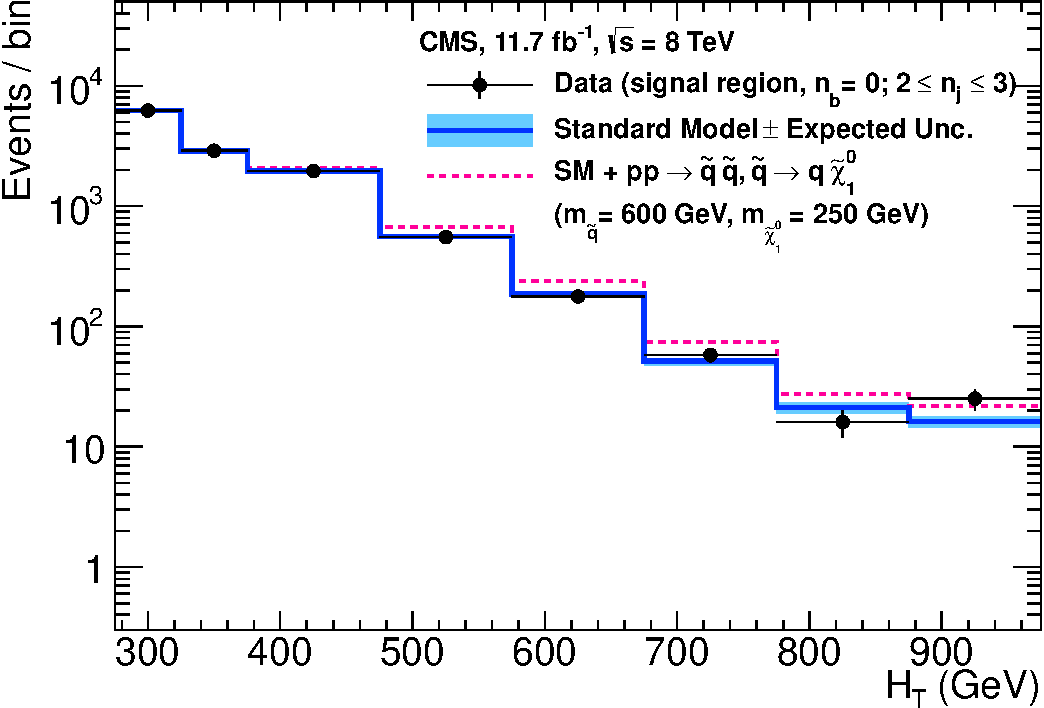
\includegraphics[width = 1.0\linewidth]{plots/hadronic_0b_le3j_logy.pdf}
\centering (a)  Hadronic sample, $2 \leq n_{jet} \leq 3$ and $n_{b}^{reco} = 0$ 
\end{minipage}
\quad
\begin{minipage}[b]{0.48\linewidth}
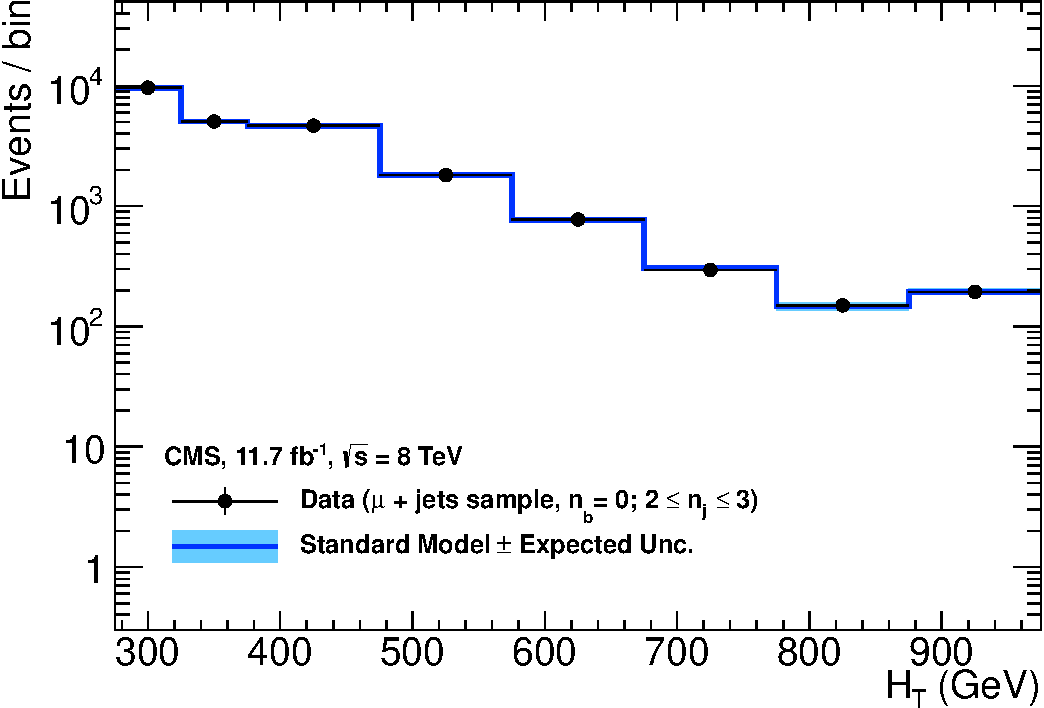
\includegraphics[width = 1.0\linewidth]{plots/muon_0b_le3j_logy.pdf}
\centering (b)  \mupjets sample, $2 \leq n_{jet} \leq 3$ and $n_{b}^{reco} = 0$  
\end{minipage} \\
\vspace{0.4cm}
\begin{minipage}[b]{0.48 \linewidth}
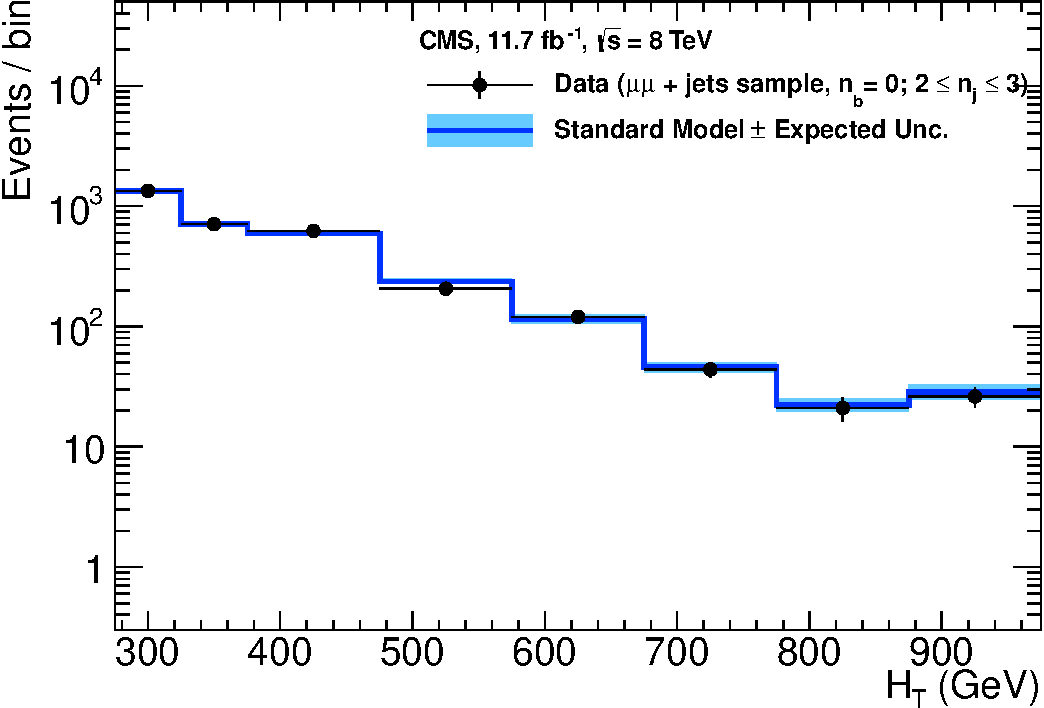
\includegraphics[width = 1.0\linewidth]{plots/mumu_0b_le3j_logy.pdf}
\centering (c$)$ \dimupjets sample, $2 \leq n_{jet} \leq 3$ and $n_{b}^{reco} = 0$ 
\end{minipage}
\quad
\begin{minipage}[b]{0.48\linewidth}
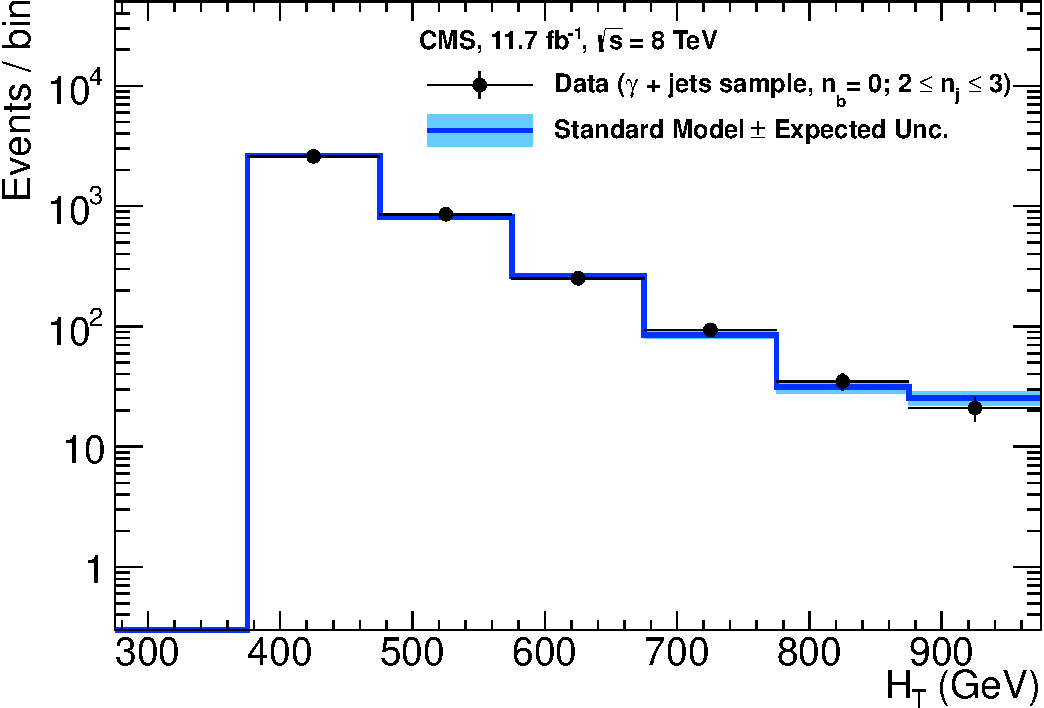
\includegraphics[width = 1.0\linewidth]{plots/photon_0b_le3j_logy.pdf}
\centering (d)  \gpjets sample, $2 \leq n_{jet} \leq 3$ and $n_{b}^{reco} = 0$ 
\end{minipage}
\caption[Comparison of the observed yields and \ac{SM} expectations given by the simultaneous fit in bins of \theht for the (a) hadronic, (b) \mupjets, (c$)$ \dimupjets and (d) \gpjets samples when requiring $n_{b}^{reco}$ = 0 and $n_{jet} \leq 3$.]{Comparison of the observed yields and \ac{SM} expectations given by the simultaneous fit in bins of \theht for the (a) hadronic, (b) \mupjets, (c$)$ \dimupjets and (d) \gpjets samples when requiring $n_{b}^{reco}$ = 0 and $n_{jet} \leq 3$. The observed event yields in data (black dots) and the expectations and their uncertainties for all SM processes (blue line with light blue bands) are shown. An example signal expectation (red solid line) for the $D1$ \ac{SMS} signal point from Table \ref{tab:sms_model_table} is superimposed on the \ac{SM} background expectation.}
\label{fig:result0blow}
\end{figure}

\begin{figure}[ht]
\footnotesize
\centering
\begin{minipage}[b]{0.48 \linewidth}
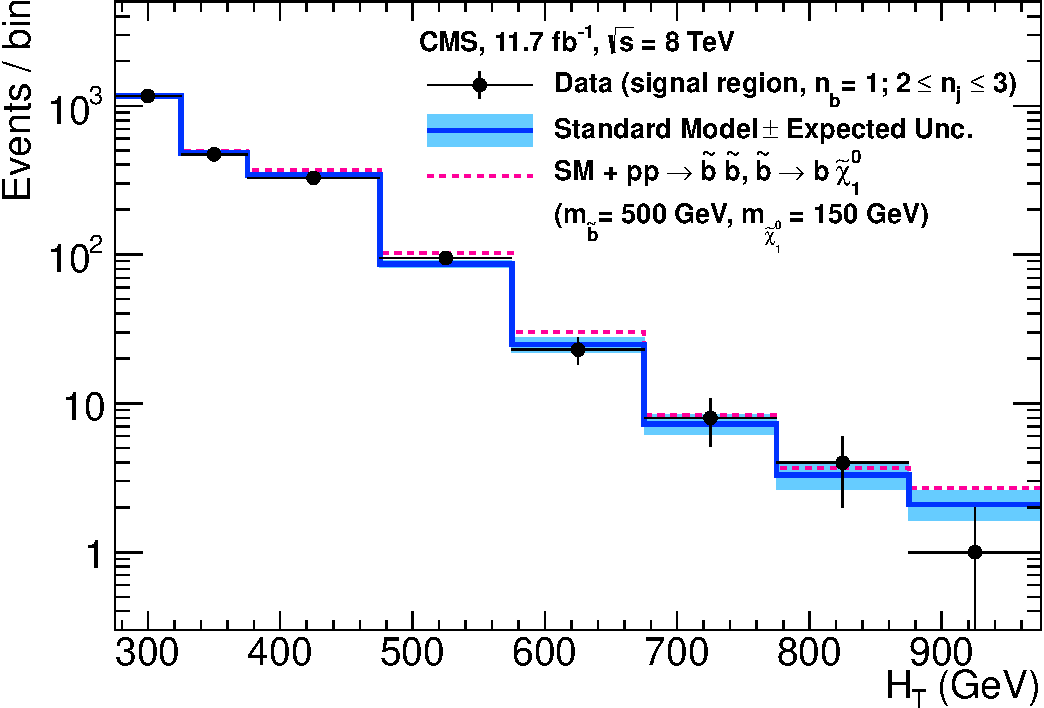
\includegraphics[width = 1.0\linewidth]{plots/hadronic_1b_le3j_logy.pdf}
\centering (a)  Hadronic sample, $2 \leq n_{jet} \leq 3$ and $n_{b}^{reco} = 1$ 
\end{minipage}
\quad
\begin{minipage}[b]{0.48\linewidth}
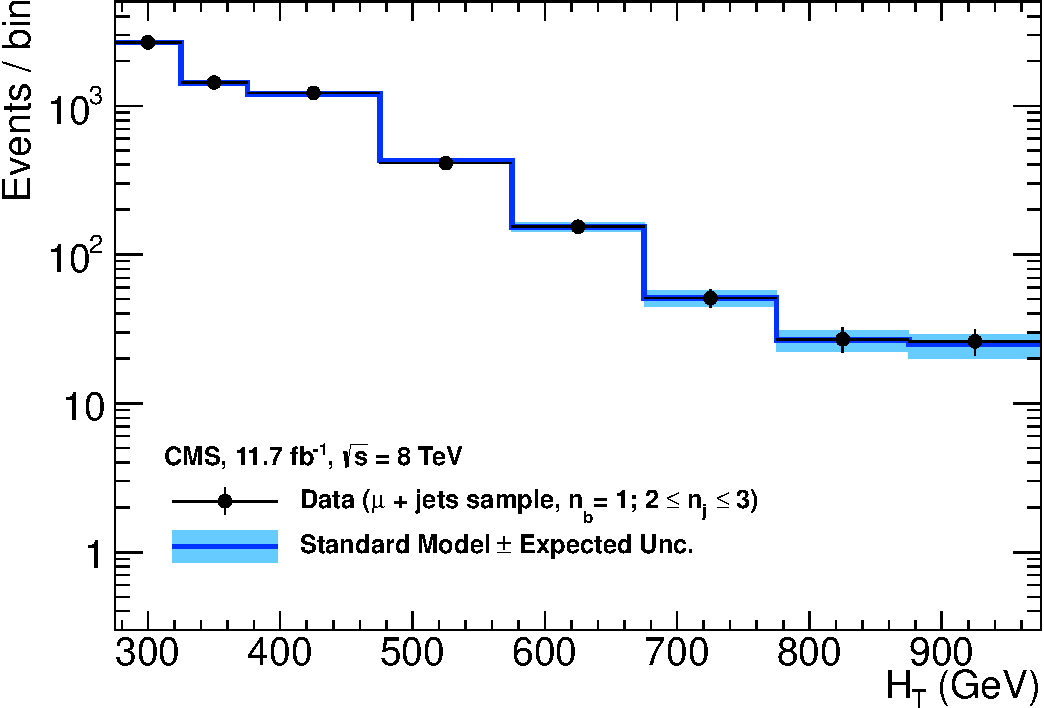
\includegraphics[width = 1.0\linewidth]{plots/muon_1b_le3j_logy.pdf}
\centering (b)  \mupjets sample, $2 \leq n_{jet} \leq 3$ and $n_{b}^{reco} = 1$  
\end{minipage} \\
\vspace{0.4cm}
\begin{minipage}[b]{0.48 \linewidth}
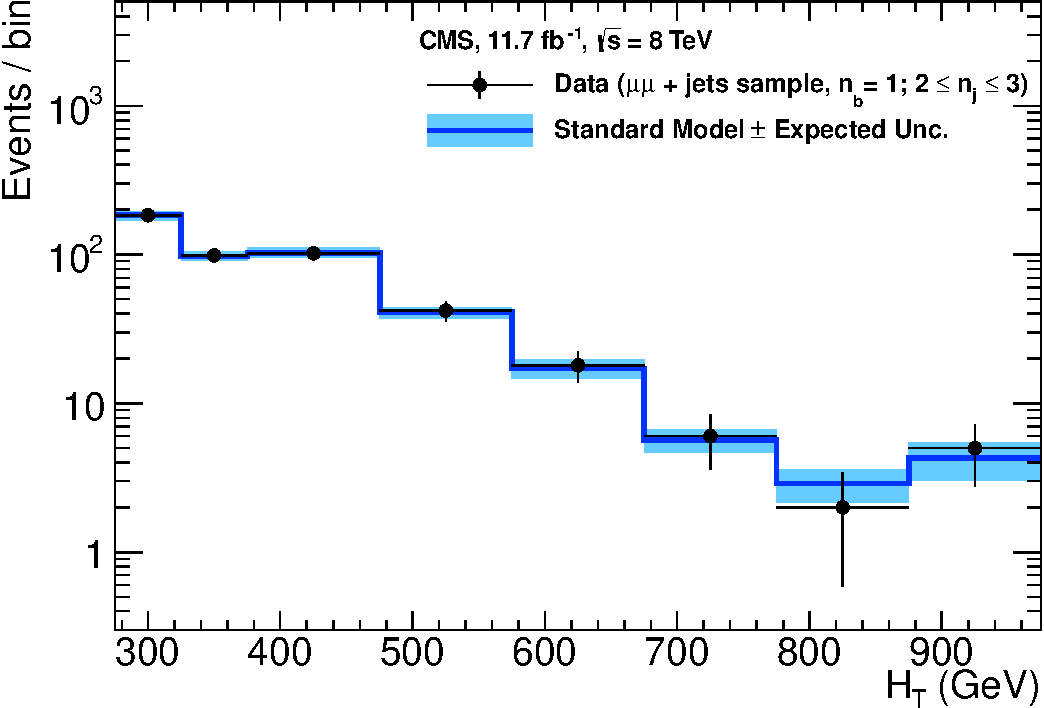
\includegraphics[width = 1.0\linewidth]{plots/mumu_1b_le3j_logy.pdf}
\centering (c$)$ \dimupjets sample, $2 \leq n_{jet} \leq 3$ and $n_{b}^{reco} = 1$ 
\end{minipage}
\quad
\begin{minipage}[b]{0.48\linewidth}
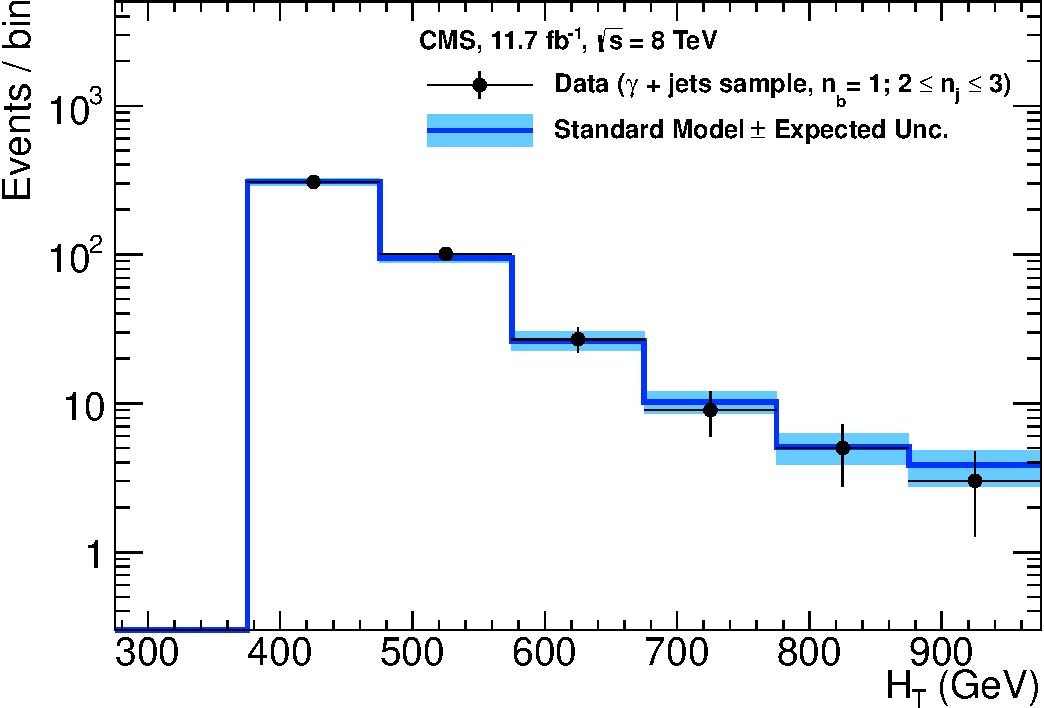
\includegraphics[width = 1.0\linewidth]{plots/photon_1b_le3j_logy.pdf}
\centering (d)  \gpjets sample, $2 \leq n_{jet} \leq 3$ and $n_{b}^{reco} = 1$ 
\end{minipage}
\caption[Comparison of the observed yields and \ac{SM} expectations given by the simultaneous fit in bins of \theht for the (a) hadronic, (b) \mupjets, (c$)$ \dimupjets and (d) \gpjets samples when requiring $n_{b}^{reco}$ = 1 and $n_{jet} \leq 3$.]{Comparison of the observed yields and \ac{SM} expectations given by the simultaneous fit in bins of \theht for the (a) hadronic, (b) \mupjets, (c$)$ \dimupjets and (d) \gpjets samples when requiring $n_{b}^{reco}$ = 1 and $n_{jet} \leq 3$. The observed event yields in data (black dots) and the expectations and their uncertainties for all SM processes (blue line with light blue bands) are shown. An example signal expectation (red solid line) for the $D2$ \ac{SMS} signal point from Table \ref{tab:sms_model_table} is superimposed on the \ac{SM} background expectation.}
\label{fig:result1blow}
\end{figure}

\begin{figure}[ht]
\footnotesize
\centering
\begin{minipage}[b]{0.48 \linewidth}
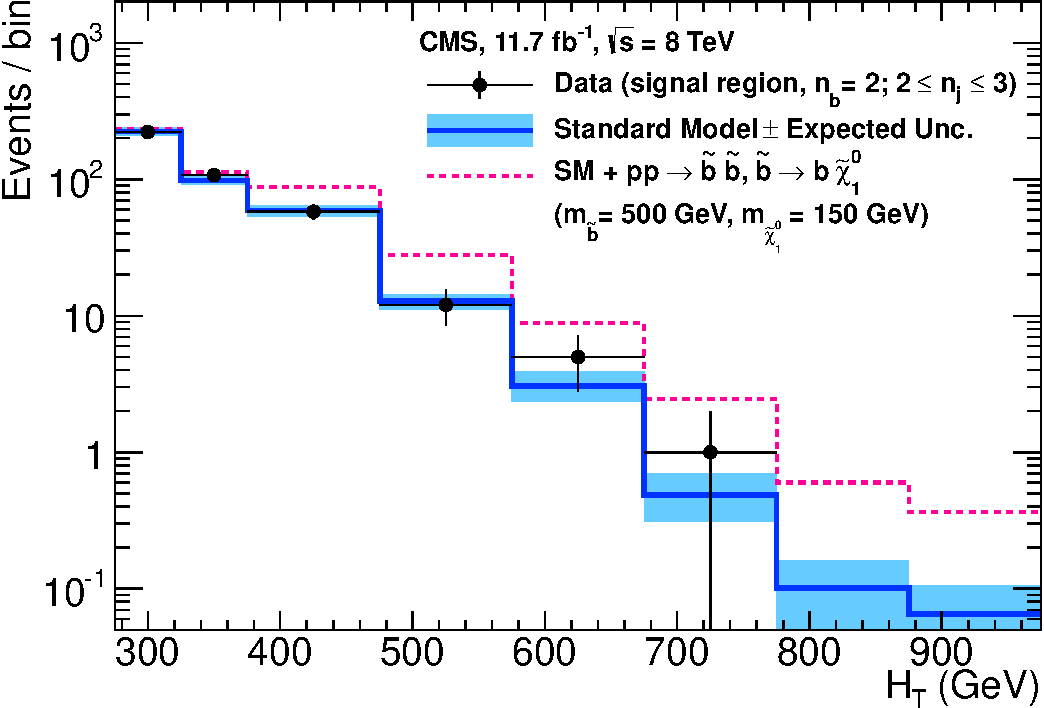
\includegraphics[width = 1.0\linewidth]{plots/hadronic_2b_le3j_logy.pdf}
\centering (a)  Hadronic sample, $2 \leq n_{jet} \leq 3$ and $n_{b}^{reco} = 2$ 
\end{minipage}
\quad
\begin{minipage}[b]{0.48\linewidth}
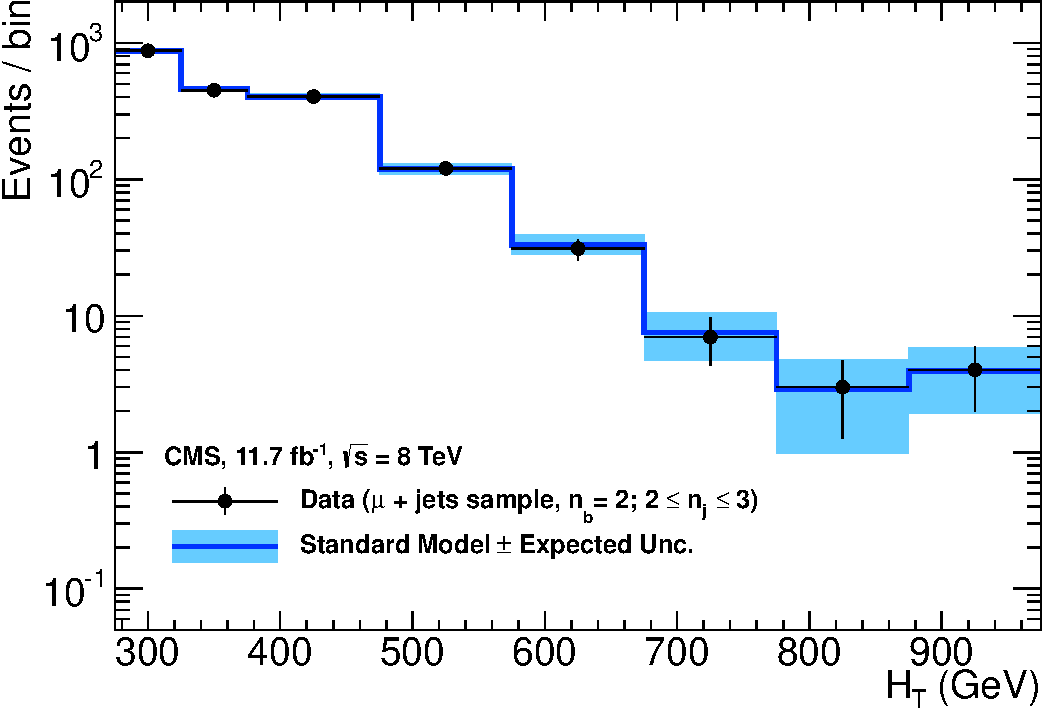
\includegraphics[width = 1.0\linewidth]{plots/muon_2b_le3j_logy.pdf}
\centering (b)  \mupjets sample, $2 \leq n_{jet} \leq 3$ and $n_{b}^{reco} = 2$  
\end{minipage} \\
\caption[Comparison of the observed yields and \ac{SM} expectations given by the simultaneous fit in bins of \theht for the (a) hadronic, (b) \mupjets, (c$)$ \dimupjets and (d) \gpjets samples when requiring $n_{b}^{reco}$ = 2 and $n_{jet} \leq 3$.]{Comparison of the observed yields and \ac{SM} expectations given by the simultaneous fit in bins of \theht for the (a) hadronic, (b) \mupjets, (c$)$ \dimupjets and (d) \gpjets samples when requiring $n_{b}^{reco}$ = 2 and $n_{jet} \leq 3$. The observed event yields in data (black dots) and the expectations and their uncertainties for all SM processes (blue line with light blue bands) are shown. An example signal expectation (red solid line) for the $D2$ \ac{SMS} signal point from Table \ref{tab:sms_model_table} is superimposed on the \ac{SM} background expectation.}
\label{fig:result2blow}
\end{figure}

\begin{figure}[ht]
\footnotesize
\centering
\begin{minipage}[b]{0.48 \linewidth}
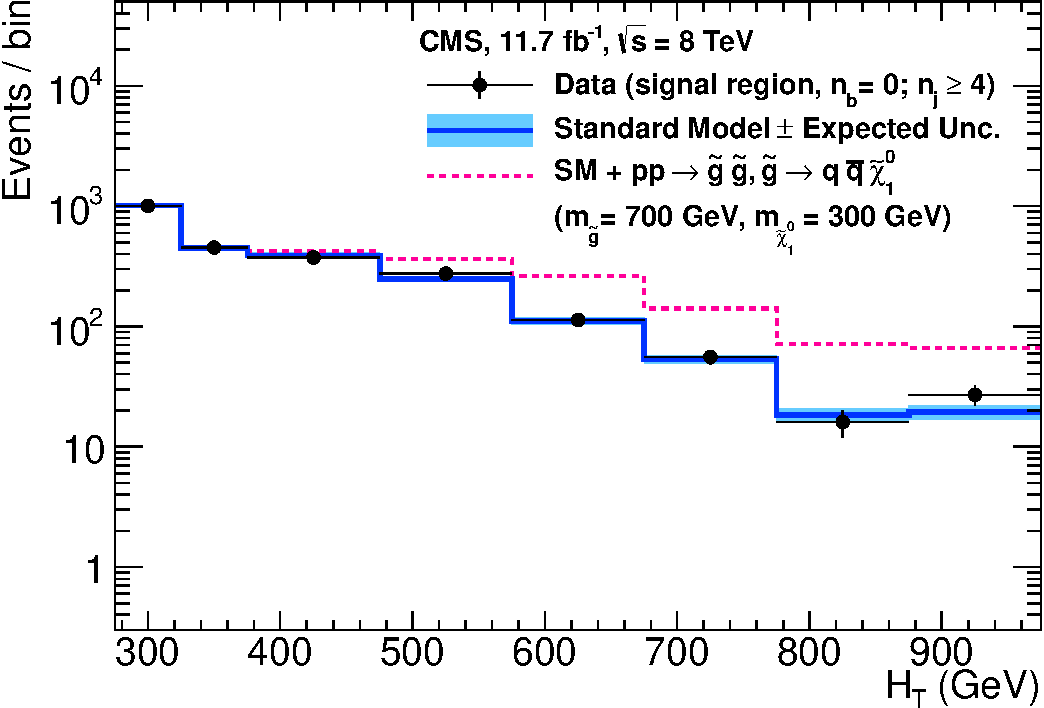
\includegraphics[width = 1.0\linewidth]{plots/hadronic_0b_ge4j_logy.pdf}
\centering (a)  Hadronic sample, $n_{jet} \geq 4$ and $n_{b}^{reco} = 0$ 
\end{minipage}
\quad
\begin{minipage}[b]{0.48\linewidth}
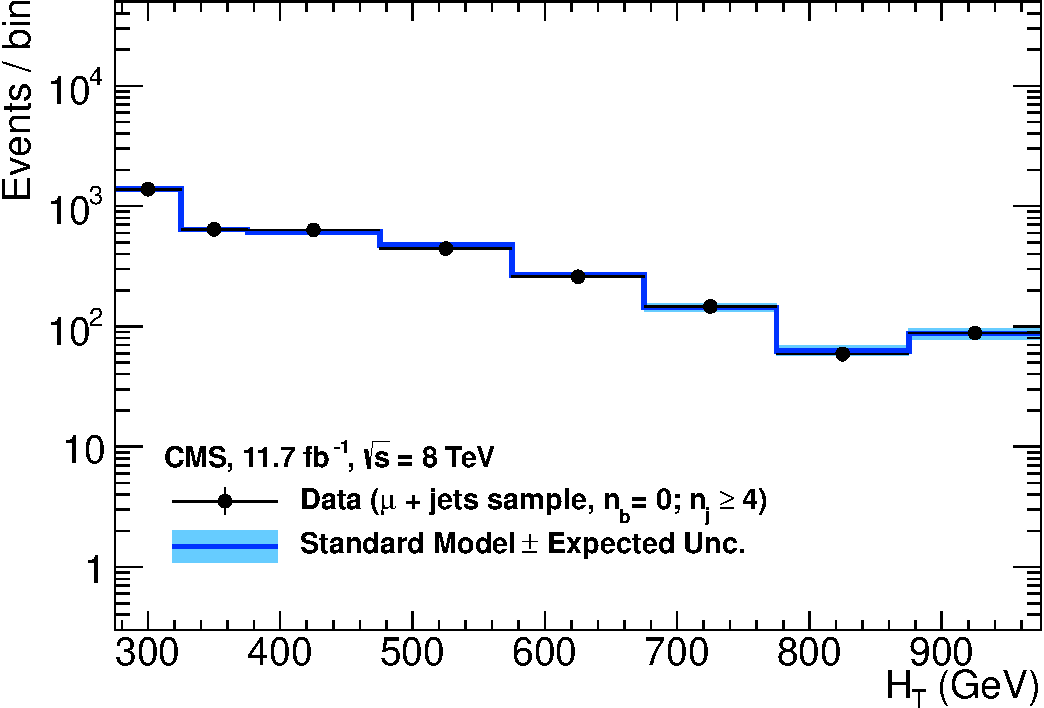
\includegraphics[width = 1.0\linewidth]{plots/muon_0b_ge4j_logy.pdf}
\centering (b)  \mupjets sample, $n_{jet} \geq 4$ and $n_{b}^{reco} = 0$  
\end{minipage} \\
\vspace{0.4cm}
\begin{minipage}[b]{0.48 \linewidth}
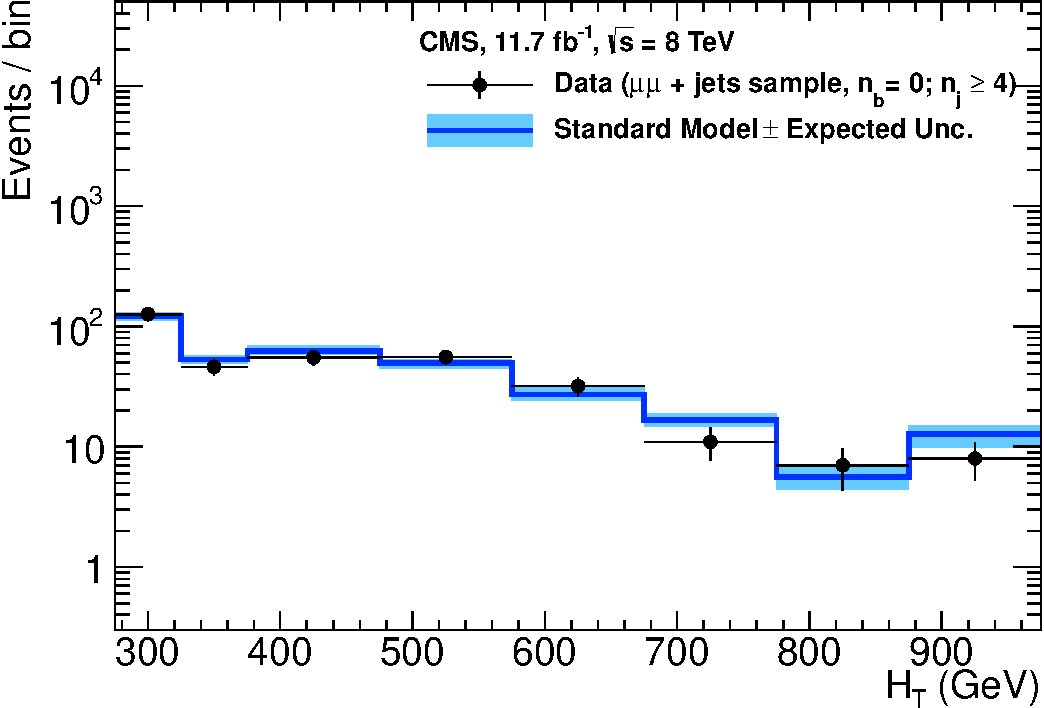
\includegraphics[width = 1.0\linewidth]{plots/mumu_0b_ge4j_logy.pdf}
\centering (c$)$ \dimupjets sample, $n_{jet} \geq 4$ and $n_{b}^{reco} = 0$ 
\end{minipage}
\quad
\begin{minipage}[b]{0.48\linewidth}
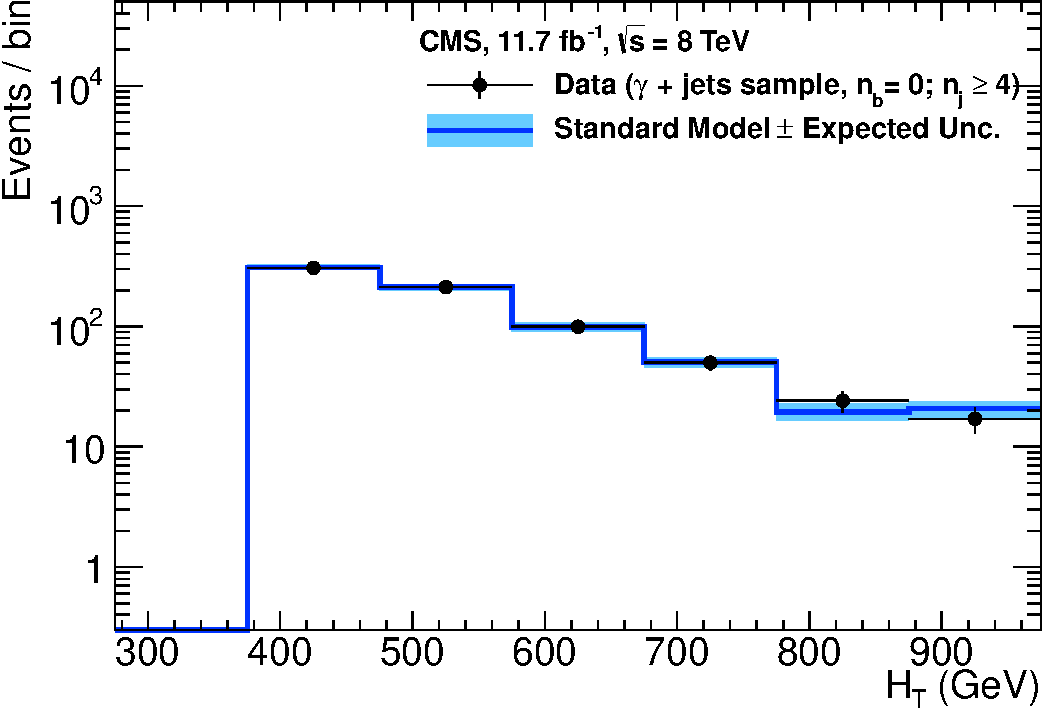
\includegraphics[width = 1.0\linewidth]{plots/photon_0b_ge4j_logy.pdf}
\centering (d)  \gpjets sample, $n_{jet} \geq 4$ and $n_{b}^{reco} = 0$ 
\end{minipage}
\caption[Comparison of the observed yields and \ac{SM} expectations given by the simultaneous fit in bins of \theht for the (a) hadronic, (b) \mupjets, (c$)$ \dimupjets and (d) \gpjets samples when requiring $n_{b}^{reco}$ = 0 and $n_{jet} \geq 4$.]{Comparison of the observed yields and \ac{SM} expectations given by the simultaneous fit in bins of \theht for the (a) hadronic, (b) \mupjets, (c$)$ \dimupjets and (d) \gpjets samples when requiring $n_{b}^{reco}$ = 0 and $n_{jet} \geq 4$. The observed event yields in data (black dots) and the expectations and their uncertainties for all SM processes (blue line with light blue bands) are shown. An example signal expectation (red solid line) for the $D2$ \ac{SMS} signal point from Table \ref{tab:sms_model_table} is superimposed on the \ac{SM} background expectation.}
\label{fig:result0bhigh}
\end{figure}


\begin{figure}[ht]
\footnotesize
\centering
\begin{minipage}[b]{0.48 \linewidth}
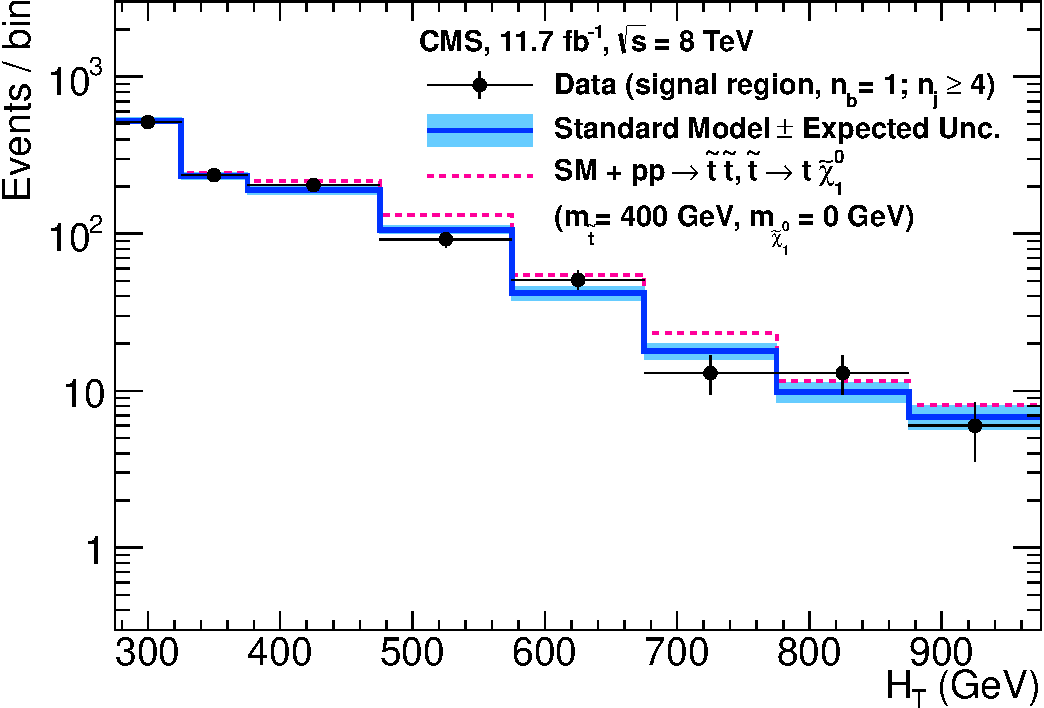
\includegraphics[width = 1.0\linewidth]{plots/hadronic_1b_ge4j_logy.pdf}
\centering (a)  Hadronic sample, $n_{jet} \geq 4$ and $n_{b}^{reco} = 1$ 
\end{minipage}
\quad
\begin{minipage}[b]{0.48\linewidth}
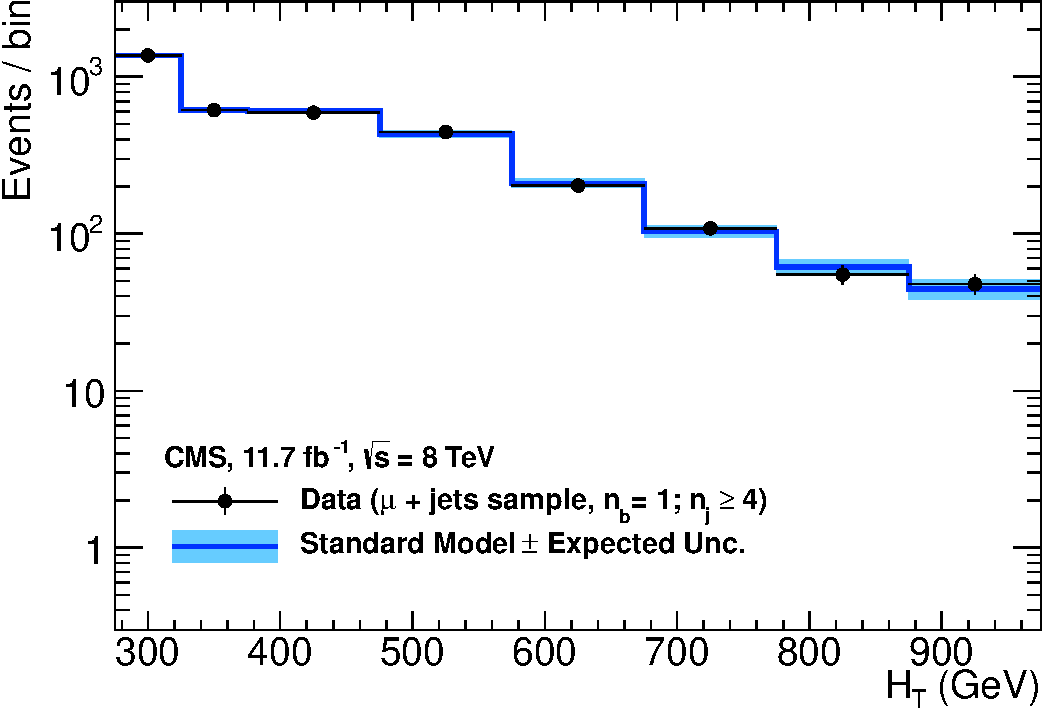
\includegraphics[width = 1.0\linewidth]{plots/muon_1b_ge4j_logy.pdf}
\centering (b)  \mupjets sample, $n_{jet} \geq 4$ and $n_{b}^{reco} = 1$  
\end{minipage} \\
\vspace{0.4cm}
\begin{minipage}[b]{0.48 \linewidth}
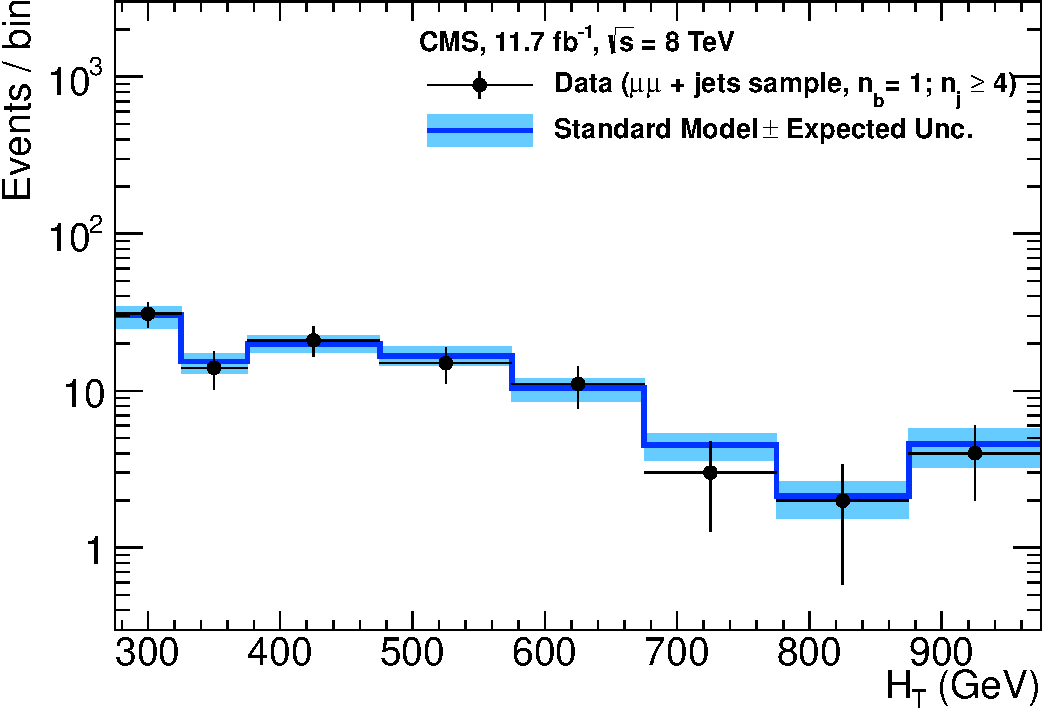
\includegraphics[width = 1.0\linewidth]{plots/mumu_1b_ge4j_logy.pdf}
\centering (c$)$ \dimupjets sample, $n_{jet} \geq 4$ and $n_{b}^{reco} = 1$ 
\end{minipage}
\quad
\begin{minipage}[b]{0.48\linewidth}
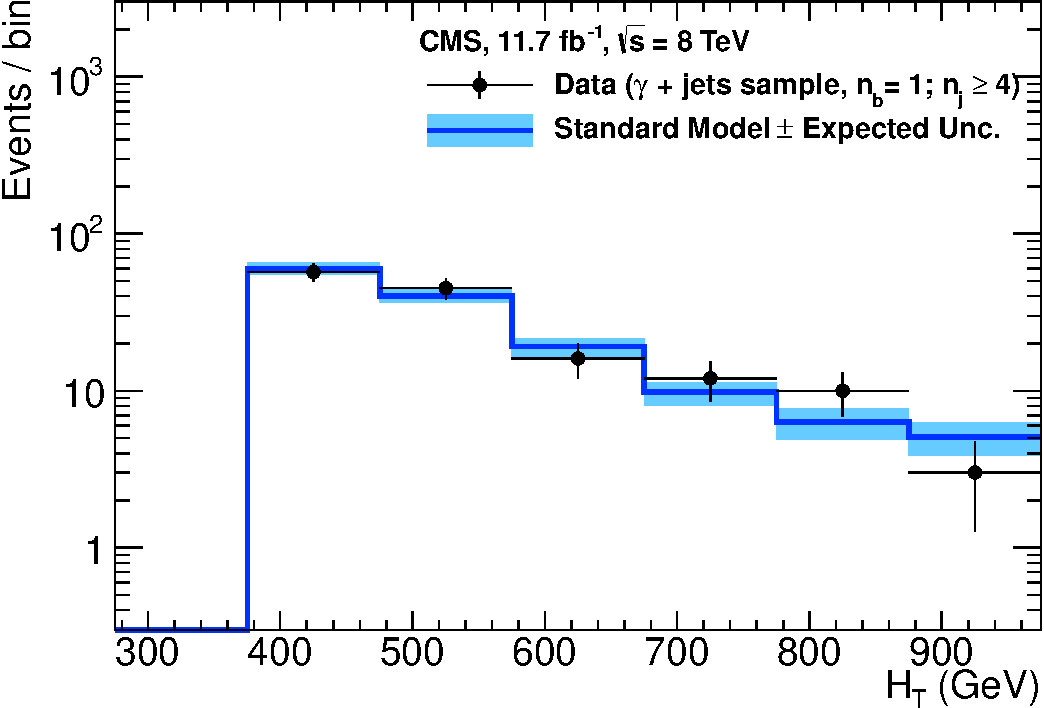
\includegraphics[width = 1.0\linewidth]{plots/photon_1b_ge4j_logy.pdf}
\centering (d)  \gpjets sample, $n_{jet} \geq 4$ and $n_{b}^{reco} = 1$ 
\end{minipage}
\caption[Comparison of the observed yields and \ac{SM} expectations given by the simultaneous fit in bins of \theht for the (a) hadronic, (b) \mupjets, (c$)$ \dimupjets and (d) \gpjets samples when requiring $n_{b}^{reco}$ = 1 and $n_{jet} \geq 4$.]{Comparison of the observed yields and \ac{SM} expectations given by the simultaneous fit in bins of \theht for the (a) hadronic, (b) \mupjets, (c$)$ \dimupjets and (d) \gpjets samples when requiring $n_{b}^{reco}$ = 1 and $n_{jet} \geq 4$. The observed event yields in data (black dots) and the expectations and their uncertainties for all SM processes (blue line with light blue bands) are shown.}
\label{fig:result1bhigh}
\end{figure}

\begin{figure}[ht]
\footnotesize
\centering
\begin{minipage}[b]{0.48 \linewidth}
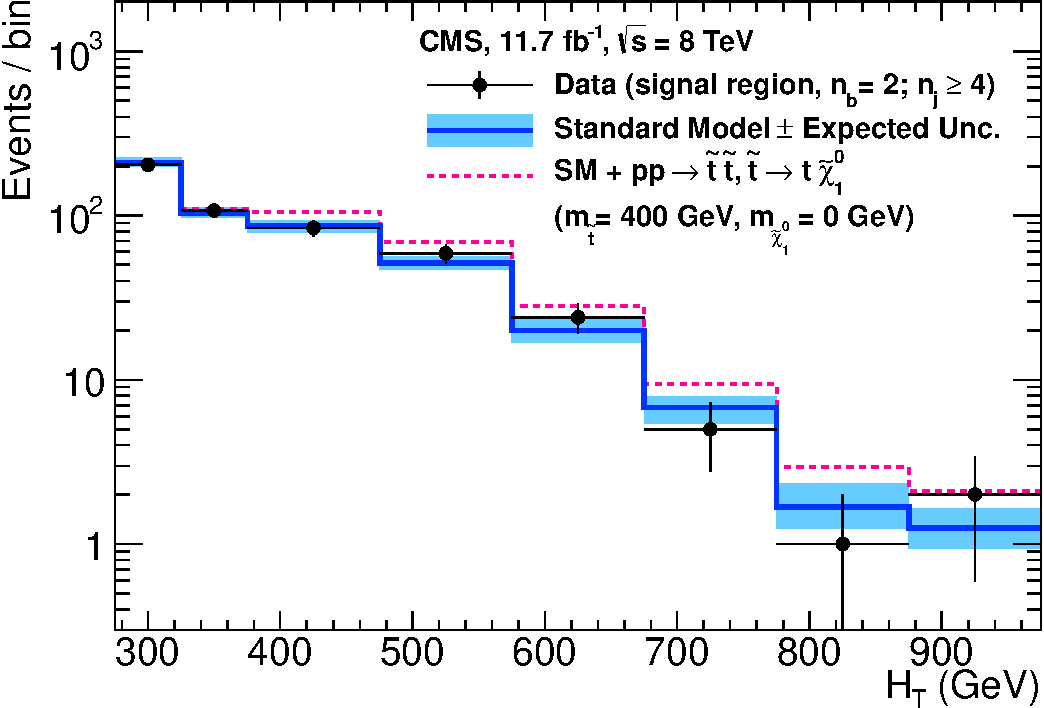
\includegraphics[width = 1.0\linewidth]{plots/hadronic_2b_ge4j_logy.pdf}
\centering (a)  Hadronic sample, $n_{jet} \geq 4$ and $n_{b}^{reco} = 2$ 
\end{minipage}
\quad
\begin{minipage}[b]{0.48\linewidth}
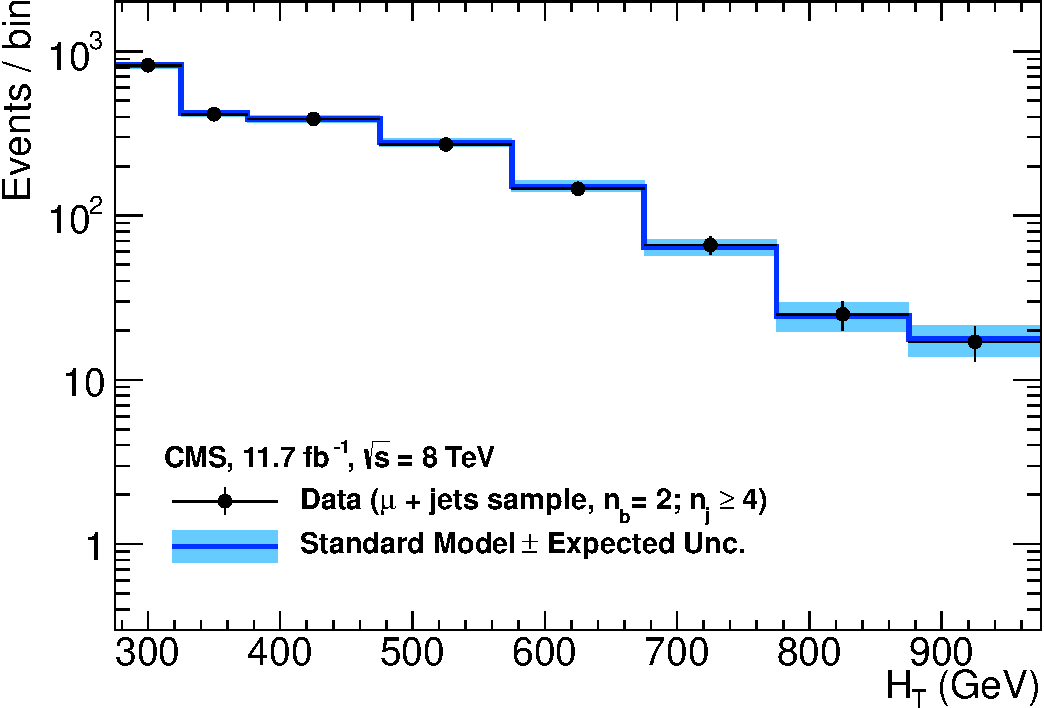
\includegraphics[width = 1.0\linewidth]{plots/muon_2b_ge4j_logy.pdf}
\centering (b)  \mupjets sample, $n_{jet} \geq 4$ and $n_{b}^{reco} = 2$  
\end{minipage} \\
\caption[Comparison of the observed yields and \ac{SM} expectations given by the simultaneous fit in bins of \theht for the (a) hadronic, (b) \mupjets, (c$)$ \dimupjets and (d) \gpjets samples when requiring $n_{b}^{reco}$ = 2 and $n_{jet} \geq 4$.]{Comparison of the observed yields and \ac{SM} expectations given by the simultaneous fit in bins of \theht for the (a) hadronic, (b) \mupjets, (c$)$ \dimupjets and (d) \gpjets samples when requiring $n_{b}^{reco}$ = 2 and $n_{jet} \geq 4$. The observed event yields in data (black dots) and the expectations and their uncertainties for all SM processes (blue line with light blue bands) are shown. An example signal expectation (red solid line) for the $D3$ \ac{SMS} signal point from Table \ref{tab:sms_model_table} is superimposed on the \ac{SM} background expectation.}
\label{fig:result2bhigh}
\end{figure}

\begin{figure}[ht]
\footnotesize
\centering
\begin{minipage}[b]{0.48 \linewidth}
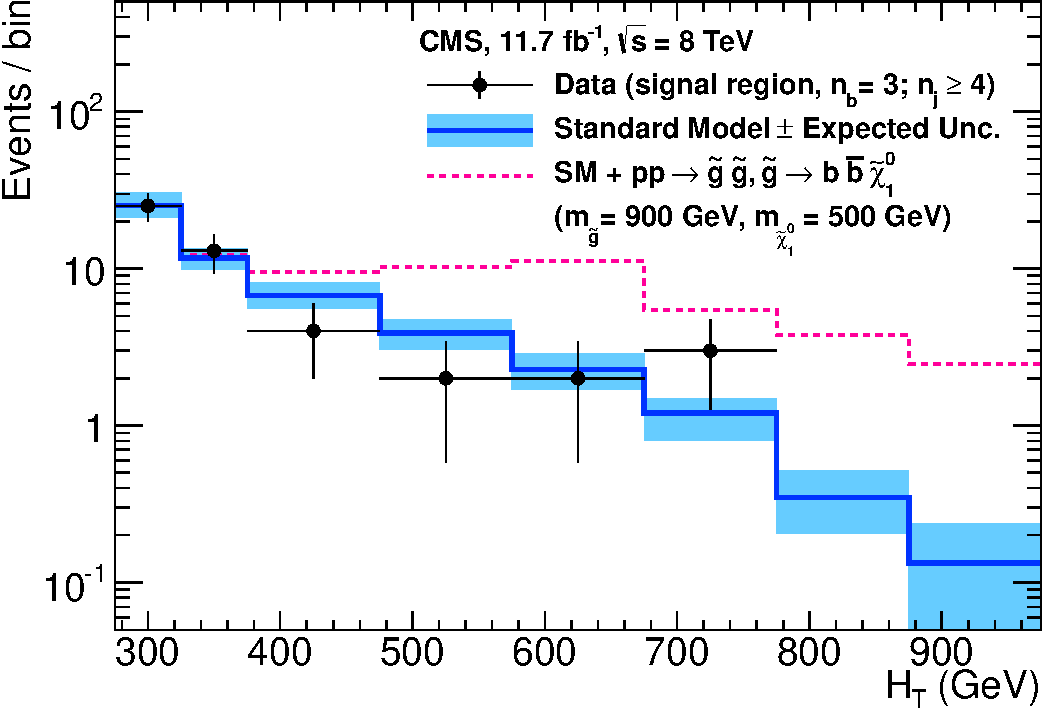
\includegraphics[width = 1.0\linewidth]{plots/hadronic_3b_ge4j_logy.pdf}
\centering (a)  Hadronic sample, $n_{jet} \geq 4$ and $n_{b}^{reco} = 3$ 
\end{minipage}
\quad
\begin{minipage}[b]{0.48\linewidth}
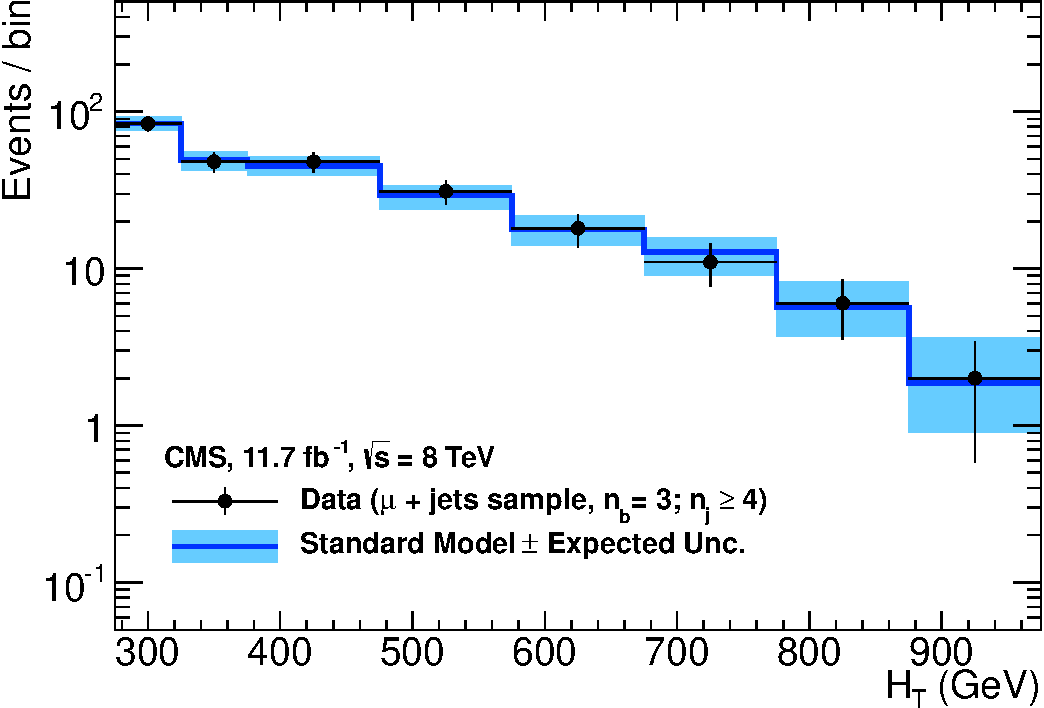
\includegraphics[width = 1.0\linewidth]{plots/muon_3b_ge4j_logy.pdf}
\centering (b)  \mupjets sample, $n_{jet} \geq 4$ and $n_{b}^{reco} = 3$  
\end{minipage} \\
\caption[Comparison of the observed yields and \ac{SM} expectations given by the simultaneous fit in bins of \theht for the (a) hadronic, (b) \mupjets, (c$)$ \dimupjets and (d) \gpjets samples when requiring $n_{b}^{reco}$ = 3 and $n_{jet} \geq 4$.]{Comparison of the observed yields and \ac{SM} expectations given by the simultaneous fit in bins of \theht for the (a) hadronic, (b) \mupjets, (c$)$ \dimupjets and (d) \gpjets samples when requiring $n_{b}^{reco}$ = 3 and $n_{jet} \geq 4$. The observed event yields in data (black dots) and the expectations and their uncertainties for all SM processes (blue line with light blue bands) are shown. An example signal expectation (red solid line) for the $G2$ \ac{SMS} signal point from Table \ref{tab:sms_model_table} is superimposed on the \ac{SM} background expectation.}
\label{fig:result3bhigh}
\end{figure}

\begin{figure}[ht]
\footnotesize
\centering
\begin{minipage}[b]{0.48 \linewidth}
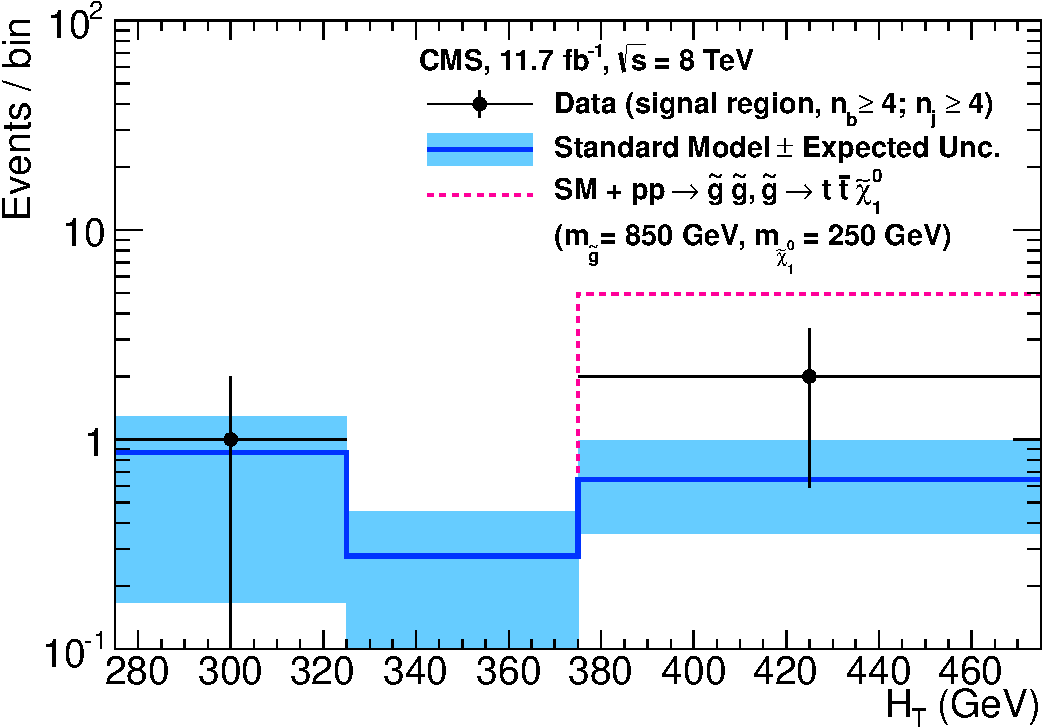
\includegraphics[width = 1.0\linewidth]{plots/hadronic_ge4b_ge4j_logy.pdf}
\centering (a)  Hadronic sample, $n_{jet} \geq 4$ and $n_{b}^{reco} \geq 4$ 
\end{minipage}
\quad
\begin{minipage}[b]{0.48\linewidth}
\includegraphics[width = 1.0\linewidth]{plots/muon_ge4b_ge4j_logy.pdf}
\centering (b)  \mupjets sample, $n_{jet} \geq 4$ and $n_{b}^{reco} \geq 4$  
\end{minipage} \\
\caption[Comparison of the observed yields and \ac{SM} expectations given by the simultaneous fit in bins of \theht for the (a) hadronic, (b) \mupjets, (c$)$ \dimupjets and (d) \gpjets samples when requiring $n_{b}^{reco} \geq$  4 and $n_{jet} \geq 4$.]{Comparison of the observed yields and \ac{SM} expectations given by the simultaneous fit in bins of \theht for the (a) hadronic, (b) \mupjets, (c$)$ \dimupjets and (d) \gpjets samples when requiring $n_{b}^{reco}$ $\geq$ 4 and $n_{jet} \geq 4$. The observed event yields in data (black dots) and the expectations and their uncertainties for all SM processes (blue line with light blue bands) are shown. An example signal expectation (red solid line) for the $G3$ \ac{SMS} signal point from Table \ref{tab:sms_model_table} is superimposed on the \ac{SM} background expectation.}
\label{fig:result4bhigh}
\end{figure}


\section{SUSY}
\label{sec:resultsms}

Limits are set in the parameter space of a set of \ac{SMS} models that characterise both natural \ac{SUSY} third generation squark production, and compressed spectra where the mass splitting between the particle and \ac{LSP} is small, leading to soft final state jets. However as detailed in Section (\ref{subsec:sms}), the individual models are not representative of a real physical \ac{SUSY} model as only one decay process is considered. Instead these models represent a way to test for signs of specific signatures indicating new physics. 

\subsection{The CL$_{\text{s}}$ method}

The CLs method \cite{0954-3899-28-10-313}\cite{Junk1999435}\cite{Read:451614} is used to compute the limits for signal models, with the one-sided profile likelihood ratio as the test statistic \cite{asymptotictest}.

The test statistic is defined as
\begin{equation}
  q(\mu)=\begin{cases}
    -2\text{log}\lambda(\mu) & \text{ when $\mu \geq \hat{\mu}$},\\
      \ \ 0 & \text{otherwise}.
  \end{cases}
\end{equation}

where 

\begin{equation}
\lambda(\mu) = \frac{L(\mu,\theta_{\mu})}{L(\hat{\mu},\hat{\theta})}
\end{equation}

represents the profile likelihood ratio, in which $\mu \equiv f$ from Section (\ref{subsec:signalcontribution}), is the parameter characterising the signal strength.  $\hat{\mu}$ is defined as the maximum likelihood value, $\hat{\theta}$ the set of maximum likelihood values of the nuisance parameters and $\theta_{\mu}$ the set of maximum values of the nuisance parameters for a given value of $\mu$.

When $\mu \equiv f = 1$, the signal model is considered at its nominal production cross section. The distribution of $q_{\mu}$ is built up via the generation of pseudo experiments in order to obtain two distributions for the background (B) and signal plus background (S+B) cases.

The compatibility of a signal model with observations in data is determined by the parameter CL$_{s}$,

\begin{equation}
\text{CL$_{S}$} = \frac{\text{CL$_{S+B}$}}{\text{CL$_{B}$}},
\end{equation}

with CL$_{B}$ and CL$_{S+B}$ defined as one minus the quantiles of the observed value in the data of the two distributions. A model is considered to be excluded at 95\% confidence level when CL$_{s} \leq 0.05$ \cite{2011EPJClimits}.

\subsection{Interpretation in simplified signal models}

Different \njet and \nbreco bins are used in the interpretation of different \ac{SMS} models. The choice of the categories used within each interpretation, are made to maximise the signal to background ratio, increasing sensitivity to that particular type of final state signature. The production and decay modes of the \ac{SMS} models under consideration are summarised in Table \ref{tab:susyresults}, with limit plots of the experimental reach in these models shown in Figure \ref{fig:smslimitplots}.

The models \texttt{T1} and \texttt{T2} are used to characterise the pair production of gluinos and first or second generation squarks, respectively, with parameters for the sparticle mass as well as on the \ac{LSP} mass. The low number of third generation quarks produced from this decay topology makes choosing to interpret within the \nbreco = 0 category beneficial to improving sensitivity to these models.

Conversely the \texttt{T2bb}, \texttt{T1tttt}, and \texttt{T1bbbb} \ac{SMS} models describe various production and decay mechanisms in the context of third-generation squarks. In this situation considering higher \nbreco categories bring significant improvements to the sensitivity to these types of final state signature. 

Finally the choice of jet category is made dependant upon the production mechanism, where gluino induced and direct squark production results in a large or small number of final state jets respectively.

 \begin{table}[h!]
 \footnotesize
\begin{center}
\begin{tabular*}{1.0\textwidth}{@{\extracolsep{\fill}}llcccccc}
\hline
Model & Production/decay & $n_{jet}$ & $n_{b}^{reco}$ & Process & Limit & m$_{\tilde{q}(\tilde{g})}^{\text{best}}$ (\GeV)  & m$_{\text{LSP}}^{\text{best}}$ (\GeV) \\
\hline\hline
\texttt{T1} &  $pp \rightarrow \widetilde{g}\widetilde{g}^{*} \rightarrow q\bar{q}\widetilde{\chi}^{0}_{1}q\bar{q}\widetilde{\chi}^{0}_{1}$ & $\geq 4$ & 0 & \ref{fig:smsprocesses}(a) & \ref{fig:smslimitplots}(a) & $\sim$950 & $\sim$450 \\
\texttt{T2}  & $ pp \rightarrow \widetilde{q}\widetilde{q}^{*} \rightarrow q\widetilde{\chi}^{0}_{1}\bar{q}\widetilde{\chi}^{0}_{1}$ & $\leq 3$ & 0 & \ref{fig:smsprocesses}(b) & \ref{fig:smslimitplots}(b) & $\sim$775 &  $\sim$325 \\
\texttt{T2bb} & $ pp \rightarrow \widetilde{b}\widetilde{b}^{*} \rightarrow b\widetilde{\chi}^{0}_{1}\bar{b}\widetilde{\chi}^{0}_{1}$ & $\leq 3$ & 1,2 & \ref{fig:smsprocesses}(c$)$ & \ref{fig:smslimitplots}(c$)$ & $\sim$600 & $\sim$200\\
\texttt{T1tttt} & $ pp \rightarrow \widetilde{g}\widetilde{g}^{*} \rightarrow t\bar{t}\widetilde{\chi}^{0}_{1}t\bar{t}\widetilde{\chi}^{0}_{1}$ & $\geq 4$ & 2,3,$\geq4$ & \ref{fig:smsprocesses}(d) & \ref{fig:smslimitplots}(d) & $\sim$975 & $\sim$325 \\
\texttt{T1bbbb} & $ pp \rightarrow \widetilde{g}\widetilde{g}^{*} \rightarrow b\bar{b}\widetilde{\chi}^{0}_{1}b\bar{b}\widetilde{\chi}^{0}_{1}$ & $\geq 4$ & 2,3,$\geq4$ & \ref{fig:smsprocesses}(e) & \ref{fig:smslimitplots}(e) & $\sim$1125 & $\sim$650 \\
\hline
\end{tabular*}
\end{center}
\caption[A table representing the \ac{SMS} models interpreted within the analysis.]{A table representing the \ac{SMS} models interpreted within the analysis. The model name and production and decay chain is specified in the first two columns. Each \ac{SMS} model is interpreted in specific $n_{jet}$ and $n_{b}^{reco}$ categories which are detailed in the third and fourth columns. The last two columns indicate the search sensitivity for each model, representing the largest $m_{\widetilde{q}/\widetilde{g}}$ mass beyond which no limit can be set for this particular decay topology. The quoted values are conservatively determined from the observed exclusion based on the theoretical production cross section minus 1$\sigma$ uncertainty.}\label{tab:susyresults}
\end{table}


Experimental uncertainties on the \ac{SM} background predictions (10 $-$ 30\%, described in Section (\ref{subsec:determinesystematics})), the luminosity measurement (4.4\%), and the total acceptance times efficiency of the selection for the considered signal model (12 $-$18\%, from Section (\ref{sec:smsmodels})) are included in the calculation of the limit. 

Signal efficiency in the kinematic region defined by 0 $< m_{\widetilde{g}(\widetilde{q})} <$ 175 \GeV or $m_{\widetilde{g}(\widetilde{q})} <$ 300 \GeV is strongly affected by the presence of \acf{ISR}. This region in which direct (i.e. non-\ac{ISR} induced) production is kinematically forbidden due to the \theht $>$ 275 \GeV requirement, therefore a large percentage of signal acceptance is due to the effect of \ac{ISR} jets. Given the large associated uncertainties, no interpretation is provided for this kinematic region.

The estimates on mass limits shown in Table  \ref{tab:susyresults}, are determined conservatively from the observed exclusion based on the theoretical production cross section, minus 1$\sigma$ uncertainty. The most stringent mass limits on pair-produced sparticles are obtained at low \ac{LSP} masses and larger squark and gluino masses due to the high \pt jets and consequently high \theht of such signal topologies. The limits are seen to weaken for compressed spectra points closer to the diagonal, where the signal populates the lower \theht bins in which more background resides. For all of the considered models, there is an \ac{LSP} mass beyond which no limit can be set, which can be observed from the figures referenced in the table. 

Two small upwards fluctuations are observed within the data, and are seen at high \theht within the \nbreco = 0 category and at mid-\theht in the \nbreco = 1, 2 categories, see Table \ref{tab:fitsdata}. As each of these fluctuations occur within at least one of the analysis categories that each \ac{SMS} model interpretation is made, the observed exclusions within all \ac{SMS} models are generally found to be weaker than the expected limits in the region of 1-2 standard deviations. In isolation these fluctuations are not significant and additional data would be necessary to make any further conclusions.

Despite these fluctuations, the range of parameter space that can be excluded has been extended with respect to analysis based upon the $\sqrt{s} = 7$ \TeV dataset \cite{Chatrchyan:2012wa}, by up to 225 and 150 \GeV for m$_{\tilde{q}(\tilde{g})}^{\text{best}}$ and m$_{LSP}^{\text{best}}$ respectively. The parameter space for light third generation squarks, the main tenet of natural \ac{SUSY} models, is increasingly squeezed for larger mass splitting, with exclusions in the region of 1 \TeV in these topologies. 



\begin{figure}[ht]
\footnotesize
\centering
\begin{minipage}[b]{0.48 \linewidth}
\includegraphics[width = 1.0\linewidth]{plots/t1susydecay.pdf}
\centering \caption*{(a) $\widetilde{g}\widetilde{g}^{*} \rightarrow q\bar{q}\widetilde{\chi}^{0}_{1}q\bar{q}\widetilde{\chi}^{0}_{1}$ (\texttt{T1})}\label{f`ig:t1}
\end{minipage}
\quad
\begin{minipage}[b]{0.48\linewidth}
\includegraphics[width = 1.0\linewidth]{plots/t2susydecay.pdf}
\centering \caption*{(b) $\widetilde{q}\widetilde{q}^{*} \rightarrow q\widetilde{\chi}^{0}_{1}\bar{q}\widetilde{\chi}^{0}_{1}$ (\texttt{T2})} \label{fig:t2}
\end{minipage} \\
\vspace{0.4cm}
\begin{minipage}[b]{0.48 \linewidth}
\includegraphics[width = 1.0\linewidth]{plots/t2bbsusydecay.pdf}
\centering \caption*{(c$)$ $\widetilde{b}\widetilde{b}^{*} \rightarrow b\widetilde{\chi}^{0}_{1}\bar{b}\widetilde{\chi}^{0}_{1}$ (\texttt{T2bb})} \label{fig:t2bb}
\end{minipage}
\quad
\begin{minipage}[b]{0.48\linewidth}
\includegraphics[width = 1.0\linewidth]{plots/t1ttttsusydecay.pdf}
\centering \caption*{(d) $\widetilde{g}\widetilde{g}^{*} \rightarrow t\bar{t}\widetilde{\chi}^{0}_{1}t\bar{t}\widetilde{\chi}^{0}_{1}$ (\texttt{T1tttt})} \label{fig:t2tttt}
\end{minipage}
\quad
\begin{minipage}[b]{0.48\linewidth}
\centering
\includegraphics[width = 1.0\linewidth]{plots/t1bbbbsusydecay.pdf}
\centering \caption*{(e) $\widetilde{g}\widetilde{g}^{*} \rightarrow b\bar{b}\widetilde{\chi}^{0}_{1}b\bar{b}\widetilde{\chi}^{0}_{1}$ (\texttt{T1bbbb})} \label{fig:t1bbbb}
\end{minipage}
\caption[Production and decay modes for the various \ac{SMS} models interpreted within the analysis.]{Production and decay modes for the various \ac{SMS} models interpreted within the analysis.}
\label{fig:smsprocesses}
\end{figure}

\begin{figure}[ht]
\footnotesize
\centering
\begin{minipage}[b]{0.48 \linewidth}
\includegraphics[width = 1.0\linewidth]{plots/t1.pdf}
\centering \caption*{(a) $\widetilde{g}\widetilde{g}^{*} \rightarrow q\bar{q}\widetilde{\chi}^{0}_{1}q\bar{q}\widetilde{\chi}^{0}_{1}$ (\texttt{T1})}\label{fig:t1}
\end{minipage}
\quad
\begin{minipage}[b]{0.48\linewidth}
\includegraphics[width = 1.0\linewidth]{plots/t2.pdf}
\centering \caption*{(b) $\widetilde{q}\widetilde{q}^{*} \rightarrow q\widetilde{\chi}^{0}_{1}\bar{q}\widetilde{\chi}^{0}_{1}$ (\texttt{T2})} \label{fig:t2}
\end{minipage} \\
\vspace{0.4cm}
\begin{minipage}[b]{0.48 \linewidth}
\includegraphics[width = 1.0\linewidth]{plots/t2bb.pdf}
\centering \caption*{(c$)$ $\widetilde{b}\widetilde{b}^{*} \rightarrow b\widetilde{\chi}^{0}_{1}\bar{b}\widetilde{\chi}^{0}_{1}$ (\texttt{T2bb})} \label{fig:t2bb}
\end{minipage}
\quad
\begin{minipage}[b]{0.48\linewidth}
\includegraphics[width = 1.0\linewidth]{plots/t1tttt.pdf}
\centering \caption*{(d) $\widetilde{g}\widetilde{g}^{*} \rightarrow t\bar{t}\widetilde{\chi}^{0}_{1}t\bar{t}\widetilde{\chi}^{0}_{1}$ (\texttt{T1tttt})} \label{fig:t2tttt}
\end{minipage}
\quad
\begin{minipage}[b]{0.48\linewidth}
\centering
\includegraphics[width = 1.0\linewidth]{plots/t1bbbb.pdf}
\centering \caption*{(e) $\widetilde{g}\widetilde{g}^{*} \rightarrow b\bar{b}\widetilde{\chi}^{0}_{1}b\bar{b}\widetilde{\chi}^{0}_{1}$ (\texttt{T1bbbb})} \label{fig:t1bbbb}
\end{minipage}
\caption[Upper limit of cross section at 95\% CL as a function of $m_{\widetilde{q}/\widetilde{g}}$ and $m_{LSP}$ for various \ac{SMS} models.]{Upper limit of cross section at 95\% CL as a function of $m_{\widetilde{q}/\widetilde{g}}$ and $m_{LSP}$ for various \ac{SMS} models. The solid thick black line indicates the observed exclusion region assuming \ac{NLO} and \ac{NLL}  SUSY production cross section. The analysis selection efficiency is measured for each interpreted model, with the signal yield per point given by $\epsilon \times \sigma$ 
. The thin black lines represent the observed excluded region when varying the cross section by its theoretical uncertainty. The dashed purple lines indicate the median (thick line) �1$\sigma$ (thin lines) expected exclusion regions.}
\label{fig:smslimitplots}
\end{figure}




  %% To ignore a specific chapter while working on another,
  %% making the build faster, comment it out like this:
\end{mainmatter}

%% Produce the appendices
%\begin{appendices}
%  %% The "\appendix" call has already been made in the declaration
%% of the "appendices" environment (see thesis.tex).

\chapter{Miscellaneous}
\label{app:noise}
\section{Noise Filters}

For Calo jets the following criteria were applied:

\begin{table}[H]
\footnotesize
\begin{center}
\begin{tabulary}{0.80\textwidth}{LL}
\cline{1-2}
\multicolumn{2}{l}{Loose CaloJet Id} \\
Variable & Definition \\ 
\hline\hline
f$_{HPD} < 0.98$ \qquad\qquad\qquad\qquad\qquad\qquad & Fraction of jet energy contributed from ``hottest'' \ac{HPD}, which rejects \ac{HCAL} noise.  \\
f$_{EM} > 0.01$ & Noise from the \ac{HCAL} is further suppressed by requiring a minimal electromagnetic component to the jet f$_{EM}$. \\
N$^{90}_{hits} \geq$ 2 & Jets that have $>$ 90\% of its energy from a single chanel are rejected, to serve as a safety net that catches jets arising from undiagnosed noisy channels.\\
\hline
\end{tabulary}
\end{center}
\caption[Criteria for a reconstructed jet to pass the loose calorimeter jet id.]{Criteria for a reconstructed jet to pass the loose calorimeter jet id.}
\label{tabapp:calojetid}
\end{table}


For PF jets the following criteria were applied:
  
\begin{table}[H]
\footnotesize
\begin{center}
\begin{tabulary}{0.80\textwidth}{p{3.5cm}L}
\cline{1-2}
\multicolumn{2}{l}{Loose PF jet Id} \\
Variable & Definition \\ 
\hline\hline
nfhJet $<$ 0.99 & Fraction of jet composed of neutral hadrons. \ac{HCAL} noise tends to populate high values of neutral 
hadron fraction.\\
nemfJet $<$ 0.99 & Fraction of jet composed of neutral electromagnetic energy. \ac{ECAL} noise tends to populate high values of 
neutral EM fraction. \\
nmultiJet $>$ 1 & Number of constituents that jet is composed from. \\
chfJet $>$ 0 & Fraction of jet composed of charged hadrons. \\
cmultiJet $>$ 0 & Number of charged particles that compose jet. \\
cemfJet $<$ 0.99 & Fraction of jet composed of charged electromagnetic energy. \\
\hline
\end{tabulary}
\end{center}
\caption[Criteria for a reconstructed jet to pass the loose PF jet id.]{Criteria for a reconstructed jet to pass the loose PF jet id.}
\label{apptab:pfjetid}
\end{table}  
  
   
The following noise filters are applied, to remove events with spurious, non-physical jets or missing transverse energy.

\begin{table}[H]
\footnotesize
\begin{center}
\begin{tabulary}{0.80\textwidth}{p{4cm}L}
\cline{1-2}
\multicolumn{2}{l}{Noise Filters} \\
Variable & Definition \\ 
\hline\hline
 CSC tight beam halo filter \qquad\qquad\qquad\qquad\qquad & As proton beams circle the \ac{lhc}, proton interactions with the residual gas particles or the beam collimators can occur, producing showers of secondary particles which can interact with the \ac{CMS} detector. \\
 HBHE noise filter with isolated noise rejection & Anomalous noise in the \ac{HCAL} not due to electronics noise, but rather due to instrumentation issues associated with the \ac{HPD}'s and \acf{RBXs}. \\
 HCAL laser filter & The \ac{HCAL} uses laser pulses for monitoring the detector response. Some laser pulses have accidentally been fired in the physics orbit, and ended up polluting events recorded for physics analysis. \\
 ECAL dead cell trigger primitive (TP) filter & \ac{EB} and \ac{EE} have single noisy crystals which are masked in reconstruction. Use the \acf{TP} information to assess how much energy was lost in masked cells. \\
 Bad EE Supercrystal filter & Two supercrystals in \ac{EE} are found to occasionally produce high amplitude anomalous pulses in several channels at once, causing a large \met spike. \\
 ECAL Laser correction filter & A laser calibration multiplicative factor is applied to correct for transparency loss in each crystal during irradiation. A small number of crystals receive unphysically large values of this correction and become very energetic, resulting in \met. \\
\cline{1-2}
\end{tabulary}
\end{center}
\caption[Noise filters that are applied to remove spurious and non-physical \met signatures within the \ac{CMS} detector.]{Noise filters that are applied to remove spurious and non-physical \met signatures within the \ac{CMS} detector.}
\label{apptab:noiseid}
\end{table}  

\section{Primary Vertices}

\label{app:primaryvertices}

The pileup per event is defined by the number of 'good' reconstructed primary vertices in the event, with each vertex satisfying the following requirements

\begin{table}[H]
\footnotesize
\begin{center}
\begin{tabulary}{0.80\textwidth}{p{3cm}L}
\cline{1-2}
\multicolumn{2}{l}{Good primary vertex requirement} \\
Variable & Definition \\ 
\hline\hline
$N_{dof} > 4$ \qquad\qquad\qquad & The number of degree of freedom, from the vertex fit to compute the best estimate of the vertex parameters. \\
$\vert \Delta z_{vtx} \vert < 24$cm &  The distance, $\vert\Delta z_{vex}\vert$, to the position of the closest \ac{HLT} primary vertex. \\ 
 $\rho < 2$cm & The perpendicular distance of track position to the beam spot. \\
\cline{1-2}
\end{tabulary}
\end{center}
\caption[Criteria for a vertex in an event to be classified as a 'good' reconstructed primary vertex.]{Criteria for a vertex in an event to be classified as a 'good' reconstructed primary vertex.}
\label{tabapp:primaryvertices}
\end{table}

\chapter{L1 Jets}

\section{Jet matching efficiencies}
\label{app:jetmatching}

The single jet turn-on curves are derived from events independent of wether the leading jet in an event is matched to a Level 1 jet using $\Delta R$ matching detailed in Section  (\ref{subsec:l1jettrigeff}) or not.  These turn-ons are produced from events which are not triggered on jet quantities and therefore it is not guaranteed that the lead jet of an event will be seeded by a Level 1 jet. Figure \ref{fig:leadjetmatcheff} shows the particular matching efficiency of a lead jet to a L1 jet.

\begin{figure}[htp]
\centering
\resizebox{.7\linewidth}{0.5\height}{\includegraphics{plots/leadjet_matchingeff.pdf}}
\caption[Leading jet matching efficiency as a function of the offline CaloJet $\et$.]{Leading jet matching efficiency as a function of the offline CaloJet $\et$, measured in an isolated muon triggered dataset in the 2012B and 2012C run periods.}
  \label{fig:leadjetmatcheff}
\end{figure}

It can be seen that the turn on is sharper during the 2012B run
period. The seed threshold requirement of a 5 \GeV jet seed in run 2012C results
in more events in which even the lead offline jet does not have an associated L1 jet. For larger jet $\et$
thresholds, typical of thresholds used in physics analyses, 100$\%$ efficiency is observed.

The matching efficiencies have a $\mu$ values of 6.62 GeV and 19.51 GeV for Run 2012B and 2012C respectively and is shown in Table~\ref{tab:matcheff}. 

\begin{table}
\begin{center}
\begin{tabular*}{0.5\textwidth}{c|cc}
\cline{1-3}
\multicolumn{1}{c}{Run Period} & $\mu$ & $\sigma$ \\ \hline\hline
2012B & 6.62 $\pm$ 0.01 & 0.79 $\pm$ 0.03  \\ 
2012C & 19.51 $\pm$ 0.03 & 7.14 $\pm$ 0.02 \\ 
\end{tabular*}
\caption[Results of a cumulative EMG function fit to the turn-on
curves for the matching efficiency of the leading jet in an event to
a Level-1 jet in run 2012C and 2012B data.]{Results of a cumulative EMG function fit to the turn-on
curves for the matching efficiency of the leading jet in an event to
a Level-1 jet in run 2012C and 2012B data, measured in an isolated
muon triggered sample. The turn-on point, $\mu$, and resolution, $\sigma$, are measured with respect to offline Calo Jet $\et$.} \label{tab:matcheff}
\end{center}
\end{table}

\section{Leading Jet Energy Resolution}
\label{app:jetpuresolution}

\begin{figure}[htp]

    \centering
    \subfloat[]{  \includegraphics[width=0.95\textwidth]{plots/ptresolution_low.pdf}  }\,
    %\caption{}
\end{figure}

\begin{figure}
    %\ContinuedFloat
    \centering
    \subfloat[]{\includegraphics[width=0.95\textwidth]{plots/ptresolution_medium.pdf}}\,
    \subfloat[]{\includegraphics[width=0.95\textwidth]{plots/ptresolution_high.pdf}}\,

      \caption[ Resolution plots of the leading offline \Calo $\et$ measured as a function of  $\frac{(\text{L1 E}_{T} -  \text{Offline E}_{T})}{\text{Offline E}_{T}}$ for  low (a), medium (b) and high (c) pile-up conditions.] { Resolution plots of the leading offline jet \Calo $\et$ measured as a function of  $\frac{(\text{L1 E}_{T} -  \text{Offline E}_{T})}{\text{Offline E}_{T}}$ for  low (a), medium (b) and high (c) pile-up conditions. }
\end{figure}

\begin{figure}[htpb]

    \centering
    \subfloat[]{  \includegraphics[width=0.95\textwidth]{plots/ptresolution_low.pdf}  }\,
    \subfloat[]{\includegraphics[width=0.95\textwidth]{plots/ptresolution_medium.pdf}}\,

\end{figure}

\begin{figure}
   % \ContinuedFloat
    \centering
    \subfloat[]{\includegraphics[width=0.95\textwidth]{plots/ptresolution_high.pdf}}\,

      \caption[ Resolution plots of the leading off-line PF $\et$ measured as a function of  $\frac{(\text{L1 E}_{T} -  \text{Offline E}_{T})}{\text{Offline E}_{T}}$ for  low (a), medium (b) and high (c) pile-up conditions.] { Resolution plots of the leading offline jet \PF $\et$ measured as a function of  $\frac{(\text{L1 E}_{T} -  \text{Offline E}_{T})}{\text{Offline E}_{T}}$ for  low (a), medium (b) and high (c) pile-up conditions. }
  
\end{figure}


\newpage
\section{Resolution for Energy Sum Quantities}
\label{app:jetenergysums}

The following plots show the resolution parameters for the four energy sum quantities as a function of the quantity (q) itself. In this case, The mean and RMS of the individual $\frac{(\text{L1 q} -  \text{Offline q})}{\text{Offline q}}$ distributions, in bins of the quantity q is displayed. 

\begin{figure}[h!]
  \vspace{20pt}
        \centering
        \includegraphics[width=1.0\textwidth]{plots/res_CaloSumET_summary.pdf}
        \caption[$\sum$ $\et$~resolution parameters in bins of Calo $\sum E_{T}$  measured for the defined low, medium and high pile up conditions.]{$\sum$ $\et$~resolution parameters in bins of Calo $\sum E_{T}$  measured for the defined low, medium and high pile up conditions. The plots show the mean $\mu$ (left), resolution $\sigma$ (RMS) of the $\frac{\Delta q}{q}$ distributions.}
        \label{fig:caloetresultspu}
\end{figure}
\begin{figure}[h!]
  \vspace{20pt}
  \centering
        \includegraphics[width=1.0\textwidth]{plots/res_pfSumET_summary.pdf}
        \caption[$\sum$ $\et$~resolution parameters in bins of PF $\sum E_{T}$  measured for the defined low, medium and high pile up conditions. ]{$\sum$ $\et$~resolution parameters in bins of PF $\sum E_{T}$  measured for the defined low, medium and high pile up conditions. The plots show the mean $\mu$ (left), resolution $\sigma$ (RMS) of the $\frac{\Delta q}{q}$ distributions.}
        \label{fig:pfetresultspu}
\end{figure}

\begin{figure}[h!]
  \vspace{20pt}
        \centering
        \includegraphics[width=1.0\textwidth]{plots/res_CaloMET_summary.pdf}
        \caption[$\met$~resolution parameters in bins of Calo $\met$~ measured for the defined low, medium and high pile up conditions.]{$\met$~resolution parameters in bins of Calo $\met$~ measured for the defined low, medium and high pile up conditions. The plots show the mean $\mu$ (left), resolution $\sigma$ (RMS) of the $\frac{\Delta q}{q}$  distributions.}
        \label{fig:calometresultspu}
\end{figure}
\begin{figure}[h!]
  \vspace{20pt}
        \centering
        \includegraphics[width=1.0\textwidth]{plots/res_pfMET_summary.pdf}
        \caption[$\met$~resolution parameters in bins of PF $\met$~ measured for the defined low, medium and high pile up conditions.]{$\met$~resolution parameters in bins of PF $\met$~ measured for the defined low, medium and high pile up conditions. The plots show the mean $\mu$ (left), resolution $\sigma$ (RMS) of the $\frac{\Delta q}{q}$  distributions.}
        \label{fig:pfmetresultspu}
\end{figure}


\begin{figure}[h!]
  \vspace{20pt}
        \centering
        \includegraphics[width=1.0\textwidth]{plots/res_CaloHT_summary.pdf}
        \caption[$\theht$~resolution parameters in bins of Calo $\theht$~measured for the defined low, medium and high pile up conditions. ]{$\theht$~resolution parameters in bins of Calo $\theht$~measured for the defined low, medium and high pile up conditions. The plots show the mean $\mu$ (left), resolution $\sigma$ (RMS) of the $\frac{\Delta q}{q}$ distributions.}
        \label{fig:calohtresultspu}
\end{figure}
\begin{figure}[h!]
  \vspace{20pt}
        \centering
        \includegraphics[width=1.0\textwidth]{plots/res_pfHT_summary.pdf}
        \caption[$\theht$~resolution parameters in bins of PF $\theht$~measured for the defined low, medium and high pile up conditions.]{$\theht$~resolution parameters in bins of PF $\theht$~measured for the defined low, medium and high pile up conditions. The plots show the mean $\mu$ (left), resolution $\sigma$ (RMS) of the $\frac{\Delta q}{q}$ distributions.}
        \label{fig:pfhtresultspu}
\end{figure}

\begin{figure}[h!]
  \vspace{20pt}
        \centering
        \includegraphics[width=1.0\textwidth]{plots/res_CaloMHT_summary.pdf}
        \caption[$\mht$~resolution parameters in bins of $\mht$~measured for the defined low, medium and high pile up conditions.]{$\mht$~resolution parameters in bins of $\mht$~measured for the defined low, medium and high pile up conditions. The plots show the mean $\mu$ (left), resolution $\sigma$ (RMS) of the $\frac{\Delta q}{q}$ distributions.}
        \label{fig:calomhtresultspu}
\end{figure}
\begin{figure}[h!]
  \vspace{20pt}
        \centering
        \includegraphics[width=1.0\textwidth]{plots/res_pfMHT_summary.pdf}
        \caption[$\mht$~resolution parameters in bins of PF $\mht$~measured for the defined low, medium and high pile up conditions.]{$\mht$~resolution parameters in bins of PF $\mht$~measured for the defined low, medium and high pile up conditions. The plots show the mean $\mu$ (left), resolution $\sigma$ (RMS) of the $\frac{\Delta q}{q}$ distributions.}
        \label{fig:pfmhtresultspu}
\end{figure}

\chapter{Additional material on background estimation methods}
\label{app:backgroundestimation}
\section{Determination of $k_{QCD}$}
\label{app:kqcd}


\begin{minipage}{\linewidth}
\centering
\includegraphics[width = 4.9in]{plots/qcd_sideband_fits.pdf}
\captionof{figure}[$R_{\alphat}$(\theht) and exponential fits for each of the data sideband regions. Fit is conducted between the \theht region 275 $<$ \theht $<$ 575.]{$R_{\alphat}$(\theht) and exponential fits for each of the data sideband regions. Fit is conducted between the \theht region 275 $<$ \theht $<$ 575.}
\label{fig:qcd_sideband_fits}
\end{minipage}


\section{Effect of varying background cross sections on closure tests }
\label{app:xsecvariation}

Closure tests with cross section variations of +20\% and -20\% applied to W + jets and \ttbar processes respectively.

\begin{figure}[ht]
\centering
\begin{minipage}[b]{0.48 \linewidth}
\includegraphics[width = 1.0\linewidth]{plots/syst-le3j_nominal.pdf}
\centering
(a)  
\end{minipage}
\quad
\begin{minipage}[b]{0.48\linewidth}
\includegraphics[width = 1.0\linewidth]{plots/syst-le3j_varied.pdf}
\centering
(b) 
\end{minipage}
\caption[Sets of closure tests overlaid on top of the systematic uncertainty used for each of the five \theht regions.]{Sets of closure tests (open symbols) overlaid on top of the systematic uncertainty used for each of the five \theht regions (shaded bands) and for the two different jet multiplicity bins:(a) $2 \leq n_{jet} \leq 3$ and (b) $n_{jet} \geq 4$.}
\label{fig:xsecvariedle3j}
\end{figure}


\begin{figure}[ht]
\centering
\begin{minipage}[b]{0.48 \linewidth}
\includegraphics[width = 1.0\linewidth]{plots/syst-ge4j_nominal.pdf}
\centering
(a)  
\end{minipage}
\quad
\begin{minipage}[b]{0.48\linewidth}
\includegraphics[width = 1.0\linewidth]{plots/syst-ge4j_varied.pdf}
\centering
(b) 
\end{minipage}
\caption[Sets of closure tests overlaid on top of the systematic uncertainty used for each of the five \theht regions.]{Sets of closure tests (open symbols) overlaid on top of the systematic uncertainty used for each of the five \theht regions (shaded bands) and for the two different jet multiplicity bins:(a) $2 \leq n_{jet} \leq 3$ and (b) $n_{jet} \geq 4$.}
\label{fig:xsecvariedge4j}
\end{figure}

 \begin{table}[h!]
\begin{center}
\begin{tabular*}{0.95\textwidth}{@{\extracolsep{\fill}}cl|cccc}
\cline{1-6}
&&\multicolumn{4}{l}{\theht (\GeV)} \\
\cline{1-6}
\cline{1-6}
\end{tabular*}
\end{center}
\caption[ ]{}\label{tab:xsecvaried}
\end{table}

\chapter{Additional Material  For B-tag Template Method}
\label{app:templatematerial}
\section{Templates Fits in Simulation}
\label{app:templatemc}


\begin{figure}[ht]
\centering
\begin{minipage}[b]{0.55 \linewidth}
\includegraphics[width = 1.0\linewidth]{plots/template_mc_loose_njet3.pdf}
\centering (a) Loose working point $n_{jet}$ = 3 
\end{minipage}
\quad
\begin{minipage}[b]{0.55\linewidth}
\includegraphics[width = 1.0\linewidth]{plots/template_mc_medium_njet3.pdf}
\centering (b) Medium working point $n_{jet}$ = 3 
\end{minipage}
\quad
\begin{minipage}[b]{0.55\linewidth}
\centering
\includegraphics[width = 1.0\linewidth]{plots/template_mc_high_njet3.pdf}
\centering (c) Tight working point $n_{jet} =$ 3 
\end{minipage}
\caption[The results of fitting the Z = 0 and Z = 2 templates to the $n_{b}^{reco}$ = 0, 1, 2 bins taken directly from simulation in the region \theht $>$ 375 \GeV, for the $n_{jet} = 3$ category.]{The results of fitting the Z = 0 and Z = 2 templates to the $n_{b}^{reco}$ = 0, 1, 2 bins taken directly from simulation in the region \theht $>$ 375 \GeV, for the $n_{jet} = 3$ category. The red template represents Z = 0, while the blue template represents Z = 2. Grey bands represent the statistical uncertainty of the fit.The $\chi^{2}$ parameter displayed represents the goodness of fit to the low$ n_{b}^{reco}$ (0-2) control region.}
\label{app:template_closure_njet3}
\end{figure}

\begin{figure}[ht]
\centering
\begin{minipage}[b]{0.55 \linewidth}
\includegraphics[width = 1.0\linewidth]{plots/template_mc_loose_njet4.pdf}
\centering (a) Loose working point $n_{jet}$ = 4 
\end{minipage}
\quad
\begin{minipage}[b]{0.55\linewidth}
\includegraphics[width = 1.0\linewidth]{plots/template_mc_medium_njet4.pdf}
\centering (b) Medium working point $n_{jet}$ = 4 
\end{minipage}
\quad
\begin{minipage}[b]{0.55\linewidth}
\centering
\includegraphics[width = 1.0\linewidth]{plots/template_mc_high_njet4.pdf}
\centering (c) Tight working point $n_{jet} =$ 4 
\end{minipage}
\caption[The results of fitting the Z = 0 and Z = 2 templates to the $n_{b}^{reco}$ = 0, 1, 2 bins taken directly from simulation in the region \theht $>$ 375 \GeV, for the $n_{jet} = 4$ category.]{The results of fitting the Z = 0 and Z = 2 templates to the $n_{b}^{reco}$ = 0, 1, 2 bins taken directly from simulation in the region \theht $>$ 375 \GeV,  for the $n_{jet} = 4$ category. The red template represents Z = 0, while the blue template represents Z = 2. Grey bands represent the statistical uncertainty of the fit.The $\chi^{2}$ parameter displayed represents the goodness of fit to the low$ n_{b}^{reco}$ (0-2) control region.}
\label{fig:template_closure_high}
\end{figure}

\FloatBarrier

\section{Pull Distributions for Template Fits}
\label{app:templatepulldistributions}

\section{Templates Fits in Data}
\label{app:templatedata}

Template fits for the loose \ac{CSV} working point :

\begin{figure}[ht]
\centering
\begin{minipage}[b]{0.48 \linewidth}
\includegraphics[width = 1.0\linewidth]{plots/template_data_medium_njet5_lowht.pdf}
\centering (a) $n_{jet} \geq$  5 , 275 $<$ \theht $<$ 325
\end{minipage}
\quad
\begin{minipage}[b]{0.48\linewidth}
\includegraphics[width = 1.0\linewidth]{plots/template_data_medium_njet5_midht.pdf}
\centering (b) $n_{jet} \geq$ = 5 , 325 $<$ \theht $<$ 375 
\end{minipage}
\quad
\begin{minipage}[b]{0.48\linewidth}
\centering
\includegraphics[width = 1.0\linewidth]{plots/template_data_medium_njet5_highht.pdf}
\centering (c) $n_{jet} \geq$ 5 , \theht $\geq$ 375 
\end{minipage}
\caption[The results of fitting the Z = 0 and Z = 2 templates to the $n_{b}^{reco}$ = 0, 1, 2 bins taken directly from data, for the $n_{jet} \geq 5$ category and loose \ac{CSV} working point.]{The results of fitting the Z = 0 and Z = 2 templates to the $n_{b}^{reco}$ = 0, 1, 2 bins taken from data, for the $n_{jet} \geq 5$ category and loose \ac{CSV} working point. The red template represents Z = 0, while the blue template represents Z = 2. The $\chi^{2}$ parameter displayed represents the goodness of fit to the low$ n_{b}^{reco}$ (0-2) control region.}
\label{app:template_data_loose_njet5}
\end{figure}
\FloatBarrier

Template fits for the tight \ac{CSV} working point :

\begin{figure}[ht]
\centering
\begin{minipage}[b]{0.48 \linewidth}
\includegraphics[width = 1.0\linewidth]{plots/template_data_medium_njet5_lowht.pdf}
\centering (a) $n_{jet} \geq$  5 , 275 $<$ \theht $<$ 325
\end{minipage}
\quad
\begin{minipage}[b]{0.48\linewidth}
\includegraphics[width = 1.0\linewidth]{plots/template_data_medium_njet5_midht.pdf}
\centering (b) $n_{jet} \geq$ = 5 , 325 $<$ \theht $<$ 375 
\end{minipage}
\quad
\begin{minipage}[b]{0.48\linewidth}
\centering
\includegraphics[width = 1.0\linewidth]{plots/template_data_medium_njet5_highht.pdf}
\centering (c) $n_{jet} \geq$ 5 , \theht $\geq$ 375 
\end{minipage}
\caption[The results of fitting the Z = 0 and Z = 2 templates to the $n_{b}^{reco}$ = 0, 1, 2 bins taken directly from data, for the $n_{jet} \geq 5$ category and tight \ac{CSV} working point.]{The results of fitting the Z = 0 and Z = 2 templates to the $n_{b}^{reco}$ = 0, 1, 2 bins taken from data, for the $n_{jet} \geq 5$ category and tight \ac{CSV} working point. The red template represents Z = 0, while the blue template represents Z = 2. The $\chi^{2}$ parameter displayed represents the goodness of fit to the low$ n_{b}^{reco}$ (0-2) control region.}
\label{app:template_data_tight_njet5}
\end{figure}

%\end{appendices}

%% Produce the un-numbered back matter (e.g. colophon,
%% bibliography, tables of figures etc., index...)
\begin{backmatter}
  %\begin{colophon}
%  This thesis was made in \LaTeXe{} using the ``hepthesis'' class~\cite{hepthesis}.
%\end{colophon}

%% You're recommended to use the eprint-aware biblio styles which
%% can be obtained from e.g. www.arxiv.org. The file mythesis.bib
%% is derived from the source using the SPIRES Bibtex service.
%\bibliographystyle{h-physrev}



\bibliographystyle{ieeetr}
\bibliography{mythesis}


\section*{Acronyms}

\begin{acronym}[AAAAAAA]
\acro{ALICE}[ALICE]{A Large Ion Collider Experiment}
\acro {ATLAS} [ATLAS] {A Toroidal LHC ApparatuS}
\acro{APD}[APD]{Avalanche Photo-Diodes}
\acro{BSM}[BSM]{Beyond Standard Model}
\acro {CERN} [CERN] {European Organization for Nuclear Research}
\acro {CMS} [CMS] {Compact Muon Solenoid}
\acro {CMSSM} [CMSSM] {Compressed Minimal SuperSymmetric Model}
\acro {CSC} [CSC] {Cathode Stripe Chamber}
\acro {CSV} [CSV] {Combined Secondary Vertex}
\acro {CSVM} [CSVM] {Combined Secondary Vertex Medium Working Point}
\acro {DT} [DT] {Drift Tube}
\acro {ECAL} [ECAL] {Electromagnetic CALorimeter}
\acro {EB} [EB] {Electromagnetic CALorimeter Barrel}
\acro {EE} [EE] {Electromagnetic CALorimeter Endcap}
\acro {ES} [ES] {Electromagnetic CALorimeter pre-Shower}
\acro {EMG} [EMG] {Exponentially Modified Gaussian}
\acro {EPJC} [EPJC] {European Physical Journal C}
\acro {EWK} [EWK] {Electroweak Sector}
\acro {GCT} [GCT] {Global Calorimeter Trigger}
\acro {GMT} [GMT] {Global MuonTrigger}
\acro {GT} [GT] {Global Trigger}
\acro {HB} [HB] {Hadron Barrel}
\acro {HCAL} [HCAL] {Hadronic CALorimeter}
\acro {HE} [HE] {Hadron Endcaps}
\acro {HF} [HF] {Hadron Forward}
\acro {HLT}[HLT] {Higher Level Trigger}
\acro {HO} [HO] {Hadron Outer}
\acro {HPD} [HPD] {Hybrid Photo Diode}
\acro {ISR} [ISR] {Initial State Radiation}
\acro {LUT} [LUT] {Look Up Table}
\acro {L1} [L1] {Level 1 Trigger}
\acro{lhc}[LHC]{Large Hadron Collider}
\acro{LHCb}[LHCb]{Large Hadron Collider Beauty}
\acro{LSP}[LSP]{Lightest Supersymmetric Partner}
\acro{NLL}[NLL]{Next to Leading Logorithmic Order}
\acro{NLO}[NLO]{Next to Leading Order}
\acro{NNLO}[NNLO]{Next to Next Leading Order}
\acro{POGs}[POGs]{Physics Object Groups}
\acro{PS}[PS]{Proton Synchrotron}
\acro{QED}[QED]{Quantum Electro-Dynamics}
\acro{QCD}[QCD]{Quantum Chromo-Dynamics}
\acro{QFT}[QFT]{Quantum Field Theory}
\acro {RBXs} [RBXs] {Readout Boxes}
\acro {RPC} [RPC] {Resistive Plate Chamber}
\acro {RCT} [RCT] {Regional Calorimeter Trigger}
\acro {RMT} [RMT] {Regional Muon Trigger}
\acro{SUSY}[SUSY]{SUperSYmmetry}
\acro{SM}[SM]{Standard Model}
\acro{SMS}[SMS]{Simplified Model Spectra}
\acro{SPS}[SPS]{Super Proton Synchrotron}
\acro{TF}[TF]{Transfer Factor}
\acro{TP}[TP]{Trigger Primative}
\acro{VEV}[VEV]{Vacuum Expectation Value}
\acro{VPT}[VPT]{Vacuum Photo-Triodes}
\acro{WIMP}[WIMP]{Weakly Interacting Massive Particle}

\end{acronym}


%% I prefer to put these tables here rather than making the
%% front matter seemingly interminable. No-one cares, anyway!


%%\listoffigures
%%\listoftables
%% If you have time and interest to generate a (decent) index,
%% then you've clearly spent more time on the write-up than the 
%% research ;-)
%\printindex

\end{backmatter}

%% Close
\end{document}
